\documentclass[11pt,DIV=10,final]{scrreprt} %11pt legt die generelle Schriftgrösse fest, DIV die Seitenaufteilung (Seitenränder): lieber viele Seiten als zu kleine Seitenränder!
%ändert man "final" zu "draft'', werden speicheraufwändige Elemente nicht eingebunden: Genau das richtige für die Plagiatsprüfung
%*************** Paket-Einbindungen: ******************
\usepackage[utf8]{inputenc} %damit man auch Umlaute eingeben kann
\usepackage[bitstream-charter]{mathdesign} % Charter als Standardschriftart
\usepackage[scaled=.82]{DejaVuSansMono} % DejaVuSansMono als Code-Schriftart
\usepackage[T1]{fontenc} %damit Umlaute bei einer pdf-Suche auch erkannt werden
\usepackage{amsfonts,amsmath} %Verwendung von Mathematik-Schriftarten
\usepackage{graphicx} %für Grafiken der Formate jpg, png, pdf
\usepackage{float} % um Abbildung wirklich genau dort zu platzieren
\usepackage{url} %für die gute Darstellung von Internet-Links
\usepackage{hyperref} %für die gute Darstellung von Internet-Links
% \usepackage[ngerman]{babel} %deutsches Sprachpaket
\usepackage[ngerman,english]{babel} %deutsches Sprachpaket
\usepackage[round]{natbib} %für vereinfachte:wen/Querverweise
\usepackage{listings} % für Quelltext mit Syntax-Highlighting
\usepackage{listings-rust}
\usepackage{hyperref}
\usepackage{tikz} %für tikz-Grafiken
\usepackage{paracol}
\usepackage{subfigure}
\usepackage{quoting}
\usepackage{capt-of}

\usetikzlibrary{graphs} %für Graphen (also auch Neuronale Netze) in tikz

%************** Zusätzliche Einstellungen und eigene Befehle:  **********
\setkomafont{sectioning}{\rmfamily\bfseries\boldmath} % verwende für die Titel die selbe Schriftart wie für Fliesstext

\tikzset{>=stealth} % schönere Pfeilspitzen in TikZ-Grafiken
\lstset{
	backgroundcolor=\color[HTML]{E8F2F2},
    breaklines=true,
	basicstyle=\small\ttfamily,
	keywordstyle=\color{blue},
	commentstyle=\color{brown},
	numbers=left,
	%numberstyle=\tiny,
	%frame=leftline,
	%xleftmargin=.04\textwidth,
	inputencoding=utf8,
	extendedchars=true,
	literate={ä}{{\"a}}1 {à}{{\`a}}1 {ö}{{\"o}}1 {ü}{{\"u}}1 {è}{{\`e}}1 {é}{{\'e}}1}

\lstnewenvironment{rustcode}[1][] % für abgesetzten rust code
{\lstset{
	language=Rust,
	backgroundcolor=\color[HTML]{E8F2F2},
    breaklines=ture,
	basicstyle=\small\ttfamily,
	keywordstyle=\color{blue},
	commentstyle=\color{brown},
	numbers=left,
	%numberstyle=\tiny,
	%frame=leftline,
	%xleftmargin=.04\textwidth,
	inputencoding=utf8,
	extendedchars=true,
	literate={ä}{{\"a}}1 {à}{{\`a}}1 {ö}{{\"o}}1 {ü}{{\"u}}1 {è}{{\`e}}1 {é}{{\'e}}1,
	#1}}{}

\lstnewenvironment{wslcode}[1][] % für abgesetzten rust code
{\lstset{
	backgroundcolor=\color[HTML]{E8F2F2},
	basicstyle=\small\ttfamily,
    breaklines=ture,
	keywordstyle=\color{blue},
	commentstyle=\color{brown},
	numbers=left,
	%numberstyle=\tiny,
	%frame=leftline,
	%xleftmargin=.04\textwidth,
	inputencoding=utf8,
	extendedchars=true,
	literate={ä}{{\"a}}1 {à}{{\`a}}1 {ö}{{\"o}}1 {ü}{{\"u}}1 {è}{{\`e}}1 {é}{{\'e}}1,
	#1}}{}

\lstnewenvironment{bashcode}[1][] % für abgesetzten rust code
{\lstset{
	language=bash,
	backgroundcolor=\color[HTML]{E8F2F2},
    breaklines=ture,
	basicstyle=\small\ttfamily,
	keywordstyle=\color{blue},
	commentstyle=\color{brown},
	%numberstyle=\tiny,
	%frame=leftline,
	%xleftmargin=.04\textwidth,
	inputencoding=utf8,
	extendedchars=true,
	literate={ä}{{\"a}}1 {à}{{\`a}}1 {ö}{{\"o}}1 {ü}{{\"u}}1 {è}{{\`e}}1 {é}{{\'e}}1,
	#1}}{}
	

\providecommand{\rustinline}{\lstinline[language=Rust,basicstyle=\ttfamily,keywordstyle=\color{blue},commentstyle=\color{brown}, literate={ä}{{\"a}}1 {à}{{\`a}}1 {ö}{{\"o}}1 {ü}{{\"u}}1 {è}{{\`e}}1 {é}{{\'e}}1]} % für Inline-C++ Code


\providecommand{\bashinline}{\lstinline[language=bash,basicstyle=\ttfamily,keywordstyle=\color{blue},commentstyle=\color{brown}, literate={ä}{{\"a}}1 {à}{{\`a}}1 {ö}{{\"o}}1 {ü}{{\"u}}1 {è}{{\`e}}1 {é}{{\'e}}1]} % für Inline-C++ Code

% \setcitestyle{numbers,open={[},close={]}}
% \newcommand{\mi}{\mathrm{i}} %% roman "i"
\newcommand{\mi}{{\text{i}}}
\newcommand{\compconj}[1]{%
  \overline{#1}%
}

\newcommand{\deriv}[2]{%
  \frac{d#1}{d#2}
}

\renewcommand{\lstlistingname}{Code Snippet} % Listing->Code

\begin{document}

\begin{titlepage}
\mbox{}\vspace{0.1\textheight}
\begin{center}
\textbf{\Huge Approximating the Time Independent Schrödinger Equation}\\[3ex]
Gian Laager\\
\today
\vspace{0.05\textheight}
\begin{center}
	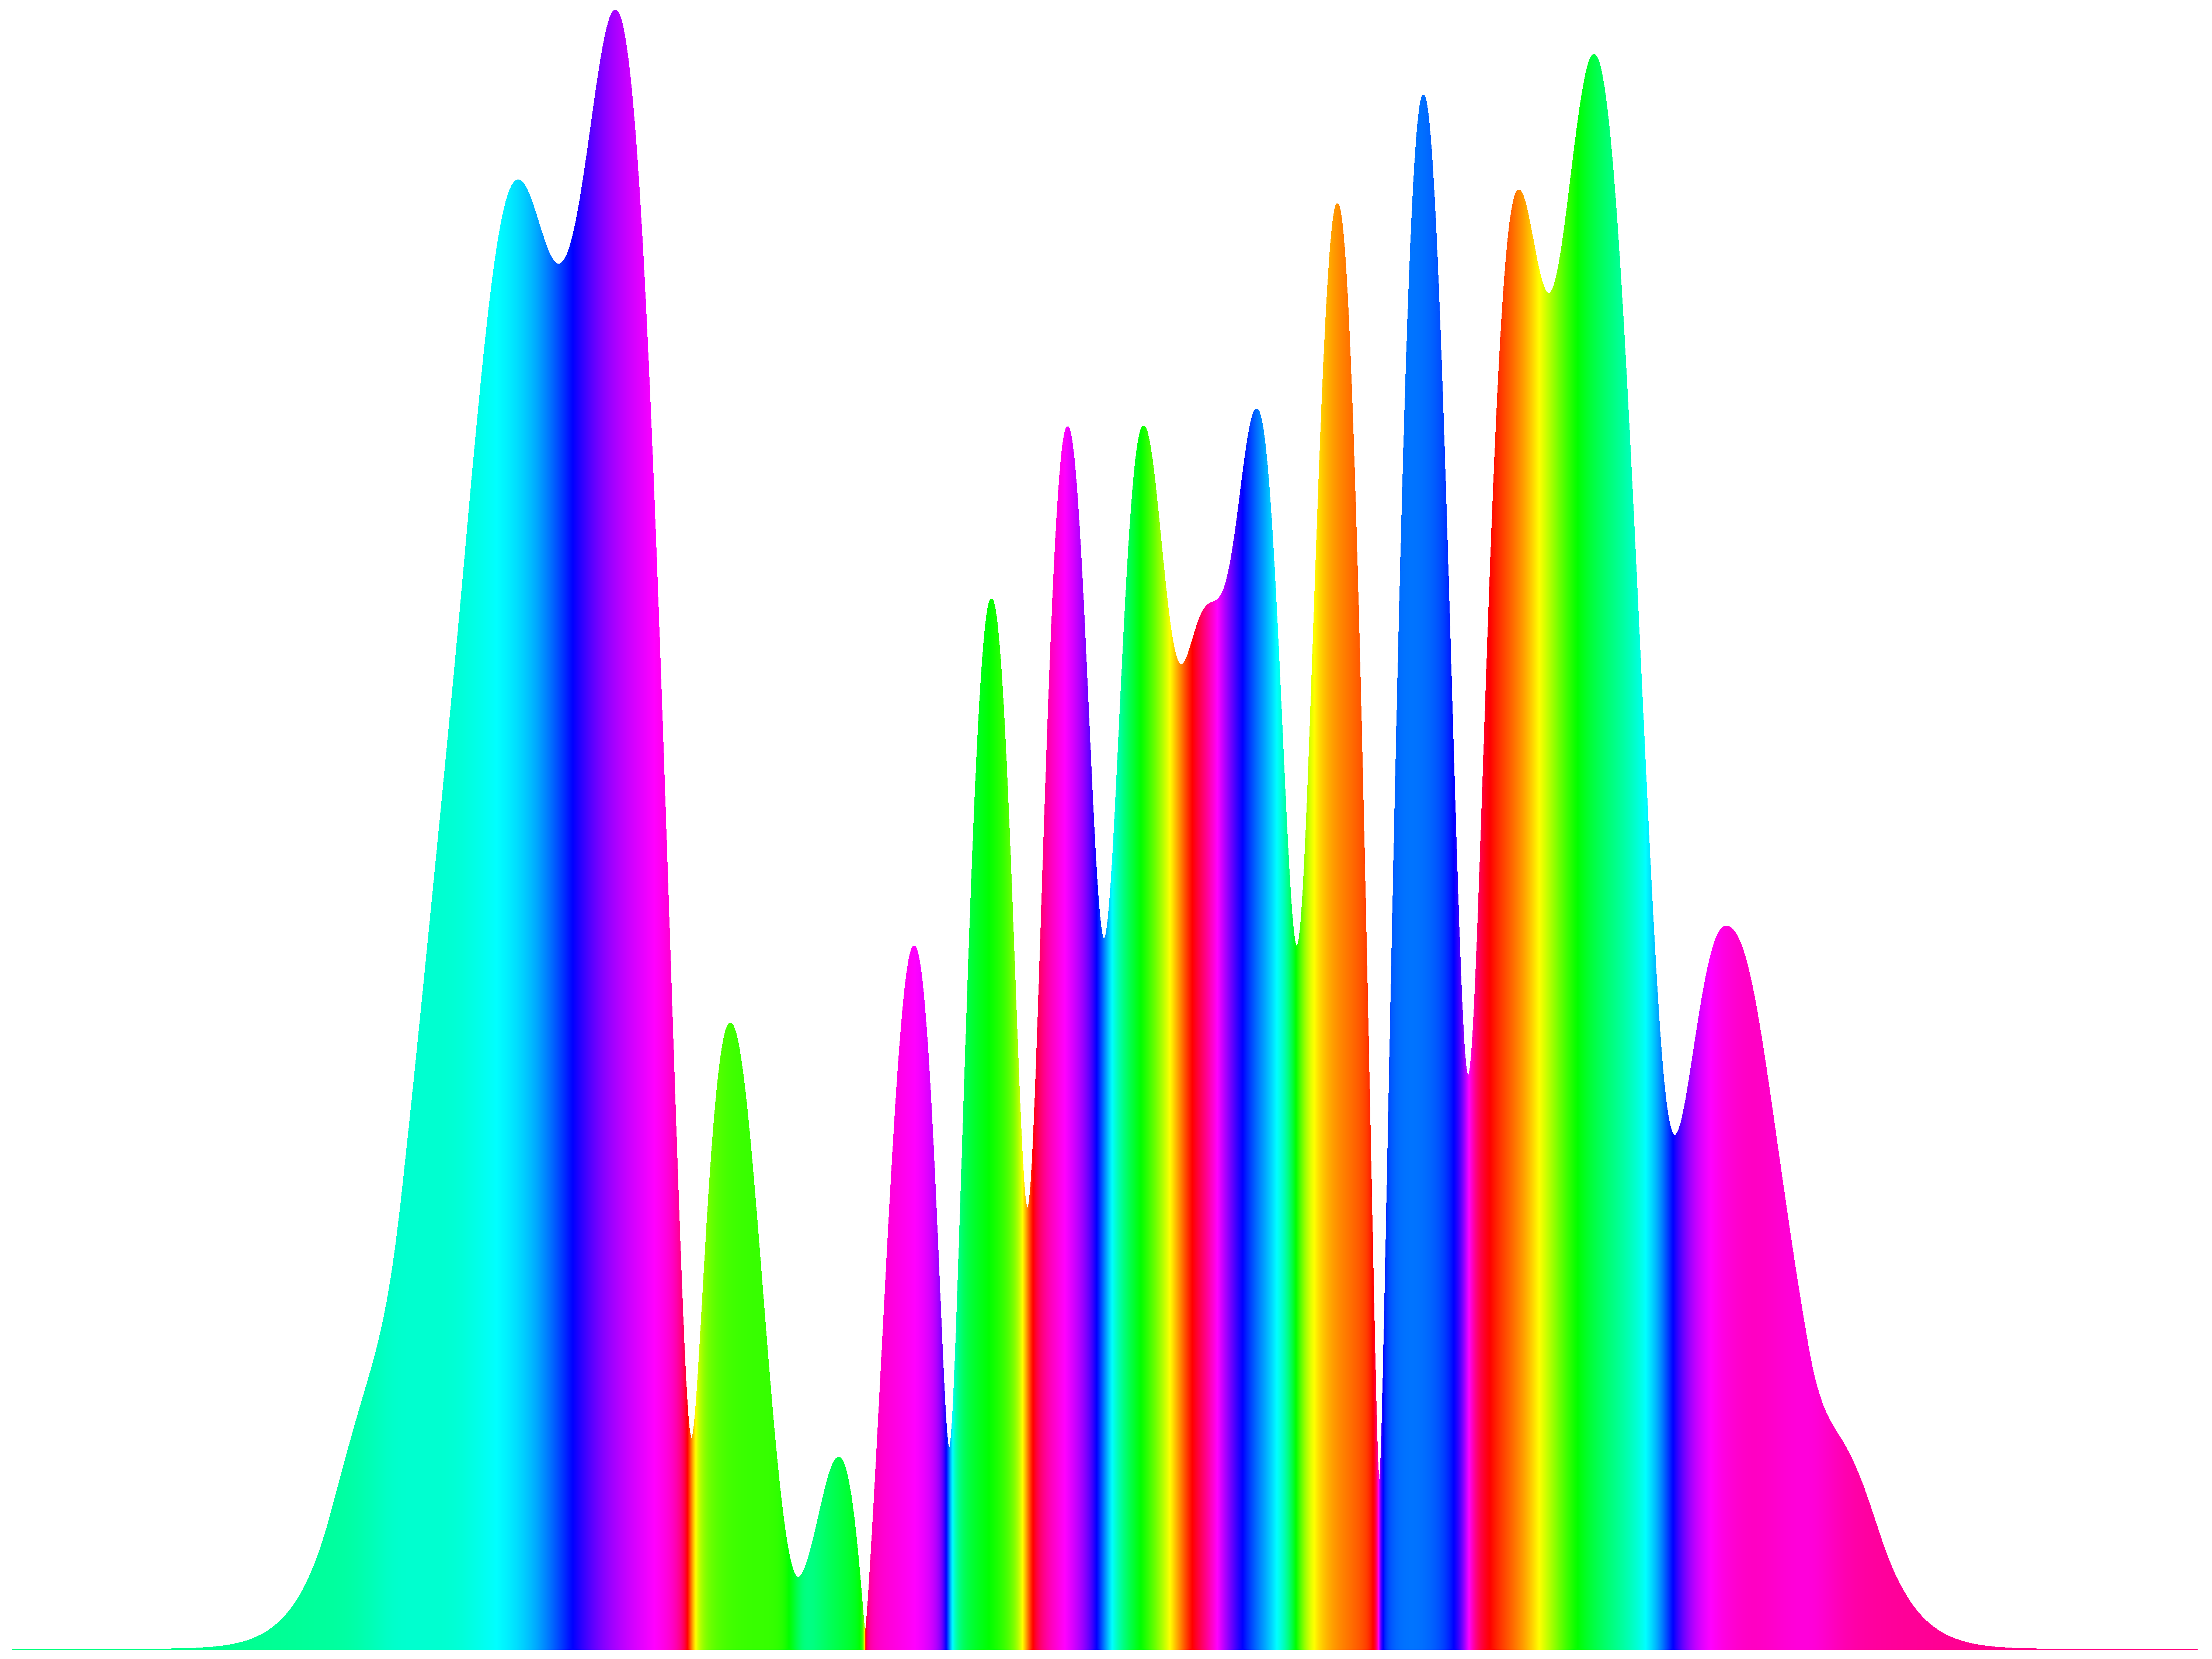
\includegraphics[width=0.9\textwidth]{plots/super-square-9-12-15-title.pdf}
\end{center}
\vspace{0.05\textheight}
Matura thesis\\
Kantonsschule Glarus\\[3ex]
Supervisor: Linus Romer\\
Referent: Dr. Elena Borisova
\end{center}
\end{titlepage}

\pagenumbering{roman}   % i, ii, iii, iv, ...

\tableofcontents

\pagebreak[4]

\chapter*{Vorwort}
\addcontentsline{toc}{chapter}{\protect\numberline{}Vorwort}
Ich habe mich entschieden, eine kleine Zusammenfassung auf deutsch zu schreiben, damit zumindest jeder die Grundlagen meiner Arbeit versteht.

Zu Beginn des 20. Jahrhunderts gab es einen Umschwung in der Physik. Die Quantenmechanik wurde entdeckt. Diese neue Theorie kann nicht mehr präzise Voraussagen machen, wie es zuvor der Fall war.
Man kann nur noch sagen, mit welcher Wahrscheinlichkeit etwas passiert. Dies hat bizarre Folgen, wie zum Beispiel, dass ein Partikel an zwei Orten gleichzeitig sein kann.

Vielleicht haben Sie schon einmal von Schrödingers Katze gehört. Dies war ein Gedankenexperiment von Schrödinger um aufzuzeigen, wie absurd seine Theorie wirklich ist und dass sie nicht stimmen könne.

Stell dir vor, du schliesst eine Katze in eine Box ein. In dieser Box ist ein Atom, das entweder zerfallen kann oder nicht. Dazu gibt es einen Detektor, der misst, ob das Atom zerfallen ist. In diesem Fall
wird ein Gift frei gelassen und die Katze stirbt.
Das Problem ist jetzt aber, dass dieses Atom den Regeln der Quantenmechanik folgt und deshalb gleichzeitig bereits zerfallen ist und nicht zerfallen ist. Die einzig logische Schlussfolgerung ist deshalb,
dass \emph{die Katze gleichzeitig Tod und am Leben ist} \citep{schrodinger1935gegenwartige}.

In der Realität funktioniert es wahrscheinlich jedoch nicht so. Das heisst, dass das Universum ``entscheidet'', ob die Katze gestorben ist oder nicht. Jedoch weiss man bis heute nicht, wann das Universum ``entscheidet''.

Damit die Katze gleichzeitig tot und lebendig sein kann, brauchen wir die Wellenfunktion. Sie beschreibt alles, was in unserem Universum gerade passiert und ``speichert'' die Wahrscheinlichkeit, dass etwas passiert. Wie zum Beispiel, dass die Katze gestorben ist.

In meiner Maturaarbeit habe ich ein Programm geschrieben, das genau diese Wellenfunktion in einem sehr vereinfachten Universum ausrechnet, weil ich schon lange mal wissen wollte, wie genau dieses bizarre
Objekt aussieht. Auf der Titelseite ist eine dieser Wellenfunktionen abgebildet.

\pagebreak[4]

\chapter{Introduction}\pagenumbering{arabic}  % 1, 2, 3, 4, ...
Richard Feynmann, one of the core people behind our modern theory of quantum mechanics, repeatedly said: ``I think I can safely say that nobody understands quantum mechanics.''.
Nothing behaves like in our everyday lives. Everything is just a probability and nothing is certain.
Even Schrödinger the inventor of the equation that governs all of those weird phenomena, rejected the idea that there are just probabilities.

In this paper we will try to understand this world a little bit better by looking at wave functions in a simplified universe.
This universe only has 1 dimension and there will not be any sense of time. This means that
the wave function can actually be plotted and one can look at it. Usually in our universe the wave function has more than 3 dimensions, meaning we can't really imagine nor visualize it
intuitively.

\section{Goals}
The goal of this Matura thesis is to write a program, \bashinline{schroeding-approx} that calculates solutions to the time independent Schrödinger equation in 1 dimension for a large variety of potentials.
For the calculation it is assumed that the wave function, $\Psi(x)$ will converge to 0 as $x$ goes to $\pm \infty$.
The program should be reasonably fast, meaning that for simple potentials and low energies
it should be done in under 1 minute.
The architecture should be able to support improvements.

Making the program user friendly is not a main focus; a clear and simple API
that can be extended in the future is enough. This means that the user will have to edit the code
to, for example, change between energies.

The program should also follow the UNIX philosophy, ``do one thing and one thing well''.
As a consequence the program will only do the calculations and not the plotting. But it
provides a simple and clear interface for a plotting program such as GNU Plot.

The main focus will be to balance performance and accuracy. Accuracy mainly meaning that the
visualizations should be visually accurate and give some insight into quantum mechanics.
The user should also be able to tune the balance between performance and accuracy to some
degree.

\chapter{Preliminaries}


\section{Schrödinger Equation}
In 1926 Erwin Schrödinger changed our understanding of quantum physics with the Schrödinger equation. Based on the observations of de Broglie that particles
behave like waves, he developed a wave equation which describes how the waves move and change in a given potential $V(x)$.
\begin{align*}
  \mi\hbar {\cfrac {\partial }{\partial t}}\Psi (x,t)=\left[-{\cfrac {\hbar ^{2}}{2m}}{\cfrac {\partial ^{2}}{\partial x^{2}}}+V(x,t)\right]\Psi (x,t)
\end{align*}

The time independent version that will be used, ignores the change over time and is much simpler to solve since it is \emph{\textbf{only}} an ordinary differential equation instead of a
partial differential equation.
\begin{center}
\begin{math}
  -{\cfrac{\hbar^{2}}{2m}}  \cfrac{d^{2} \psi}{dx^{2}} (x) + V(x) \psi(x) = E \psi(x)
\end{math}
\end{center}

Even with the time independent equation it is very difficult to get analytical solutions. Because of this there are mainly three approaches to
approximate solutions of $\psi(x)$: perturbation theory, density functional field theory and WKB approximation. Perturbation theory's goal is to give an analytical approximation which means it
is extremely difficult to implement for a computer. WKB on the other hand is much better since it is to some degree a step-by-step manual.

\section{Rust}
Rust is one of the newer programing languages and attempts to replace C/C++ which are notoriously difficult to work with. It supports both functional and object-oriented paradigms. It is much safer in terms of memory and promises the same performance as C. One of the goals of Rust is fearless concurrency which means everybody should
be able to write concurrent code without deadlocks and data races. This means calculations can utilize the full potential of the CPU without countless hours of debugging.

Functional programing languages are especially useful for mathematical problems, because they are based on the same mathematics as the problem.

Rust as of the time of writing this document is not yet standardized, meaning the code provided might no longer be correct with one of the newer Rust versions.

To learn more about Rust, see the excellent documentation at \url{https://doc.rust-lang.org/book/}.

\section{Interpretation of Quantum Mechanics}
The author believes in the many worlds interpretation of Hugh Everett. \emph{``The wave interpretation. This is the position proposed in the present thesis, in which the wave function itself is held to be
the fundamental entity, obeying at all times a deterministic wave equation.''} \citep[p. 115]{dewitt2015many}. This means that the observer is also quantum mechanical and gets entangled with one particular
state of the system that is being measured \citep[p. 116]{dewitt2015many}. This is somewhat different to the popular explanation of many worlds but has the same results and is, at least to the author,
more reasonable.

An important point for the author also was that the theory accepts quantum mechanics as it is and doesn't make unreasonable assumptions such as that the observer plays an important role.

On top of that this interpretation also discards the need for an ``observation'' in the program which would also be mathematically impossible \citep[p. 111]{dewitt2015many}.


\section{Complex Numbers}
In quantum mechanics it's customary to work with complex numbers. Complex numbers are an extension to the real numbers, since Rust will do most of the calculations, you don't have to master complex numbers.
\begin{align*}
  \mi^{2} = -1 \\
  z = a + b \mi \\
  \operatorname{Re}(z) = a \\
  \operatorname{Im}(z) = b \\
  \compconj{z} = a - b \mi \\
  \|z\|^{2} = a^{2} + b^{2} \\
  e^{\theta \mi} = \cos(\theta) + \mi \sin(\theta)
\end{align*}
$\mi$ is the imaginary unit,
$z$ is the general form of a complex number where $\{a,b\} \in \mathbb{R}$,
$\compconj{z}$ is the complex conjugate
and $\|z\|^{2}$ is the norm square of $z$.
The last equation is Euler's formula, it rotates a number in the complex plane by $\theta$ radians. The angle $\theta$ is also called the \emph{argument} of a complex number and corresponds to the \emph{color} mentioned in section~\ref{sec:complex-color-plots}.

The complex plane is similar to the real number line, every complex number $z$ can be represented as a point on this plane where $\operatorname{Re}(z)$ is the x-coordinate and $\operatorname{Im}(z)$ is the y-coordinate.

\section{GNU Plot}
Gnuplot is a cross-platform plotting program that has all the features needed to plot the wave functions. \bashinline{schroedinger-approx} will output a file \bashinline{data.txt} and the corresponding GNU Plot scripts to plot the wave function.

\subsection{Usage}
To plot a wave function you can type \bashinline{gnuplot} in a terminal in the output directory. This will open a prompt. You can then run one of the following commands.

\begin{description}
  \item[call ``plot.gnuplot''] This will plot the real part of the wave function.
  \item[call ``plot\_im.gnuplot''] This will plot the imaginary part of the wave function.
  \item[call ``plot\_3d.gnuplot''] This will plot the wave function as a 3d graph.
  \item[call ``plot\_color.gnuplot''] This will plot the wave function as a color plot according to section~\ref{sec:complex-color-plots}.

\end{description}

If you'd like to learn more about Gnuplot you can read the user manual at \url{http://www.gnuplot.info/}

\section{Reading Complex Plots}\label{sec:complex-color-plots}
In the case of this paper we will try to plot a function
\[
  f: \mathbb{R} \to \mathbb{C}.
\]
This means that the resulting plot will be 3-dimensional. The two main visualizations would be just to plot a 3D surface or add the argument of the complex number as a color.
The first method works better if one can interact with the structure. However this is not really possible in a PDF or on a paper. This is why both options will be implemented.

For example on the next page the plot from the title page is plotted both as a 3D plot and color plot for comparison.
\begin{figure}[H]
  \centering
  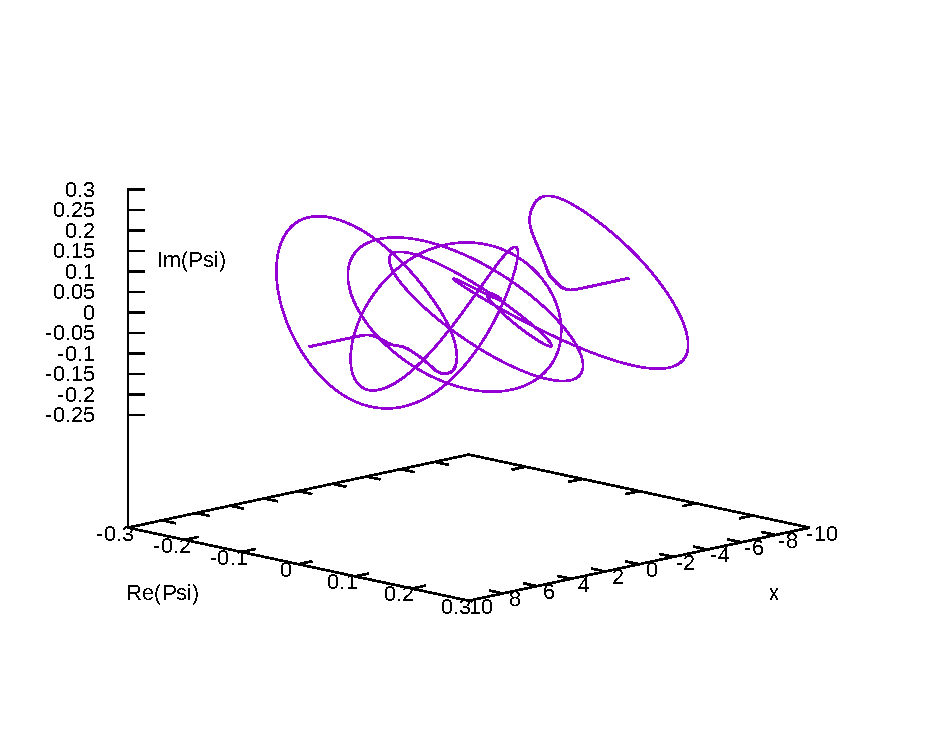
\includegraphics[width=0.7\textwidth]{plots/super-square-9-12-15-3d.pdf}
  \caption{3D plot of superposition of $V(x) = x^2$ and energies 9, 12 and 15. One can't really see anything and it's just a mess, this would be better if one could interact with the plot
  on the computer.}\label{fig:title-wave-3d}
\end{figure}
\begin{figure}[H]
  \centering
  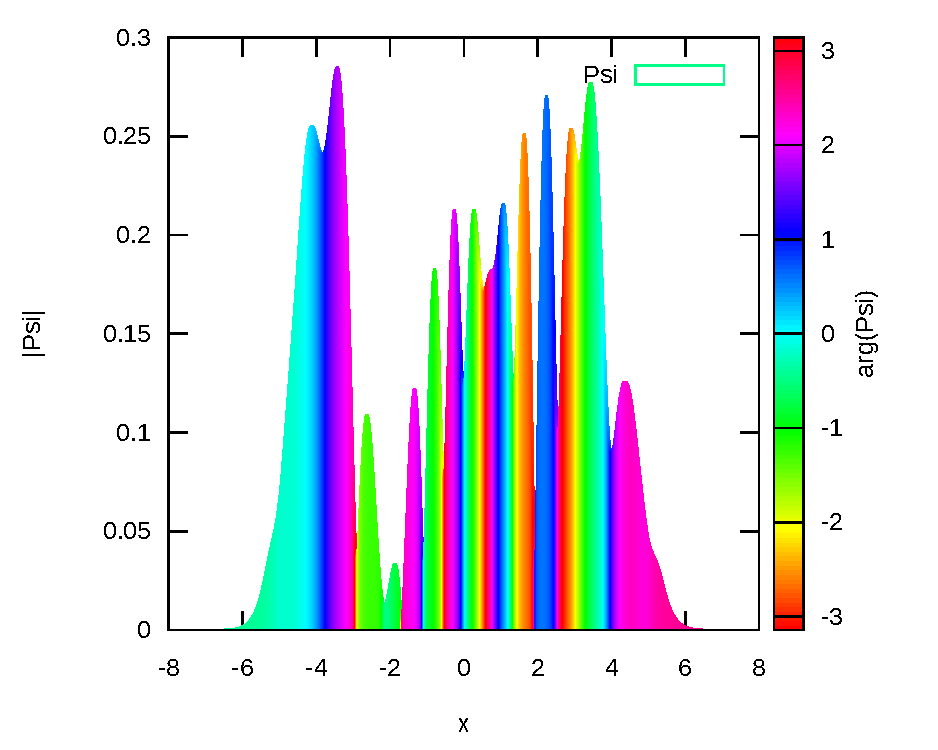
\includegraphics[width=0.7\textwidth]{plots/super-square-9-12-15-color.pdf}
  \caption{Color plot of superposition of $V(x) = x^2$ and energies 9, 12 and 15. Although it takes time to get used to, this plot is much clearer compared to figure~\ref{fig:title-wave-3d}.}
\end{figure}
As shown in figure~\ref{fig:title-wave-3d}, the 3D plot is basically unusable since there is no depth. This would usually be fixed with lighting but it would be very difficult to apply lighting on a line
such that one could actually see the depth. In the color plot everything seems to be clear, except that the values of the phase can't be read precisely.

When plotting the function yourself the author would still recommend the 3D plot because it's clearer when you can move it around.

Figure~\ref{fig:color-to-phase-circle} should help to read the color plots.
\begin{figure}[H]
  \centering
  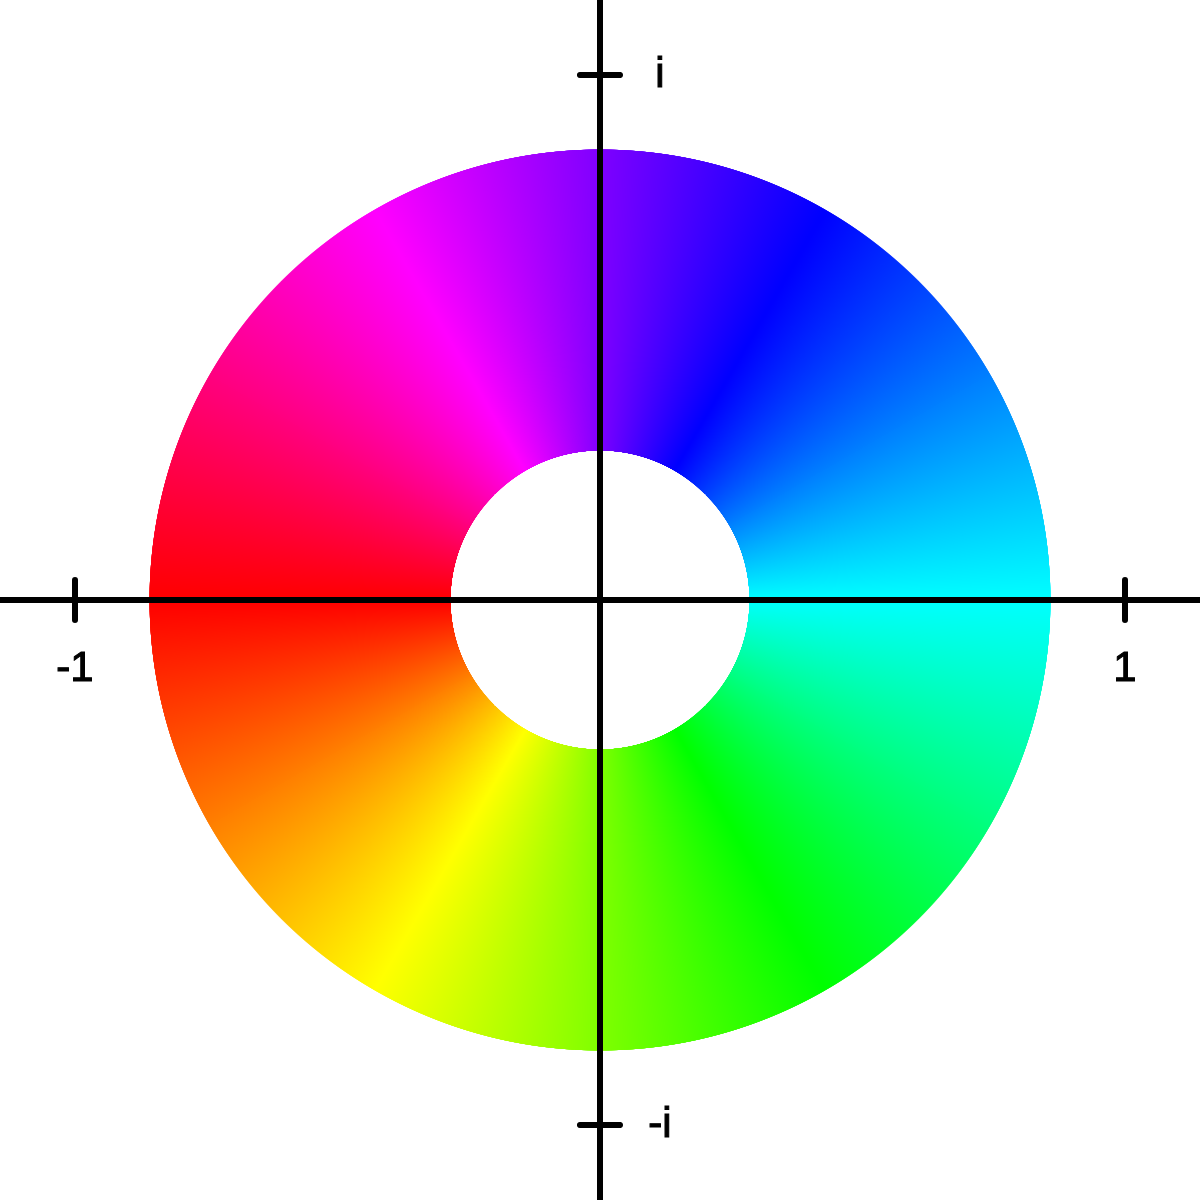
\includegraphics[width=0.8\textwidth]{plots/color_circle.png}
  \caption{Illustration of the mapping of an angle to color to represent complex numbers. Every argument of a complex number is assigned to a color.}\label{fig:color-to-phase-circle}
\end{figure}
For example $1 + 0 \mi$ would have the color cyan and $0 + 1 \mi$ would be purple.
This graph is a handy tool to read the color plots that will be used later since it's easier to associate the angle with the color if the color is actually at that angle
rather then a number in radians.

\section{Planck Units}
By using Planck units the equations get a little bit easier.
Working in Planck units means that all fundamental constants are equal to 1.
\[
  c = k_{B} = G = \hbar = 1.
\]
This means that the constants will usually cancel out.

To convert to SI units one can just multiply powers of the constants such that their unit results in one of the base units.
\begin{align*}
l_{\text{Planck}} = l_{\text{SI}} \sqrt{\cfrac{G \hbar}{c^{3}}}  && 1~\text{m}_{\text{Planck}}  \approx 1.616255(18) \cdot 10^{-35}~\text{m}  && \text{\citep{CODATAValuePlanckLength}} \\
m_{\text{Planck}} = m_{\text{SI}} \sqrt{\cfrac{c \hbar}{G}}      && 1~\text{kg}_{\text{Planck}} \approx  2.176434(24) \cdot 10^{-8}~\text{kg} && \text{\citep{CODATAValuePlanckMass}} \\
t_{\text{Planck}} = t_{\text{SI}} \sqrt{\cfrac{G \hbar}{c^{5}}} && 1~\text{s}_{\text{Planck}}  \approx 5.391247(60) \cdot 10^{-44}~\text{s}  && \text{\citep{CODATAValuePlanckTime}}
\end{align*}
\hspace*{\fill}~\citep[Table 1]{gaarder2016gravitational} \\
\\
The program will take all of its in- and outputs in Planck units.


\section{Benchmarking}
Benchmarking is the process where one tests the performance of software. In the case of \emph{schroeding\_approx} the goal would be to test the individual parts and
find out where improvements are possible, and in a later step whether the supposed improvements actually improved the performance. For this the two tools described below will be used.

\subsection{perf}
\emph{perf} is a collection of performance analysis tools for Linux~\citep{perf2022manula}. It will later be used to measure the performance of \emph{schroedinger\_approx}.
In its manual page \citep{perf2022manula} it's described as:
\begin{quoting}
Performance counters for Linux are a new kernel-based subsystem that provide a framework for all things performance analysis. It covers hardware level (CPU/PMU, Performance Monitoring Unit) features and software features (software counters, tracepoints) as well.
\end{quoting}
In particular, \bashinline{perf stat} and \bashinline{perf record} will be used.
\\[3ex]
The outputs produced by \bashinline{perf stat} are fairly technical and can measure performance on the CPU level.
Most of the metrics produced \emph{will not} be used. An example reproduced of a benchmark of \emph{schroedinger\_approx} is reproduced below.

\begin{minipage}{\textwidth}
    \begin{lstlisting}
            727,840.51 msec task-clock                       #   15.452 CPUs utilized
            404,803      context-switches                 #  556.170 /sec
                5,210      cpu-migrations                   #    7.158 /sec
                30,529      page-faults                      #   41.945 /sec
    2,482,025,824,794      cycles                           #    3.410 GHz
        1,855,377,839      stalled-cycles-frontend          #    0.07% frontend cycles idle
        3,495,430,962      stalled-cycles-backend           #    0.14% backend cycles idle
    4,704,001,143,909      instructions                     #    1.90  insn per cycle
                                                    #    0.00  stalled cycles per insn
    566,687,255,541      branches                         #  778.587 M/sec
        252,663,255      branch-misses                    #    0.04% of all branches

        47.103191946 seconds time elapsed

        722.481191000 seconds user
        5.147335000 seconds sys
    \end{lstlisting}
    \begin{description}
      \item[CPUs utilized] This states how many percent of the \emph{CPU} were actually used, important to note is that ``CPU'' in this case means hardware thread. In the case of the test machine, it
            has 8 cores with 2 threads each, therefore in theory this number could be as high as 16.0. The goal would be to use as much of the CPU as possible but one has to be cautious because other
            processes besides \emph{schroedinger\_approx} are also running and use some part of the CPU.

      \item[context-switches] This factor is handled by the Linux kernel. The kernel \emph{switches} between processes that can run on a thread of the CPU. In this case most of the context switches were
            happening inside \emph{schroedinger\_approx} itself because behind the scene it uses a thread pool. In general it is an indicator of how efficiently the kernel can handle the multi threading in
            a program.
      \item[page-faults] This is an ``error'' that happens inside the CPU when a process is trying to access memory that is not yet loaded into the cache of the CPU. When the number of page faults per
            second is high, the process's memory layout is not good and should be optimized. Such optimizations are very hard to do.

      \item[branch-misses] Modern CPUs don't actually execute the assembly directly but they perform \emph{speculative execution}. This means the CPU ``guesses'' ahead if for example an if-statement will
            be true and then already do the calculations before the instruction pointer actually reached the branch. Even though the CPU is pretty good at ``guessing'', if it's wrong it has to throw away
            all those calculation; this is called a \emph{branch miss}. The code can be made faster if the percentage of branch misses is low (< 0.05\%). this can be done by writing ``predictable'' code
            which requires intensive testing.
      \item[time elapsed] This is the time the program was running. This is similar to the \bashinline{time} command.

    \end{description}
\end{minipage}



\subsection{Rust Benchmarks}
The nightly version of Rust contains benchmarks that can be run with the command \bashinline{cargo bench}. The benchmarks are the functions marked with the \rustinline{#[bench]} macro. All those functions take a \rustinline{test::Bencher} as an argument.
This struct will measure the time it takes the code to complete. It will also run the fragments multiple times. Finlay it will print the time measurements for each benchmark to the terminal.

While \emph{perf} captures the big picture, it's possible to \emph{zoom} in to the individual components of the system with Rust benchmarks.

\chapter{Methods}\label{chap:methods}
This chapter is about the implementation details and which algorithms and mathematics are used behind the scenes. Some smaller details of the code will not be discussed.

\section{Program Architecture}
The program has multiple interfaces, or traits as they are called in Rust, that give the program some abstraction.
In Appendix~\ref{fig:uml-arch} is a diagram of the architecture.
Since the current version of Rust does not support manual implementations of \rustinline{std::ops::Fn} a custom trait will be defined for functions \rustinline{Func<A, R>} where \rustinline{A} is the type
of the argument and \rustinline{R} is the return type. Later this trait will be used to implement functions for integration, evaluation and more utilities.

The \rustinline{WaveFunction} struct is at the heart of the program, as it contains all the functionality to build wave functions. It is composed of \rustinline{WaveFunctionPart} which represent either a
\rustinline{Joint}, \rustinline{PureWkb} or an \rustinline{ApproxPart} which will be discussed in detail in section~\ref{sec:wave-func-parts}. With the \rustinline{range} function it can be checked when a
part is valid, that is to say, when it can be evaluated without a large error.

\section{Newton's Method}
Newton's method, also called the Newton-Raphson method, is a root-finding algorithm that uses the first few terms of the Taylor series of a function $f(x)$ in the vicinity of a suspected root
\citep{math:newton}. It makes a sequence of approximations of a root $x_{n}$ that in certain cases converges to the exact value where
\[
  \lim _{n \to \infty}f(x_{n}) = 0.
\]
\\
The sequence needs a first guess of where the root could be which will be the variable $a$, then the sequence is defined as
\begin{align*}
  x_{0}=a \\*
  x_{n+1}=x_{n}-\cfrac{f(x_{n})}{f'(x_{n})}.
\end{align*}
Visually this looks like figure~\ref{fig:newton-ilust} where $f(x) = (x-2)(x-1)(x+1)$ was taken as an example.
\begin{figure}[H]
	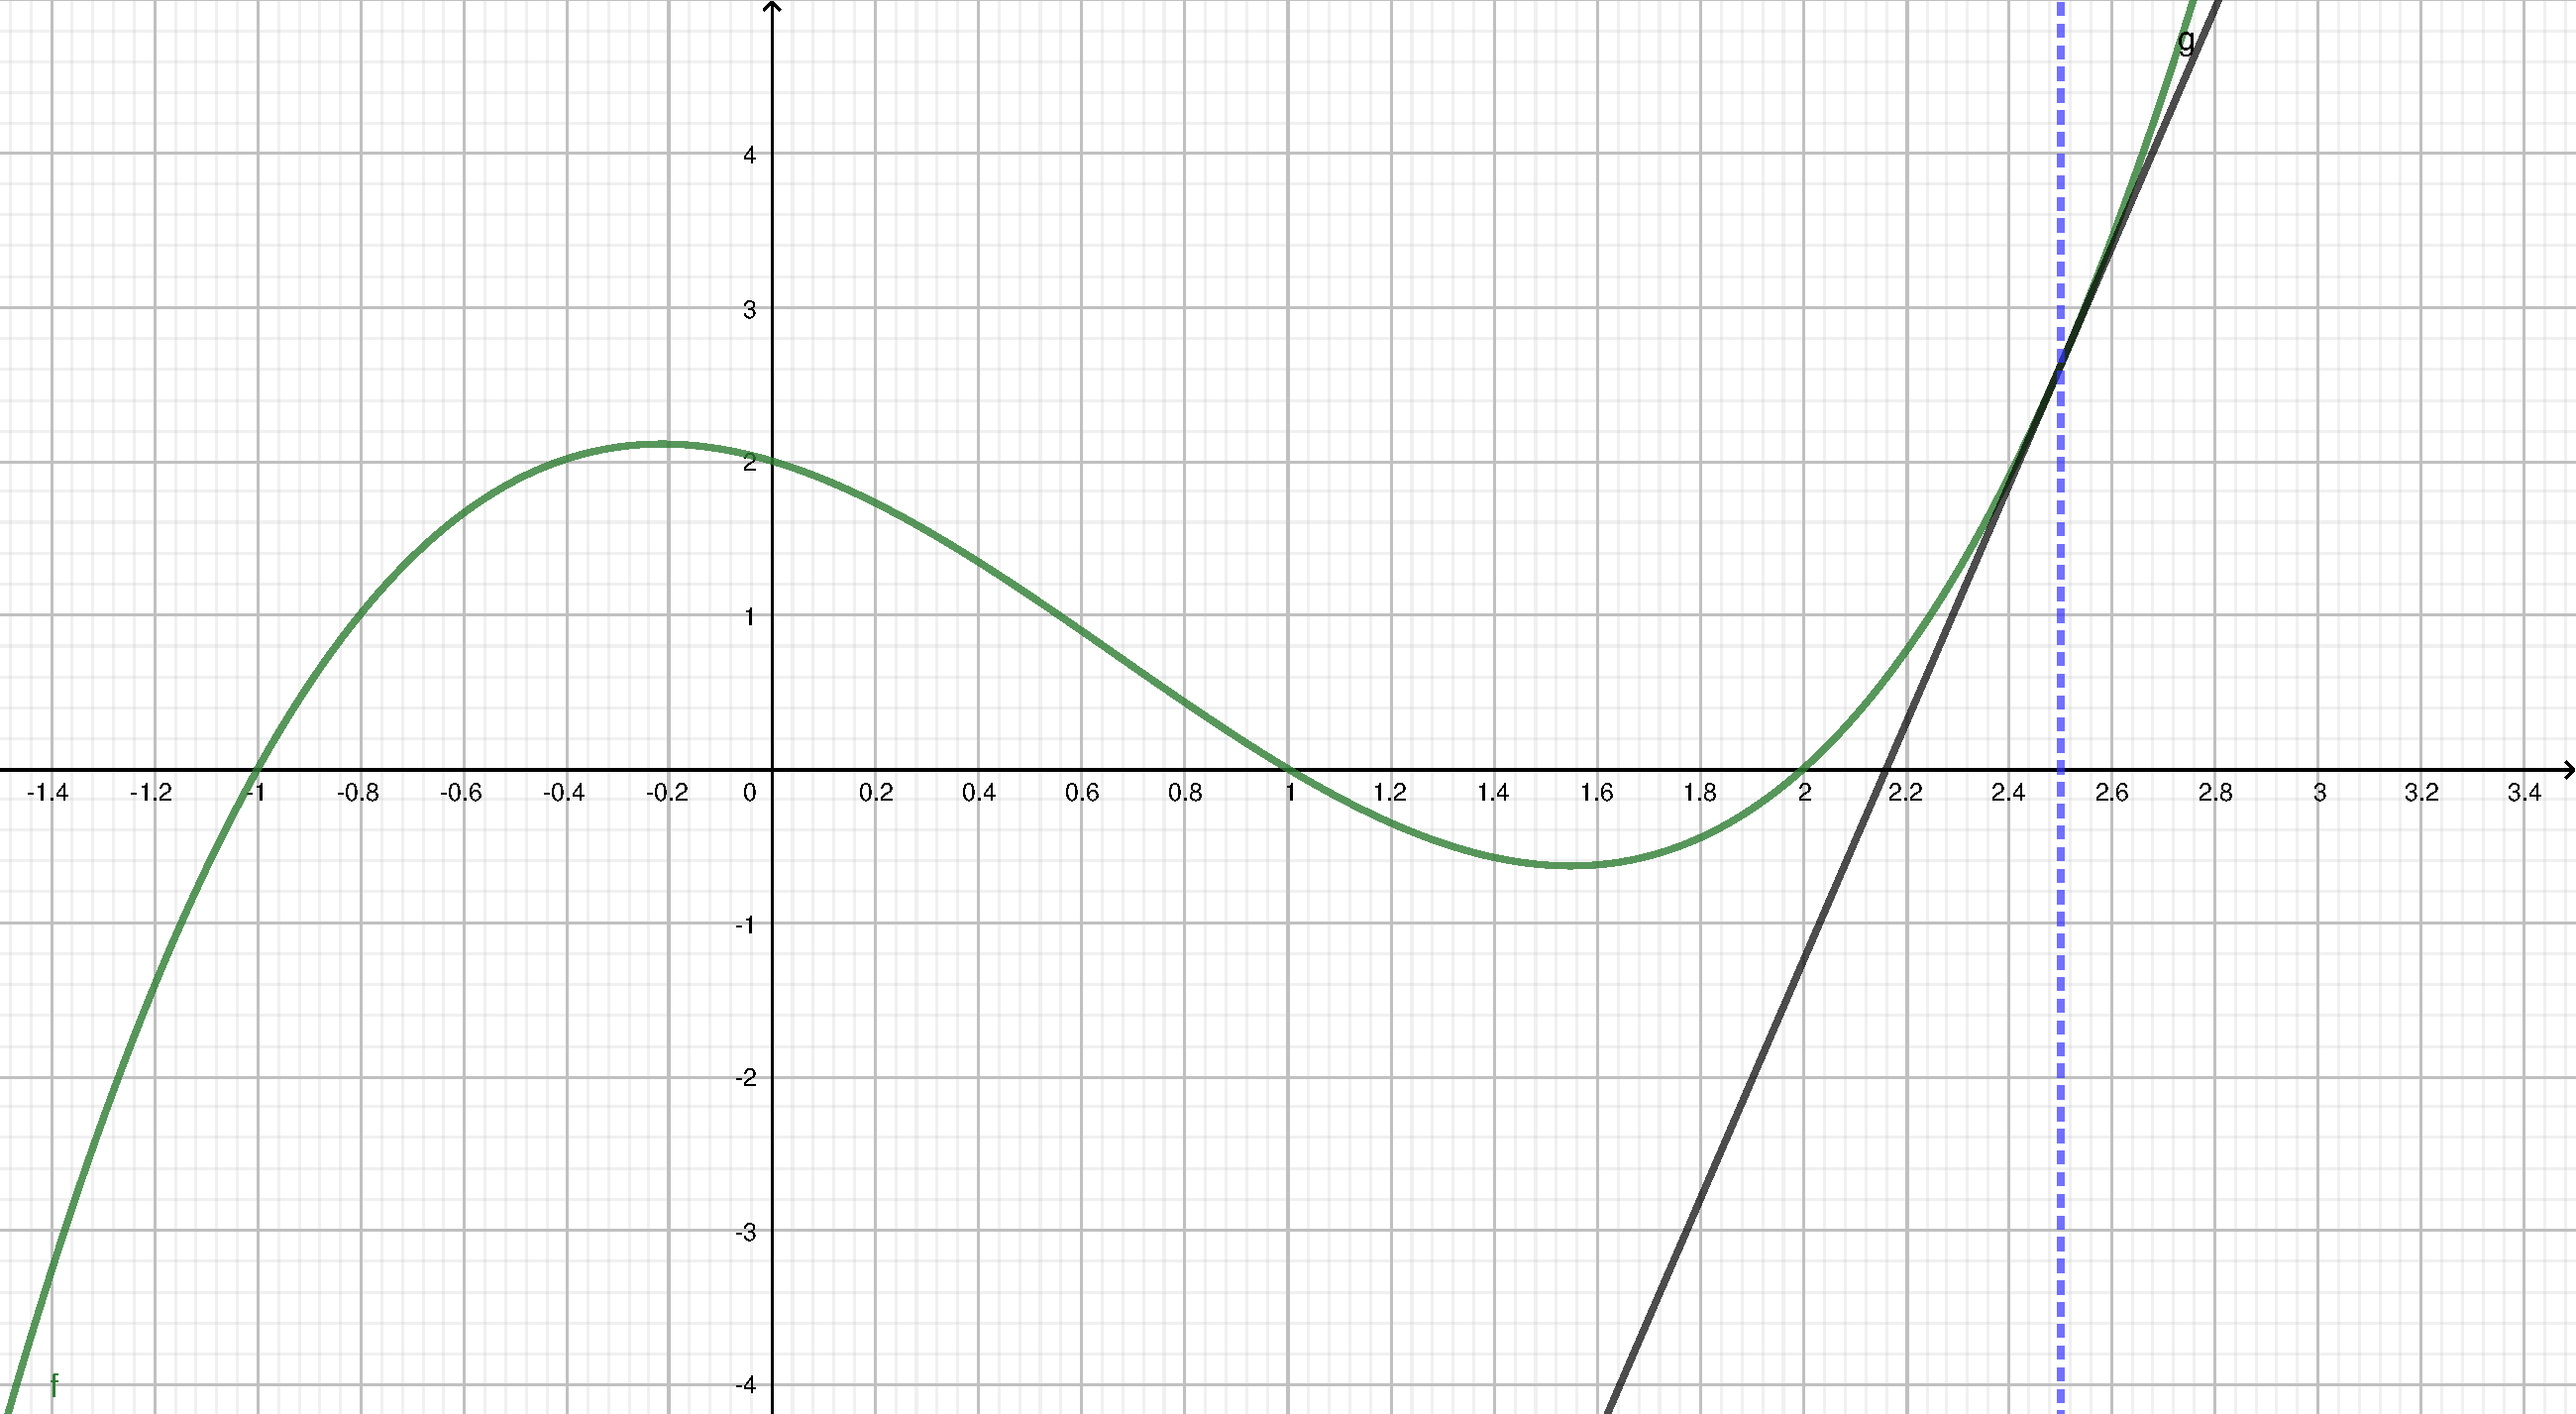
\includegraphics[width=\textwidth]{plots/newtons-method.pdf}
	\caption{Illustration of Newton's method, $f(x) = (x-1)(x-2)(x+1)$.The blue line indicates the initial guess which in this case is $2.5$. The black line ($g(x)$) is a tangent to $f(x)$ at
      $(guess, f(guess))$, the next guess will be where the tangent intersects the x-axis (solution of $g(x) = 0$). This converges more quickly then other methods such as Regula falsi}
	\label{fig:newton-ilust}
\end{figure}
.

\begin{rustcode}[label=code:newtons-method, caption={
Implementation of Newton's method. The function takes a closure \rustinline{f}, the initial guess \rustinline{guess} and a stop condition \rustinline{precision}.
The function will return if $\left|{f(x_{n})}~/~{f'(x_{n})}\right|$ is less than \rustinline{precision}. If the derivative at any point becomes $0$ the function will panic. Because of this the function
\rustinline{newtons_method_max_iters} provides an alternate implementation that will not panic and \emph{always} return an \rustinline{Option}.
}]
pub fn newtons_method<F>(f: &F, mut guess: f64, precision: f64) -> f64
where
    F: Fn(f64) -> f64,
{
    loop {
        let deriv = derivative(f, guess);

        if deriv == 0.0 {
            panic!("Devision by zero");
        }

        let step = f(guess) / deriv;
        if step.abs() < precision {
            return guess;
        } else {
            guess -= step;
        }
    }
}
\end{rustcode}

An extension to the function in snippet~\ref{code:newtons-method} is implemented in the struct \rustinline{Newton'sMethodFindNewZero} which can be used to find multiple roots.

From the structure of the algorithm it is tempting to implement it recursively, but using a loop is much faster since there are no unnecessary function calls and the precision can (at least in
theory) be $0$ without causing a stack overflow.

\section{Regula Falsi with Bisection}
Newton's method fails if the first guess is at a maximum, since the step would go to infinity. For these cases a bisection method will be applied until the sign of the function changes.
This needs to done because Regula Falsi requires two guesses.

The algorithm itself is quite simple. To start define the parameters
\begin{align}
  f(x): \mathbb{R} \to \mathbb{R} \\
  \{a \in \mathbb{R}~|~f(a) \le 0\} \\
  \{b \in \mathbb{R}~|~f(b) \ge 0\}.
\end{align}
Then draw a line between the two points $(a, f(a))$ and $(b, f(b))$. Then $b$ becomes
the x-value where the line intersects the x-axis, when this process is applied
again with the new $b$ the resulting value will become the new $a$. This process can be
repeated until a fresh hold is crossed for the accuracy and the result will be the last intersection of the line with the x-axis.

\section{Derivatives}
Derivatives can be calculated numerically as in the C++ library Boost \citep{boost:calculating-derivative}.
The author implemented a analytical system for calculating derivatives in Go. This project used an interface with two methods: \rustinline{function} and \rustinline{derivative}. Afterwards functions for
operations like multiplication, addition, etc. were added. In these operations the function's derivative was built based on the operation. This process of writing functions is tedious and the performance
is worse than in the numerical implementation in rust (snippet~\ref{code:derivative}).

\begin{minipage}{\textwidth}
\begin{rustcode}[label=code:derivative, caption={
Rewrite of the C++ library Boost's implementation \citep{boost:calculating-derivative} of numerical differentiation for Rust.
\rustinline{f64::epsilon().sqrt()} is approximately $1.4901161\cdot 10^{-8}$.
\rustinline{f64::epsilon()} is the smallest double precision floating point number $\epsilon$ where $1 +
\epsilon \ne 1$. This value has been chosen for $dx$ because it is precise enough.
}]
pub fn derivative<F, R>(func: &F, x: f64) -> R
where
    F: Fn(f64) -> R + ?Sized,
    R: Sub<R, Output = R> + Div<f64, Output = R> + Mul<f64, Output = R> + Add<R, Output = R>,
{
    let dx = f64::epsilon().sqrt();
    let dx1 = dx;
    let dx2 = dx1 * 2.0;
    let dx3 = dx1 * 3.0;

    let m1 = (func(x + dx1) - func(x - dx1)) / 2.0;
    let m2 = (func(x + dx2) - func(x - dx2)) / 4.0;
    let m3 = (func(x + dx3) - func(x - dx3)) / 6.0;

    let fifteen_m1 = m1 * 15.0;
    let six_m2 = m2 * 6.0;
    let ten_dx1 = dx1 * 10.0;

    return ((fifteen_m1 - six_m2) + m3) / ten_dx1;
}
\end{rustcode}
\end{minipage}

\section{Integration}
The same principles apply to integrals as to derivatives, and so it wouldn't be a great benefit to
implement an analytic integration system. Integrals would also be much more difficult to
implement than derivatives since integrals can not be broken down into many smaller
integrals that can be computed easily. Instead it would have to be solved as is.

One approach would be to use the same method as with the derivative, take the definition with the limit and use a small value. But this method can be improved: since integrals calculate
areas under curves a trapeze is more efficient and accurate than the rectangle that results
from the definition.

\begin{figure}[h]
  \centering
	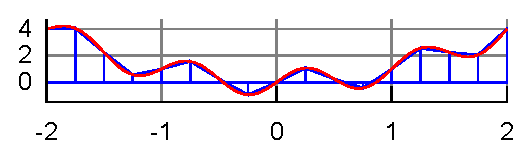
\includegraphics[width=0.7\textwidth]{plots/Integration_trapezoid.pdf}
	\caption{Illustration of integration with trapeze from \cite{wiki:integration-methods}.}
	\label{fig:integration-ilust}
\end{figure}

Figure~\ref{fig:integration-ilust} shows visually how the methods work, each blue trapeze has an area of
\[
\int _{a}^{b}f(x)\,dx\approx (b-a)f\left({\cfrac {a+b}{2}}\right).
\]
where $a$ and $b$ are the bounds of integration. One trapeze would be fairly inaccurate to calculate the area under the function, but as the area from $a$ to $b$ is subdivided further the approximation
generally gets better.

The general structure of the algorithm can very easily be run in parallel since it doesn't matter in which order the segments are added together and the segments also don't dependent on one another.
In Rust this is implemented using \emph{rayon}. \emph{rayon} is an implementation for parallel iterators meaning that normal data structures that implement \rustinline{std::iter} can be run in parallel
\emph{just} by changing \rustinline{::iter()} to \rustinline{::par_iter()}~\citep{rayonreadme}. While programing the author noticed that this does not work in all cases and the compiler would throw an
error because certain objects can't be shared across threads. In particular the objects have to implement the \rustinline{Send} and \rustinline{Sync} traits \citep{rustlang2022nomicon}.

The implementation of the integral approximation consists of two functions as shown in code snippet~\ref{code:evaluate_function_between} and \ref{code:integrate}.

\begin{rustcode}[caption = {
    \rustinline{Point} stores both the input x and the output y of a function
    and In order functions with states, like wave functions that store parameters, can be integrated,
    there is a trait \rustinline{Func<A, R>}. The \rustinline{evaluate_function_between} then evaluates the function \rustinline{f} in the interval $(a,b)$ in parallel.
    The type bonds of the function assure that as many data types of \rustinline{X} and \rustinline{Y} can be calculated.
    This function is used to implement the actual integration and to evaluate the points of the wave function.
  }, label = code:evaluate_function_between]
pub trait Func<A, R>: Sync + Send {
    fn eval(&self, x: A) -> R;
}

pub struct Point {
    pub x: f64,
    pub y: Complex64,
}

// ...

pub fn evaluate_function_between<X, Y>(f: &dyn Func<X, Y>, a: X, b: X, n: usize) -> Vec<Point<X, Y>>
where
    X: Copy
        + Send
        + Sync
        + std::cmp::PartialEq
        + From<f64>
        + std::ops::Add<Output = X>
        + std::ops::Sub<Output = X>
        + std::ops::Mul<Output = X>
        + std::ops::Div<Output = X>,
    Y: Send + Sync,
{
    if a == b {
        return vec![];
    }

    (0..n)
        .into_par_iter()
        .map(|i| {
            index_to_range(
                X::from(i as f64),
                X::from(0.0_f64),
                X::from((n - 1) as f64),
                a,
                b,
            )
        })
        .map(|x: X| Point { x, y: f.eval(x) })
        .collect()
}
\end{rustcode}

\begin{rustcode}[caption = {
The actual integration happens in \rustinline{integrate}, which calculates the areas of the trapezes between the points passed to it. For optimization 1000 trapezes are calculated per thread because it
would take more time to create a new thread than to actually do the calculation, these 1000 values are called a \emph{batch}.
This parameter was chosen for the author's computer and 1000 might not be optimal for all CPUs.
After all batches have been calculated the boundaries between batches also have to be considered therefore they are added in the end with \rustinline{rest}.
    }, label=code:integrate]
pub fn integrate<
    X: Sync + std::ops::Add<Output = X> + std::ops::Sub<Output = X> + Copy,
    Y: Default
        + Sync
        + std::ops::AddAssign
        + std::ops::Div<f64, Output = Y>
        + std::ops::Mul<Output = Y>
        + std::ops::Add<Output = Y>
        + Send
        + std::iter::Sum<Y>
        + Copy
        + From<X>,
>(
    points: Vec<Point<X, Y>>,
    batch_size: usize,
) -> Y {
    if points.len() < 2 {
        return Y::default();
    }

    let batches: Vec<&[Point<X, Y>]> = points.chunks(batch_size).collect();

    let parallel: Y = batches
        .par_iter()
        .map(|batch| {
            let mut sum = Y::default();
            for i in 0..(batch.len() - 1) {
                sum += trapezoidal_approx(&batch[i], &batch[i + 1]);
            }
            return sum;
        })
        .sum();

    let mut rest = Y::default();

    for i in 0..batches.len() - 1 {
        rest += trapezoidal_approx(&batches[i][batches[i].len() - 1], &batches[i + 1][0]);
    }

    return parallel + rest;
}
\end{rustcode}


\section{Transition Regions}
The approximation that will be used splits $\Psi(x)$ into multiple parts that do not match perfectly together.

\begin{figure}[h]
  \centering
  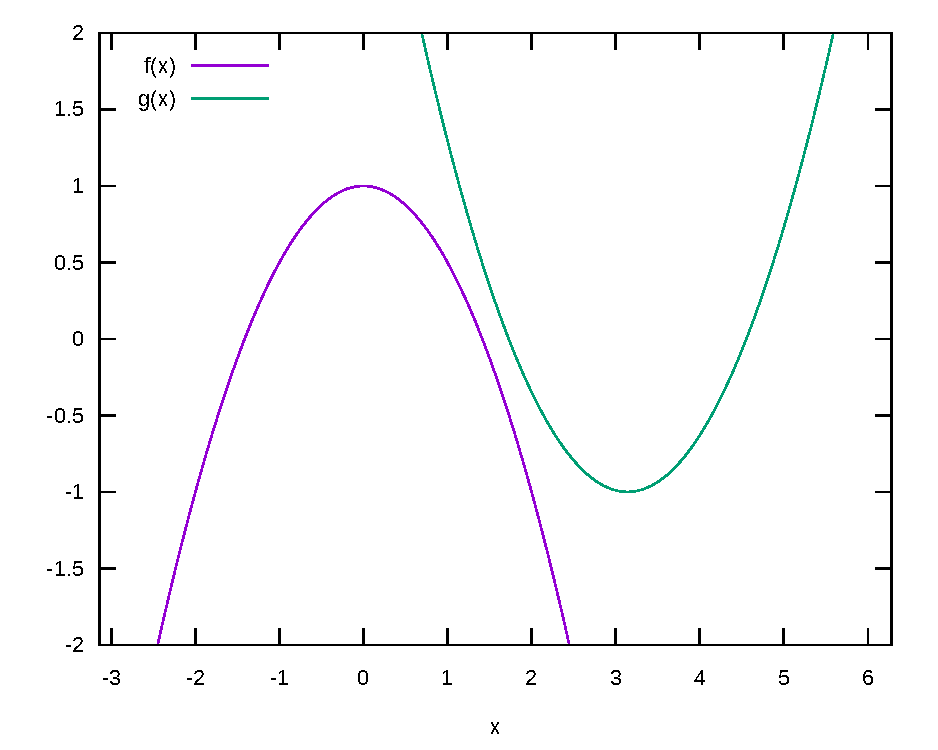
\includegraphics[width=.9\textwidth]{plots/cos_taylor.pdf}
  \caption{Two example functions that should be joined at $x=\frac{\pi}{2}$. The functions are two Taylor series of cosine, they have been chosen as an example because they don't overlap and get
  close together at $x = \frac{\pi}{2}.$}\label{fig:cos_taylor}
\end{figure}

Lets consider an example, in figure \ref{fig:cos_taylor} we can see two Taylor series of cosine. Now the two functions have to be joined at $x = \pi / 2$ in such a way that it's a mathematically smooth transition.
\begin{align}
  \label{joint:f}
  f(x) = 1 - \cfrac{x^{2}}{2} \\
  \label{joint:g}
  g(x) = \cfrac{(x - \pi)^{2}}{2} -  1
\end{align}

As a first guess let's join $f(x)$ and $g(x)$ with a step function, this means that the joint function $h(x)$ will be
\[
  h(x) =  \left\{
    \begin{array}{ll}
           f(x) & x < \cfrac{\pi}{2} \\
           g(x) & x > \cfrac{\pi}{2}
    \end{array}
    \right..
\]
This results in figure~\ref{fig:joint-step} which is obviously not smooth.
\begin{figure}[H]
  \centering
  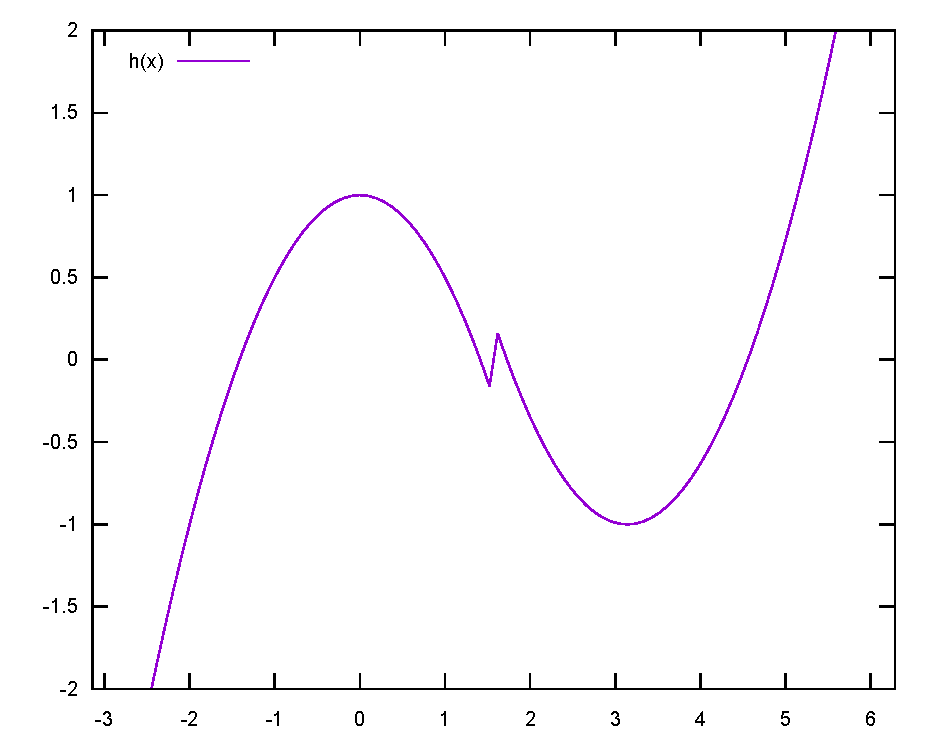
\includegraphics[width=.9\textwidth]{plots/step_joint.pdf}
  \caption{Plot of h(x) with step joint. As shown the transition is not smooth and there's a discontinuity at $x = \frac{\pi}{2}$.}\label{fig:joint-step}
\end{figure}

Using the formula from~\cite[p. 325, section 15.6.4]{hall2013quantum}
\begin{align*}
    \delta = 0.5 \\
    \alpha = \cfrac{\pi}{2} - \cfrac{\delta}{2} \\
    \chi(x) = \sin^{2}\left(x \cfrac{\pi}{2}\right)
\end{align*}
a much better result can be obtained:
\[
  h(x) =  \left\{
    \begin{array}{ll}
      f(x) & x < \alpha \\
      g(x) & x > \alpha + \delta \\
      f(x) + (g(x) - f(x))\chi(\cfrac{x-\alpha}{\delta}) & else
    \end{array}
    \right.
\]
which is mathematically smooth as can be seen in figure~\ref{fig:joint-cos-hall} (proof in Appendix~\ref{proof:joint}).
\begin{figure}[H]
  \centering
  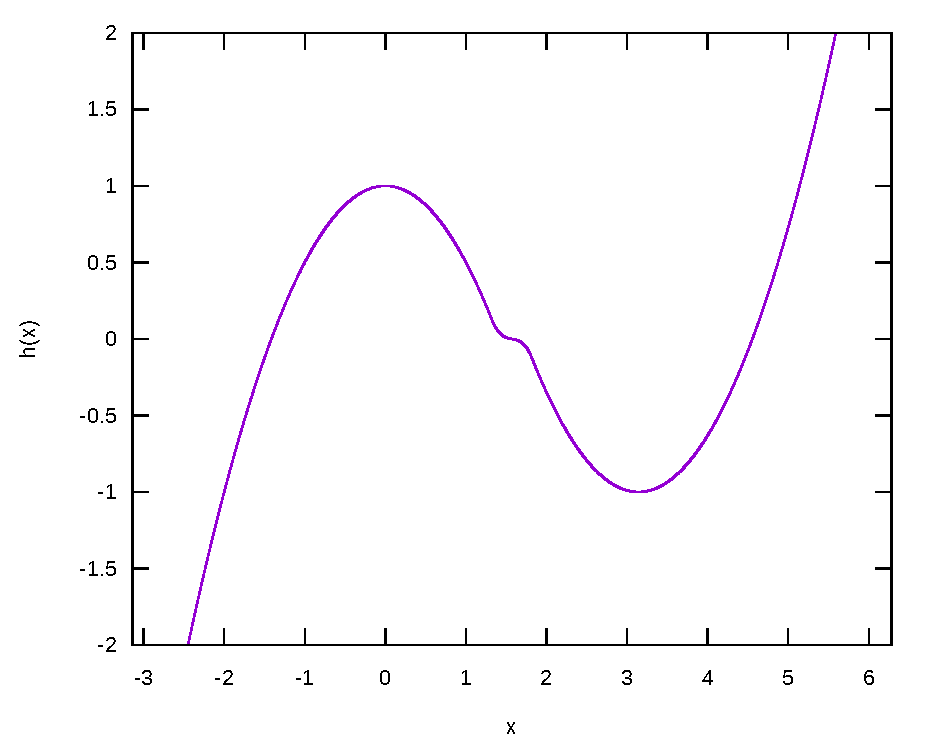
\includegraphics[width=.9\textwidth]{plots/hall_joint.pdf}
  \caption{Plot of h(x) with Hall joint. The function is smooth and has a slight \emph{bump} at $x = \frac{\pi}{2}$}\label{fig:joint-cos-hall}
\end{figure}

\subsection{Implementation in Rust}
In the program the struct \rustinline{Joint} implements the formula from \cite{hall2013quantum}.
As in the example the two functions $f(x)$ and $g(x)$, which will be renamed to \rustinline{left} and \rustinline{right}, have to be joined at $\alpha$ over a range of $\delta$. The variables $\alpha$ and $\delta$ are from now on called \rustinline{cut} and \rustinline{delta}.
\begin{rustcode}
#[derive(Clone)]
pub struct Joint {
    pub left: Arc<dyn Func<f64, Complex64>>,
    pub right: Arc<dyn Func<f64, Complex64>>,
    pub cut: f64,
    pub delta: f64,
}

impl Func<f64, Complex64> for Joint {
    fn eval(&self, x: f64) -> Complex64 {
        let chi = |x: f64| f64::sin(x * f64::consts::PI / 2.0).powi(2);
        let left_val = left.eval(x);
        return left_val + (right.eval(x) - left_val) * chi((x - self.cut) / self.delta)
    }
}
\end{rustcode}

In the proof it has been assumed that $f(x)$ and $g(x)$ are continuous of first order in the interval $(\alpha, \alpha + \delta)$. In the code this assumption will not be checked, since it would have a major impact on performance to check the derivative on every point.

\chapter{Calculation}
In this chapter discusses the calculations in the program utilizing the methods described in chapter~\ref{chap:methods}.
\section{Energy Levels}\label{sec:energy-calculation}
Solving the Schrödinger equation is an eigenvalue problem. This means that only certain energies will result in physically correct results. For an energy to be valid it has to satisfy the condition described by \cite[eq. 15.31]{hall2013quantum}.
\begin{align}
  n \in \mathbb{N}_{0}\\
  C = \left\{x \in \mathbb{R}~|~V(x) < E \right\}\\
  \int_{C}\sqrt{2m(E - V(x))}dx = \pi(n + 1/2)\label{eq:energy-cond}
\end{align}
where $C$ is the set of all values for $x$ in the classically allowed region, $m$ the mass, $V(x)$ the potential and $E$ the energy of the particle. $n$ is used to specify which energy level should be
calculated. It can be interpreted such that the oscillating part of the wave function has to involve only complete or half oscillations. \cite{hall2013quantum} also states that the equations from
section~\ref{meth:wkb:approximation-scheme} have to agree, up to multiplication by a constant which will be the case iff equation~\ref{eq:energy-cond} is satisfied.

To solve this problem for an arbitrary potential in a computer, the condition can be rewritten to equation~\ref{eq:prog_cond} such that the implementation is easier on a computer.
\begin{align}
  p(x) = \left\{\begin{array}{ll}
                  \sqrt{2m(E - V(x))} & V(x) < E \\
                  0 & else
                \end{array}
                      \right. \\\label{eq:prog_cond}
  \cfrac{2 \int_{-\infty}^{\infty}p(x) dx - \pi}{2\pi} \mod{1} = 0
\end{align}
where $p(x)$ is the momentum, $m$ the mass, $V(x)$ the potential and $E$ the energy of the particle.
Because~\ref{eq:prog_cond} is not continuous, Newton's method can't be applied. Furthermore the bounds of integration have to be finite, this means the user of the program will have to
specify a value for the constant \rustinline{APPROX_INF} where any value for $x$ outside of that range should satisfy $V(x) > E$. But it shouldn't be to big since the \rustinline{integrate} function can only evaluate a relatively small number (default 64000) of trapezes before the performance will suffer enormously. The default value for \rustinline{APPROX_INF} is \rustinline{(-200.0, 200.0)}.

\begin{rustcode}[caption={
    The implementation checks for discontinuities as follows: the first interval \rustinline{(0.0, ENERGY_STEP)} is checked, if there are not enough zeros the next interval is checked. This is repeated until $n$ zeros have been found.
It's also possible that equation~\ref{eq:prog_cond} is negative before the 0th energy, therefore it is also checked for sign changes.
}]
pub fn nth_energy<F: Fn(f64) -> f64 + Sync>(n: usize, mass: f64, pot: &F, view: (f64, f64)) -> f64 {
    const ENERGY_STEP: f64 = 10.0;
    const CHECKS_PER_ENERGY_STEP: usize = INTEG_STEPS;
    let sommerfeld_cond = SommerfeldCond { mass, pot, view };

    let mut energy = 0.0;
    let mut i = 0;

    loop {
        let vals = evaluate_function_between(
            &sommerfeld_cond,
            energy,
            energy + ENERGY_STEP,
            CHECKS_PER_ENERGY_STEP,
        );
        let mut int_solutions = vals
            .iter()
            .zip(vals.iter().skip(1))
            .collect::<Vec<(&Point<f64, f64>, &Point<f64, f64>)>>()
            .par_iter()
            .filter(|(p1, p2)| (p1.y - p2.y).abs() > 0.5 || p1.y.signum() != p2.y.signum())
            .map(|ps| ps.1)
            .collect::<Vec<&Point<f64, f64>>>();
        int_solutions.sort_by(|p1, p2| cmp_f64(&p1.x, &p2.x));
        if i + int_solutions.len() > n {
            return int_solutions[n - i].x;
        }
        energy += ENERGY_STEP - (ENERGY_STEP / (CHECKS_PER_ENERGY_STEP as f64 + 1.0));
        i += int_solutions.len();
    }
}
\end{rustcode}

The struct \rustinline{SommerfeldCond} is a \rustinline{Func<f64, f64>} that evaluates~\ref{eq:prog_cond}.

\subsection{Accuracy}
For a benchmark the following values, will be used.
\begin{align*}
  m = 1 \\
  V(x) = x^{2} \\
  (-\infty, \infty) \approx (-200, 200).
\end{align*}
To get the actual values the \emph{Wolfram Language} with \emph{WolframScript} was used. \emph{Wolfram Language} is the programing language behind \emph{Mathematica}\footnote{State of the art technical computing program~\citep{wolfram2022description}}, it can calculate the integral analytically and precisely.
In Rust \rustinline{main} can be rewritten to code snippet~\ref{code:main-energy-calc}.
\begin{rustcode}[caption={
Main function that calculates energies 0-50 of square potential and writes the results to \bashinline{energy.txt}.
}, label=code:main-energy-calc]
fn main() {
    let output_dir = Path::new("output");

    let values = (0..=50)
        .into_iter()
        .map(|n: usize| Point::<usize, f64> {
            x: n,
            y: energy::nth_energy(n, 1.0, &potentials::square, APPROX_INF),
        })
        .collect::<Vec<Point<usize, f64>>>();

    std::env::set_current_dir(&output_dir).unwrap();
    File::create("energy.txt")
        .unwrap()
        .write_all(plot::to_gnuplot_string(values).as_bytes())
        .unwrap();
}
\end{rustcode}
The same procedure is implemented in WolframScript.
\begin{wslcode}
m = 1
V[x_] = x^2

nthEnergy[n_] = Module[{energys, energy},
    sommerfeldIntegral[en_] = Integrate[Sqrt[2*m*(en - V[x])],
                                            {x, -Sqrt[en], Sqrt[en]}]
    energys =  Solve[sommerfeldIntegral[en] == 2*Pi*(n + 1/2), en] // N;
    energy = en /. energys[[1]];
    energy
    ]

energys = Table[{n, N@nthEnergy[n]}, {n, 0, 50}]

csv = ExportString[energys, "CSV"]
csv = StringReplace[csv, "," -> " "]
Export["output/energies_exact.dat", csv]
\end{wslcode}
These programs will output two files \bashinline{energies_approx.dat}~(Appendix~\ref{dat:energy-rs}) for the implementation in Rust and \bashinline{energies_exact.dat}~(Appendix~\ref{dat:energy-wsl}) for
WolframScript. As a rough estimate an error of $\pm \cfrac{10}{64000} \approx \pm 1.56 \cdot 10^{-4}$ is expected, because the program checks for energies with that step size.

\begin{figure}[H]
  \centering
  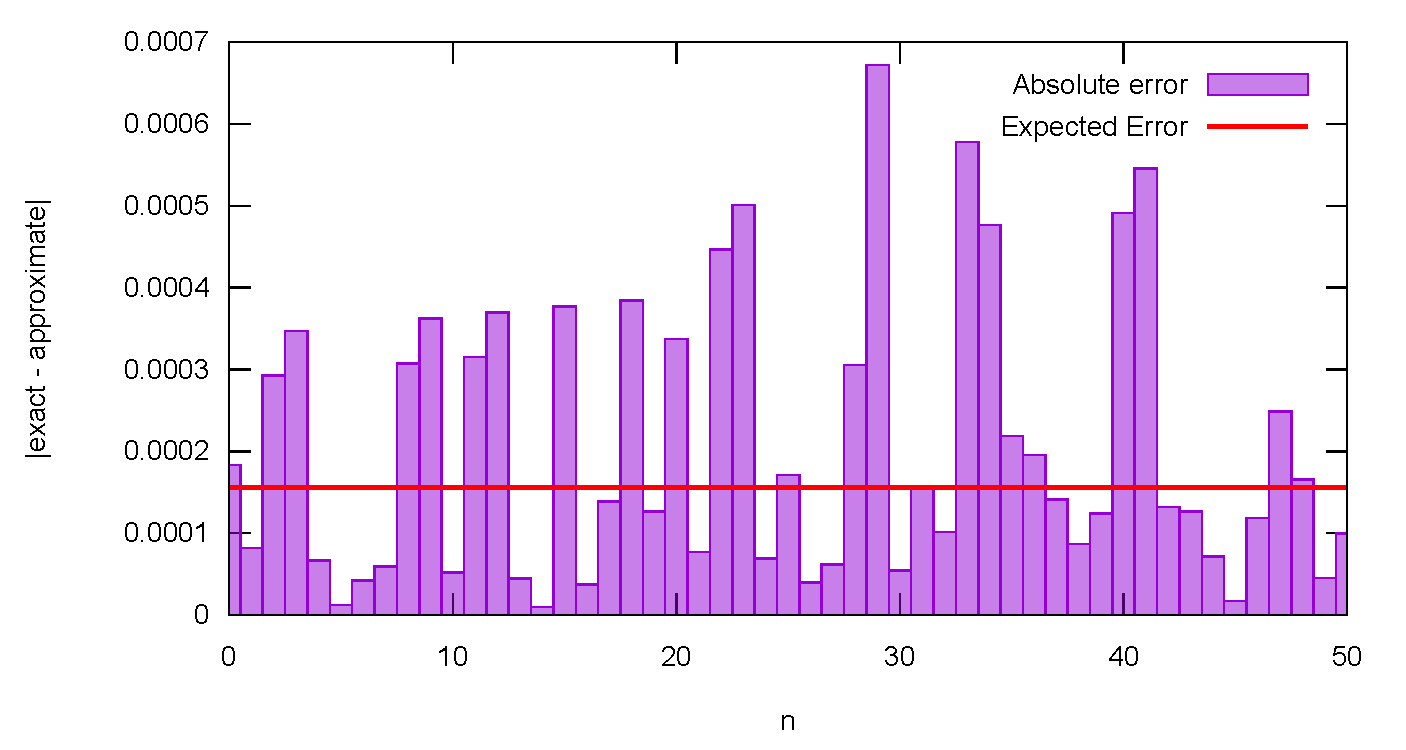
\includegraphics[width=\textwidth]{plots/energy_error.pdf}
  \caption{Absolute error of energy levels in square potential. The error is a little higher than expected which is probably due to errors in the integral. Still the algorithm should be precise
    enough.}\label{fig:energy-error}
\end{figure}
The absolute error is plotted in figure~\ref{fig:energy-error}.  It would be possible to  pick a lower value for \rustinline{ENERGY_STEP} in \bashinline{src/energy.rs:49}, but this will impact the performance for calculating energies with higher numbers for $n$.

\section{Turning Points}
A point $x$ where $V(x) = E$ is called a turning point. It is assumed that the WKB function is a good approximation in the region where
\begin{align}
  \label{eq:valid}
  -\cfrac{1}{2m} \deriv{V}{x}(x) \ll (V(x) - E)^{2}.
\end{align}
In order to do the actual calculation we need a range where the Airy function is valid.
From equation~\ref{eq:valid} it can inferred that the Airy function is valid where
\begin{align}
  \label{eq:valid-airy}
  -\cfrac{a}{2m} \deriv{V}{x}(x) - (V(x) - E)^{2} > 0
\end{align}
Further on it can assumed that the Airy function is only valid in a closed interval, which means that there must be at least two roots of equation~\ref{eq:valid-airy}. These roots will be called turning point boundaries from now on. The factor of $a$ is used to emulate the behavior of $\ll$.

The left boundary point must have a positive and the right a negative derivative. This means  after calculating the roots, they can be group together by their derivatives.
\\
In order to find all roots a modified version of Newton's method. When we find a solution $x_{0}$ we can divide the original function by $(x - x_{0})$. This means that Newton's method won't be able to find $x_{0}$ again.
\\
\label{sec:view}
To later plot the wave function we will define the so-called ``view''. This is the interval which the user has to see in the end.
It is defined to be
\begin{align*}
  t_{l} < t_{r} \\
  \left(t_{l} - f_{view} (t_{r} - t_{l}), t_{r} - f_{view} (t_{r} - t_{l})\right)
\end{align*}
where $t_{l}$ is the left- and $t_{r}$ the rightmost turning point. $f_{view}$ is a user defined constant.
These two points will be calculated by applying Newton's method to $V(x) - E$ with initial guesses at \rustinline{APPROX_INF}.

Further on since we check for roots inside the interval of the view, we don't
have a good first guess where the turning point might be. Because of this we will make $1000$
guesses evenly distributed over the interval and invent an algorithm that can rate how good of a guess a point could be.
Newton's method works well if the value of $f(x)$ is small and $f'(x)$ is neither too small nor too big.
As a rating function
\[
  \label{eq:rating-newton}
  \sigma(x) = \cfrac{|f(x)| }{ -\exp\left({{\left(\deriv{f}{x}(x)\right)}^{2} + 1}\right)}
\]
is used, where lower is better. This function is just an educated guess, but there are some properties it has to have. In particular, as the derivative of $f$ tends to 0, $\sigma(x)$ should diverge to infinity.
\[\lim_{\deriv{f}{x} \to 0} \sigma(x) = \infty\]
If $f(x) = 0$ found an actual root has been found in the first guess meaning that $\sigma(x)$
should be 0. Formula~\ref{eq:rating-newton} doesn't satisfy this property since it's
undefined if $f'(x) = 0$ and $f(x) = 0$, but the definition can be extended
\[
  \sigma(x) = \left\{
    \begin{array}{ll}
    \cfrac{|f(x)| }{ -\exp\left({{\left(\deriv{f}{x}(x)\right)}^{2} + 1}\right)} & \text{if} ~f(x) \ne 0~\text{and}~\deriv{f}{x} \ne 0 \\
    0 & \text{else}
    \end{array}\right.
\]

\begin{figure}[H]
  \centering
  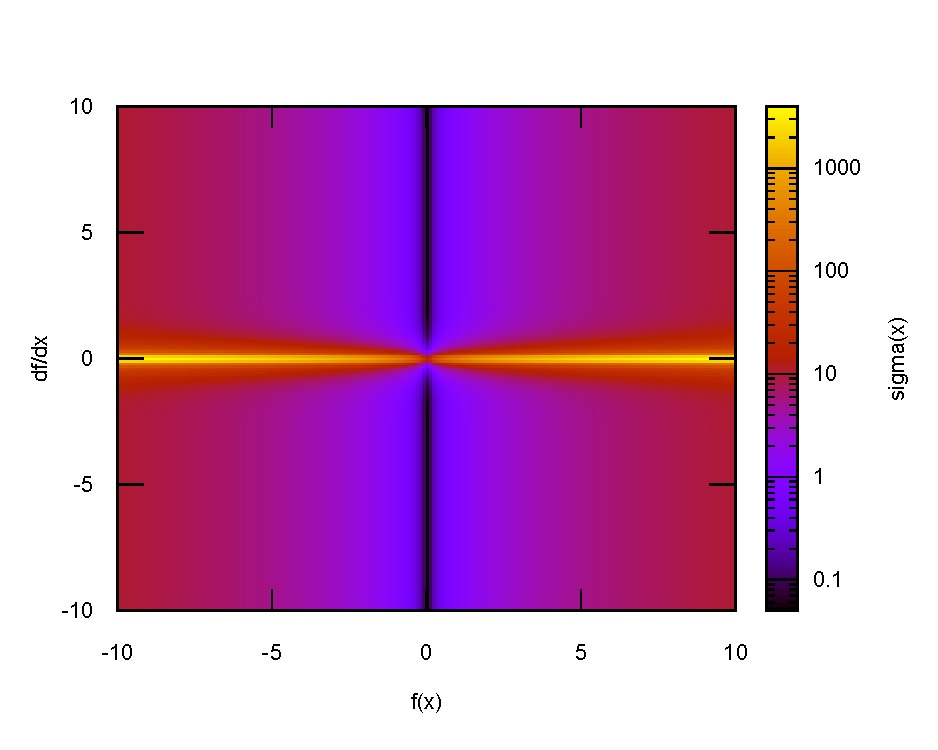
\includegraphics[width=0.9\textwidth]{plots/newton_rating_func.pdf}
  \caption{Logarithmic heat diagram of $\sigma(x)$, darker/bluer is better}\label{fig:simga-heat}
\end{figure}
As we can see in figure~\ref{fig:simga-heat} where darker/bluer values are better than yellow/red areas, $\sigma(x)$ indeed has all of the desired properties.
\\
After we rated all, of the 1000 guesses we can pick the best one as a first guess and use the modified Newton's method with it. We do this process 256 times by default. In theory we could therefore use the WKB approximation for potentials with up to 256 turning points.

\begin{rustcode}
fn find_zeros(phase: &Phase, view: (f64, f64)) -> Vec<f64> {
    let phase_clone = phase.clone();
    let validity_func = Arc::new(move |x: f64| {
        1.0 / (2.0 * phase_clone.mass).sqrt() * derivative(&|t| (phase_clone.potential)(t), x).abs()
            - ((phase_clone.potential)(x) - phase_clone.energy).pow(2)
    });
    let mut zeros = Newton'sMethodFindNewZero::new(validity_func, ACCURACY, 1e4 as usize);

    (0..MAX_TURNING_POINTS).into_iter().for_each(|_| {
        let modified_func = |x| zeros.modified_func(x);

        let guess = make_guess(&modified_func, view, 1000);
        guess.map(|g| zeros.next_zero(g));
    });

    let view = if view.0 < view.1 {
        view
    } else {
        (view.1, view.0)
    };
    let unique_zeros = zeros
        .get_previous_zeros()
        .iter()
        .filter(|x| **x > view.0 && **x < view.1)
        .map(|x| *x)
        .collect::<Vec<f64>>();
    return unique_zeros;
}
\end{rustcode}
Here \rustinline{make_guess} uses $\sigma(x)$, and returns the best guess. \rustinline{Newton'sMethodFindNewZero} is the modified version of Newton's method where all the roots are stored and its
implementation of \rustinline{Func<f64, f64>} is just defined as
\begin{align}
  \label{eq:newton-modified}
  \cfrac{f(x)}{\prod\limits_{r \in Z} (x - r)}
\end{align}
Where the set $Z$ is the set of all the zeros that have been found previously.
After the 256 iterations, all the zeros that aren't in the view are filtered out.
Equation~\ref{eq:newton-modified} is implemented in \rustinline{Newton'sMethodFindNewZero}.
Unfortunately this procedure can't be implemented asynchronously since you have to know all
previous zeros before you can find a new one.

Once the zeros have been found they are grouped such that the previously mentioned
derivative of the validity function (\ref{eq:valid-airy}) must be positive, if the boundary
point is on the left and negative when it's on the right side of the turning point.
It could be the case, that if the turning point is in the view that one of the boundary points
is actually outside the view. For this the Regula falsi method is used, with the initial
guess of the turning point. We will do this for both the left and right most turning point
if there was only one boundary found.

\section{Approximation Scheme}\label{meth:wkb:approximation-scheme}
There are mainly three approximation methods used to solve for the actual wave function itself. There is perturbation theory which breaks the problem down into ever smaller sub-problems that then can be
solved exactly. This can be achieved by adding something to the Hamiltonian operator $\hat{H}$ which can then be solved exactly. But \textit{perturbation theory is inefficient compared to other approximation
methods when calculated on a computer} \citep[Introduction]{van2014density}.

The second is Density functional field theory. This would be interesting to add to the program in the future, but it would require major changes in the architecture.
\\

The program uses the third method, WKB approximation. It is applicable to a wide variety of linear differential equations and works very well in the case of the Schrödinger equation.
Originally it was developed by Wentzel, Kramers and Brillouin in 1926. It gives an approximation to the eigenfunctions of the Hamiltonian $\hat{H}$ in one dimension. The approximation is best
understood as applying to a fixed range of energies as $\hbar$ tends to zero \citep[p.~305]{hall2013quantum}. Even though in Planck units $\hbar = 1$ the approximation is still valid because it
actually assumes that other terms independent of $\hbar$ tend to 0.
\\

WKB splits $\Psi(x)$ into three parts that can be connected to form the full solution. The three parts are described as
\begin{align}
\label{eq:wkb:momentum}
  p(x) = \sqrt{2m(|E - V(x)|)} \\
\label{eq:wkb:t}
  V(t) - E = 0 \\
\label{eq:wkb:exp}
  \psi^{WKB}_{exp}(x)= \cfrac{c_{1}}{2 \sqrt{p(x)}} \exp\left(-\left|\int_{x}^{t}p(y) dy\right|\right) \\
\label{eq:wkb:osc}
  \psi^{WKB}_{osc} (x)= \cfrac{c_{1}}{\sqrt{p(x)}} \cos\left(\int_{x}^{t}p(y) dy + \delta \right) \\
  u_{1} := -2 m \cfrac{dV}{dx}(t) \\
\label{eq:airy}
  \psi^{Airy}(x) = \cfrac{c_{1} \sqrt{\pi}}{\sqrt[6]{u_{1}}} \operatorname{Ai}\left(\sqrt[3]{u_{1}} (t - x)\right).
\end{align}
where
\begin{description}
    \item[$p(x)$] Momentum of the particle.
    \item[$t$] A solution for a turning point.
    \item[$c_{1}$] Constant, a.e. any number in $\mathbb{C}$.
    \item[$\psi^{WKB}_{exp}$] Classically forbidden part of the WKB approximation, a.e the exponential part.
    \item[$\psi^{WKB}_{osc}$] Classically allowed part of the WKB approximation, a.e the oscillating part.
    \item[$\operatorname{Ai}()$] First variant of the Airy functions~\cite{math:airy}. It arises from solving the Schrödinger equation analytically at the turning points~\cite[section
            15.5]{hall2013quantum}. Note from here on out this function will be referred to as \emph{the Airy function}.
\end{description}

Since equation~\ref{eq:wkb:t} might have more than one solution for turning points $t$,  each one of them has to be considered individually and in the end all of them have to be joined together.

The factor of $1/2$ in equation~\ref{eq:wkb:exp} is analogous to \citep[eq. 92]{robert2020wkb}. This means that it's only valid if the turning points aren't ``too close together''~\citep{robert2020wkb}.
This will be a problem later when we look at some solutions. \cite{robert2020wkb} also mentions that there are extensions to WKB that can handle these cases. It would be interesting to add those to the
program in the future.

Unfortunately there seems to be some kind of error in equation~\ref{eq:wkb:osc} when two different turning points are used; here the result at least according to~\cite{hall2013quantum} should be the same.
But there functions did not join nicely in the middle of the two turning points. To maintain smoothness only one turning point was therefore used. This issue will be discussed in
section~\ref{sec:osc_turnging_point_problem}.

\begin{figure}[H]
  \centering
  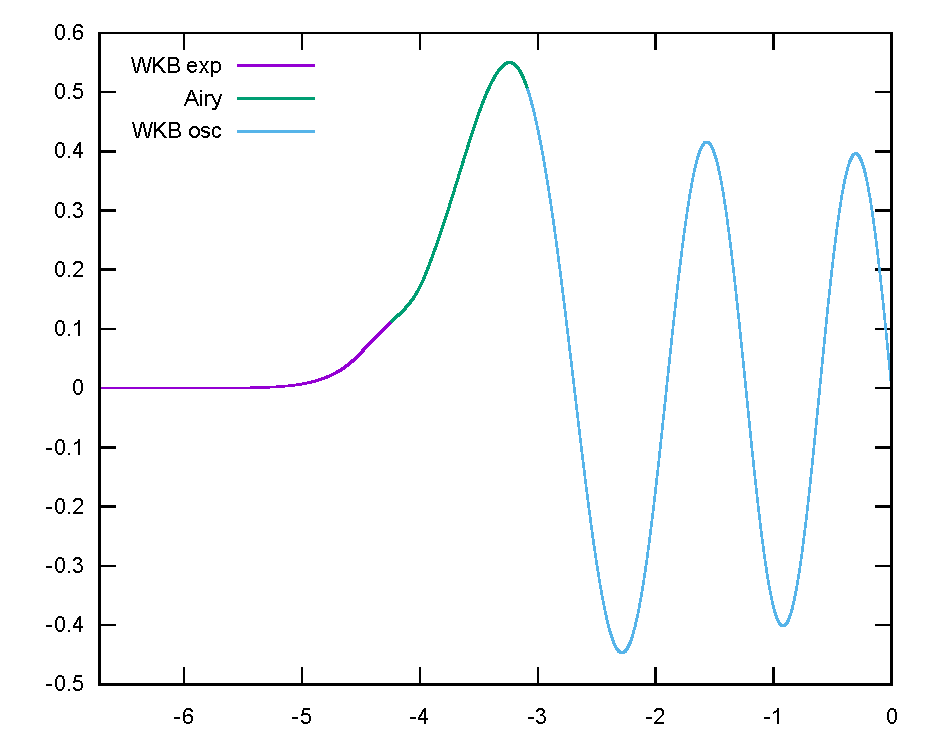
\includegraphics[width=.9\textwidth]{plots/square9half.pdf}
  \caption{Left half of wave function with $N_{Energy} = 9 \Rightarrow E \approx 13.4$, $m = 2$, $V(x) = x^{2}$}\label{fig:wave_parts}
\end{figure}
In figure~\ref{fig:wave_parts} the three parts are visualized. The purple section on the left is the exponentially decaying part $\psi^{WKB}_{exp} (x)$, equation~\ref{eq:wkb:exp} is calculated according to
~\cite[p. 317, Claim 15.7]{hall2013quantum} where $b$ and $a$ are different solutions for $t$ of equation~\ref{eq:wkb:t}. The absolute symbol makes it possible to not
differentiate between the case where $x < t$ and $x > t$.
\subsection{Validity}
When we look at the derivation of WKB we will see that equations \ref{eq:wkb:exp} and \ref{eq:wkb:osc} can only be valid if
\begin{align*}
  p(x) = \sqrt{V(x) - E} \\
  \left|\frac{dp}{dx}(x)\right| \ll p^{2}(x)
\end{align*}
as~\cite{zwiebach2018lecture} showed in his lecture.
But this would mean that WKB is only valid iff $V(x) > E$ because $p^{2}(x)$ would be negative otherwise.
If this is the case this would imply that~\ref{eq:wkb:exp} can't be valid.

We will assume that this contradiction is wrong and assume that WKB is valid if
\[
  \left|\frac{d}{dx}(\sqrt{|V(x) - E|})\right| \ll |V(x) - E|
\]

\subsection{Implementation}
\subsubsection{WKB}
\rustinline{WkbWaveFunction} implements equations~\ref{eq:wkb:exp} and~\ref{eq:wkb:osc}.
The actual equations are implemented in \rustinline{psi_osc} and \rustinline{psi_exp}.
\rustinline{psi_osc} is used if $x$ is inside the classically allowed region otherwise \rustinline{psi_exp} is used.
\begin{rustcode}
fn eval(&self, x: f64) -> Complex64 {
    let val = if self.phase.energy < (self.phase.potential)(x) {
        self.psi_exp(x)
    } else {
        self.psi_osc(x)
    };

    return (self.op)(val);
}
\end{rustcode}
The term \rustinline{self.op} has been an attempt to use both turning points for the oscillating region. It wasn't removed because the
current method is not perfect either and it can be used in the future to improve the accuracy.
\\
For the exponential part the original turning point will still be used. But this means that the exponential will always be positive even if the oscillating part is negative.
To fix this, we can define the \rustinline{get_exp_sign} function.
\begin{rustcode}
pub fn get_exp_sign(&self) -> f64 {
    let limit_sign = if self.turning_point_exp == self.turning_point_osc {
        1.0
    } else {
        -1.0
    };

    (self.psi_osc(self.turning_point_exp + limit_sign * f64::EPSILON.sqrt()) / self.c)
        .re
        .signum()
}
\end{rustcode}
It calculates the sign of the limit of the oscillating region as $x$ approaches the turning point.
\[
  \text{sgn}\left(\lim_{x \to t^{\pm}} \psi^{WKB}_{osc}(x)\right)
\]

\subsubsection{Airy}
The constructor\rustinline{AiryWaveFunction::new} calculates all the turning points in the view and then creates an \rustinline{AiryWaveFunction} for each of them.
These functions are then returned as a pair of the instance and the corresponding turning point.

Just as with the WKB functions, the Airy implementation also implements the \rustinline{self.op} which can be used to implement the osculating region with two turning points


\section{Wave Function Parts}\label{sec:wave-func-parts}
All the equations of the WKB approximation split into multiple parts. This is also reflected in the program architecture.
The trait \rustinline{WaveFunctionPart} represents one of these sections.
\begin{rustcode}
pub trait WaveFunctionPart: Func<f64, Complex64> + Sync + Send {
    fn range(&self) -> (f64, f64);
    fn as_func(&self) -> Box<dyn Func<f64, Complex64>>;
}
\end{rustcode}
These parts all need to implement the \rustinline{Func<_>} trait and are only valid in the range returned by \rustinline{WaveFunctionPart::range}.

As previously mentioned, the architecture has originally been designed around the assumption that both turning points will be used in the oscillating region.
Because of this there is a specialization of this trait that can work with so called ``operations''.
Operations were used to make the transition between the two parts of the osculating regions smoother.
An operation is just a function $f: \mathbb{C} \to \mathbb{C}$ that will be applied over the whole function.
The author decided not to change the architecture to the new method because the program could in theory be extended further.
The wave function parts that support operations implement the \rustinline{WaveFunctionPartWithOp} trait.

\subsection{ApproxPart}
An \rustinline{ApproxPart} is the function around a turning point. This includes the Airy, oscillating WKB and exponential WKB part.
At the same time it also handles the joints between the Airy and WKB functions.

Two joints are constructed and they have the highest ``priority'' when evaluating an ApproxPart for a given $x$.

\begin{rustcode}
fn eval(&self, x: f64) -> Complex64 {
    if is_in_range(self.airy_join_l.range(), x) && ENABLE_AIRY_JOINTS {
        return self.airy_join_l.eval(x);
    } else if is_in_range(self.airy_join_r.range(), x) && ENABLE_AIRY_JOINTS {
        return self.airy_join_r.eval(x);
    } else if is_in_range(self.airy.ts, x) {
        return self.airy.eval(x);
    } else {
        return self.wkb.eval(x);
    }
}
\end{rustcode}
The term ``priority'' is used to say how far up the if statement the function is. Or in other words, functions with a higher priority are preferred. Because the joints overlap with both the ranges of the
Airy and WKB function is important that they are given a higher priority. Further on the range of the Airy part is also included in the WKB range
because of this the WKB part has the least priority.

As we can see, the check if the joints are even enabled happens here, because \rustinline{ENABLE_AIRY_JOINTS} is a constant. The compiler will
remove the branches that are always false automatically (see Appendix~\ref{test:branch-elim}). This means that in theory the program should run a little faster if \rustinline{ENABLE_AIRY_JOINTS} is
disabled. This has to be taken into account when benchmarking.

\subsection{PureWkb}
In the case that there are no turning points or none were found, the program will still try to calculate a wave function. This is done by taking
\rustinline{APPROX_INF} as the turning points. This can be done because no Airy functions will be used. In this case the turning points just act as a bound of
integration.

From experience the results are inaccurate but still usable. At least in the case where the turning points were missed by Newton's method, the WKB parts were fairly accurate, but unsurprisingly diverged at the turning points because there were no Airy functions.

The struct \rustinline{PureWkb} works the same as \rustinline{ApproxPart} but only implements the WKB functions
It does not contain any Airy functions or joints.

\section{Wave Function}
To combine all the \rustinline{WaveFunctionPart} structs, we will define the
\rustinline{WaveFunction} struct. Under the hood it will also calculate all the variables
and construct all the \rustinline{WaveFunctionPart} structs.

First we need to calculate the energy for the given parameters that are passed to the
constructor. Note that this energy will also be printed to the terminal.
\begin{rustcode}
let energy = energy::nth_energy(n_energy, mass, &potential, approx_inf);
println!("{} Energy: {:.9}", Ordinal(n_energy).to_string(), energy);
\end{rustcode}
Using the energy, we can calculate the view as described in section~\ref{sec:view}.
\begin{rustcode}
(
    lower_bound * (upper_bound - lower_bound) * view_factor,
    upper_bound * (upper_bound - lower_bound) * view_factor,
)
\end{rustcode}

Once we've got the view, we can calculate all the turning points and their Airy functions along with them, using \rustinline{AiryWaveFunction::new()}.
In the case that there are turning points we can then go through each turning point and
also copy its neighbors. For the outermost turning points we will take
\rustinline{approx_inf} as its neighbor.

With these groups of 3 we can construct a \rustinline{WkbWaveFunction} for each of the
turning points. However there were issues when dividing the oscillating part of the wave
function was split into two parts with different turning points. As previously mentioned according
to~\cite{hall2013quantum} it should be mathematically indistinguishable when using either of
the turning points, but there arise discontinuities at the transition region. Because of that
it has been decided that only the left turning point will be used.\label{sec:osc_turnging_point_problem}

Unfortunately in this method even though the function is continuous it will not be symmetric
about the midpoint of the oscillating region. This has the effect that the probabilities will
be lower on the right although they should have the same probability.
Because of the architecture of the program, the oscillating part will still be split into two
distinct regions.

While iterating over the turning points we can also calculate the ranges in which the
functions are valid.

Once we have all the \rustinline{WkbWaveFunction} instances we need to group them with the \rustinline{AiryWaveFunction} instances. Using those pairs we can finally construct all the
\rustinline{ApproxPart} instances.

\begin{minipage}{\textwidth}
\noindent Finally we need to apply the \rustinline{scaling} which may be one of the following options (where $a \in \mathbb{C}$):
\begin{description}\label{sec:scaling-type}
    \item[None] The solution won't be multiplied by anything.
    \item[Mul(a)] The solution will be multiplied by $a$.
  \item[Renormalize(a)] $\Psi(x)$ will be renormalized such that
        $
            \int_{-\infty}^{\infty} |a \Psi(x)|^{2} dx = 1
        $. This can be useful to add a phase to the wave function.
\end{description}
\end{minipage}
\\[3ex]
In the case that no turning points are found, WKB will be inaccurate. But for completeness we
will assume that \rustinline{approx_inf} is a turning point. Then two
\rustinline{WkbWaveFunction} instances without the Airy functions can be inserted. This behavior is
implemented in \rustinline{PureWkb}.
Afterwards the same scaling procedure (\ref{sec:scaling-type}) is applied as if there were turning points.

In this case you'll also get a warning in the terminal that no turning points were found,
because the results can be inaccurate.

\subsection{Superposition}
Because the superposition principle is also applicable to energies, it is possible that
$\Psi(x)$ is a sum of wave functions with different energies.

On the implementation side this means that we can create a struct \rustinline{Superposition}
that is constructed with a list of energy levels and \rustinline{ScalingType} that can
be used to construct the previously discussed \rustinline{WaveFunction}.
Its implementation of \rustinline{Func<f64, Complex64>} will then sum over all the results of
the individual \rustinline{WaveFunction} structs.


\chapter{Results}
In this chapter some of the plots calculated by the program are analyzed and discussed.
You can reproduce all the results yourself or calculate according to the manual in the appendix~\ref{sec:manual}.

\section{Wave Functions}
\subsection{Hall Example}\label{sec:resutl:hall}
As a first result let's replicate the example from Hall with the 39th energy of a square potential.
\begin{figure}[H]
  \centering
  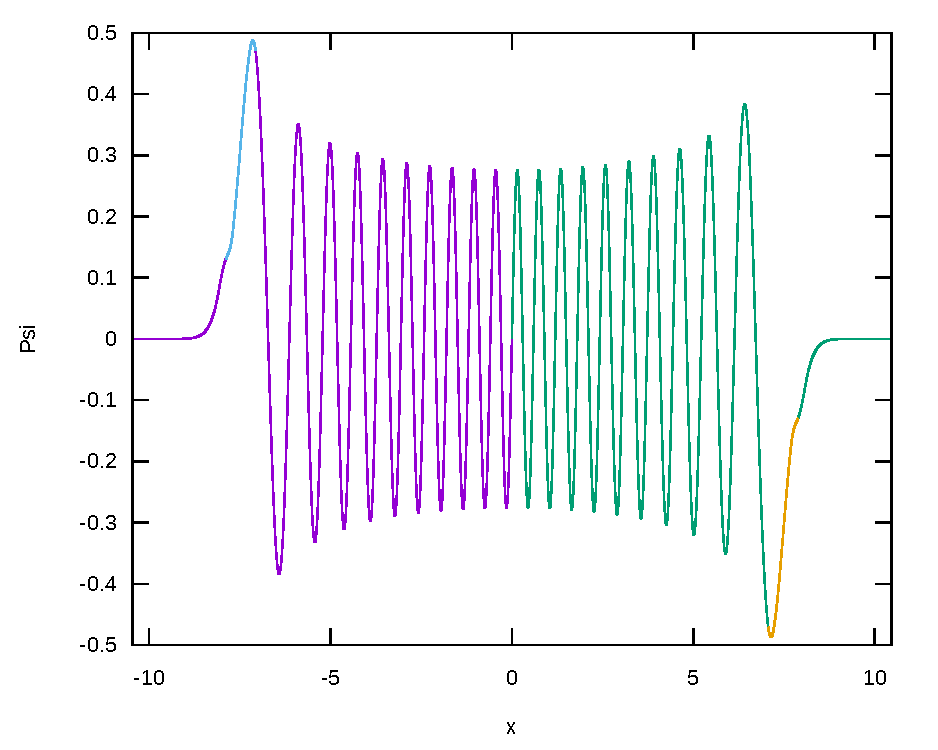
\includegraphics[width=\textwidth]{plots/square-39.pdf}
  \caption{Wave function of 39th energy with $V(x) = x^{2}$, $m = 1$ and $f_{view}=0.1$.}
\end{figure}
This result is very similar to the plot~\cite[fig. 15.5]{hall2013quantum}. The only difference is the joint between the Airy function and the exponential WKB part. In our case the two functions don't
meet as nicely.
Overall the most important thing ought to be the number of maxima and minima which do match.

\subsection{Phase Shift}
Because the Schrödinger equation is linear the wave function can be rotated in the complex plane. For an example we will use a phase of $e^{\mi \frac{\pi}{4}}$ on the wave function of a square potential (figure~\ref{fig:square-12-pi4}).
\begin{figure}[H]
  \centering
  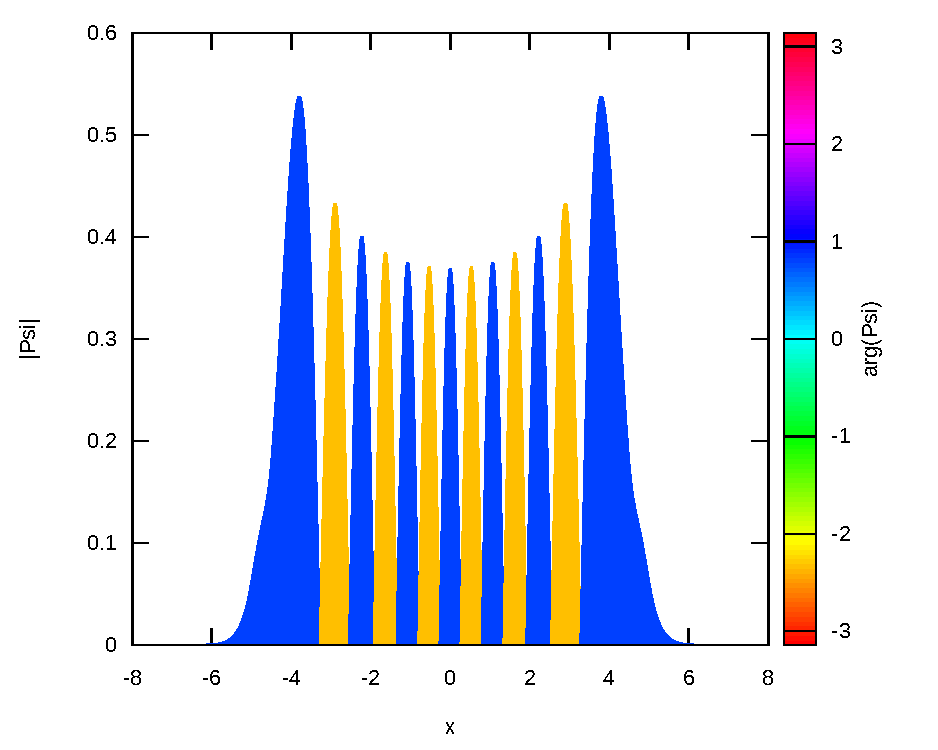
\includegraphics[width=\textwidth]{plots/square-12-pi4.pdf}
  \caption{\label{fig:square-12-pi4} Wave function of 12th energy with $V(x) = x^{2}$, $m = 1$ rotated by $\frac{\pi}{4}$.}
\end{figure}

\subsection{0th Energy}
\begin{minipage}{\textwidth}
In quantum mechanics the 0th energy is not always 0. As an example we will take the 0th
energy of a square potential as shown in figure~\ref{fig:square-0}.
\begin{figure}[H]
  \centering
  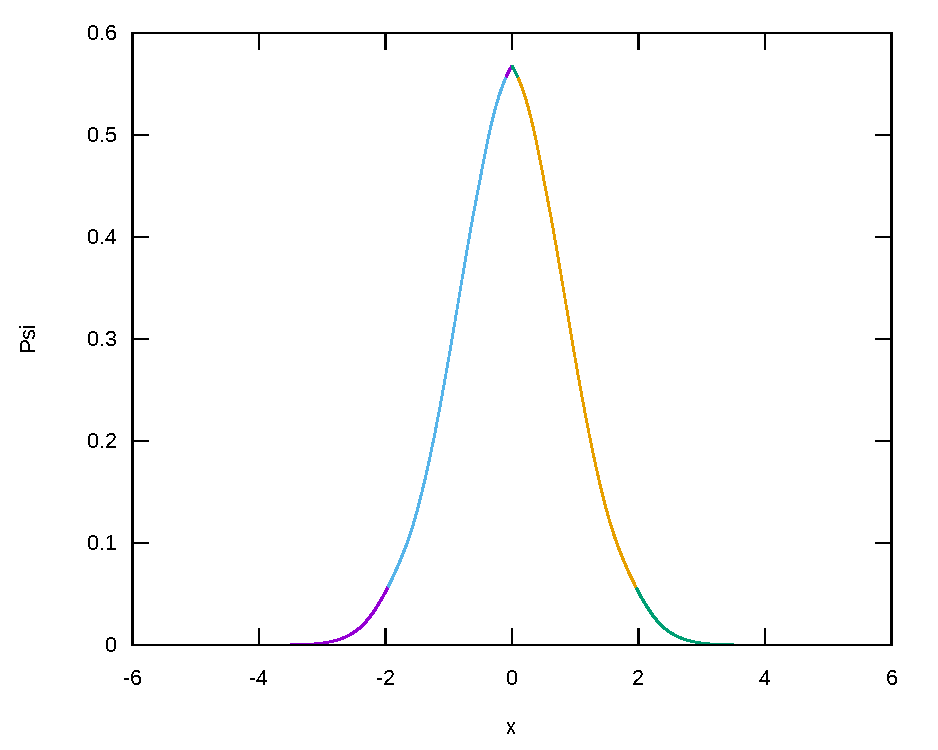
\includegraphics[width=\textwidth]{plots/square-0.pdf}
  \caption{\label{fig:square-0} Wave function of 0th energy with $V(x) = x^{2}$. The function has one maxima and consists almost entirely of Airy functions (blue and yellow). In the middle the function does not seem smooth, see figure~\ref{fig:zoom-square-0} for a closer view.}
\end{figure}
\end{minipage}

\begin{minipage}{\textwidth}
Unfortunately there's a discontinuity at $x = 0$. This shouldn't happen when only using one
turning point and it only seems to be a problem with the 0th energy. This phenomenon has
also been observed for other potentials with the 0th energy.
\begin{figure}[H]
  \centering
  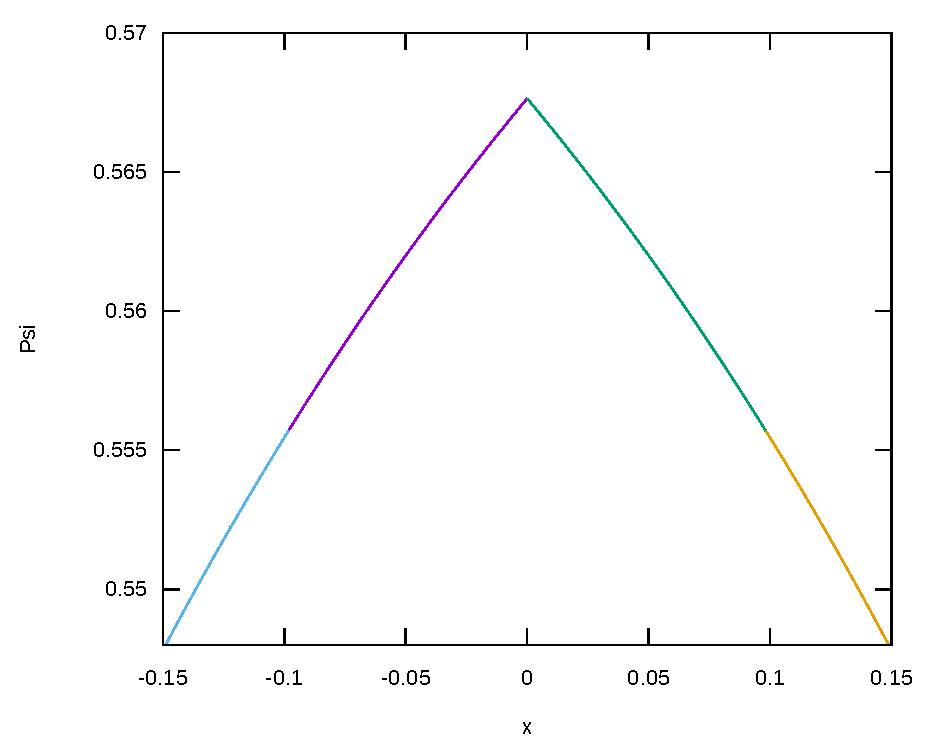
\includegraphics[width=\textwidth]{plots/square-0-zoom.pdf}
  \caption{\label{fig:zoom-square-0} Zoom of wave function of 0th energy with $V(x) = x^{2}$. The two parts meet in the middle and form a unexpected spike. If joints were disabled, the function would be smooth at $x = 0$ but there's also the usual gap between the Airy and WKB functions.}
\end{figure}
\end{minipage}
\vspace*{3ex}

This occurs because the joints of the right and left half overlap to form the ``spike'' in
the middle. Unfortunately this can't be fixed, because one could try to either increase
\rustinline{VALIDITY_LL_FACTOR} to make the two Airy functions overlap which wont be a
perfect fit either. Or it would be possible to decrease \rustinline{AIRY_TRANSITION_FRACTION} which would make the joints smaller, but this would
just make a smooth spike that does not match to the rest of the function.

\begin{minipage}{\textwidth}
As far as the program is concerned $\Psi(x) = 0$ is a valid solution but this has to be done
in a superposition of the same energy with destructive interference.
\[
  \Psi_{super}(x) = 1 \cdot \Psi(x) - 1 \cdot \Psi(x) = 0
\]
In theory this is possible but can't be physically valid because the Schrödinger equation
does not show the full picture. In quantum field theory the wave function would always
oscillate in some way.
\begin{figure}[H]
  \centering
  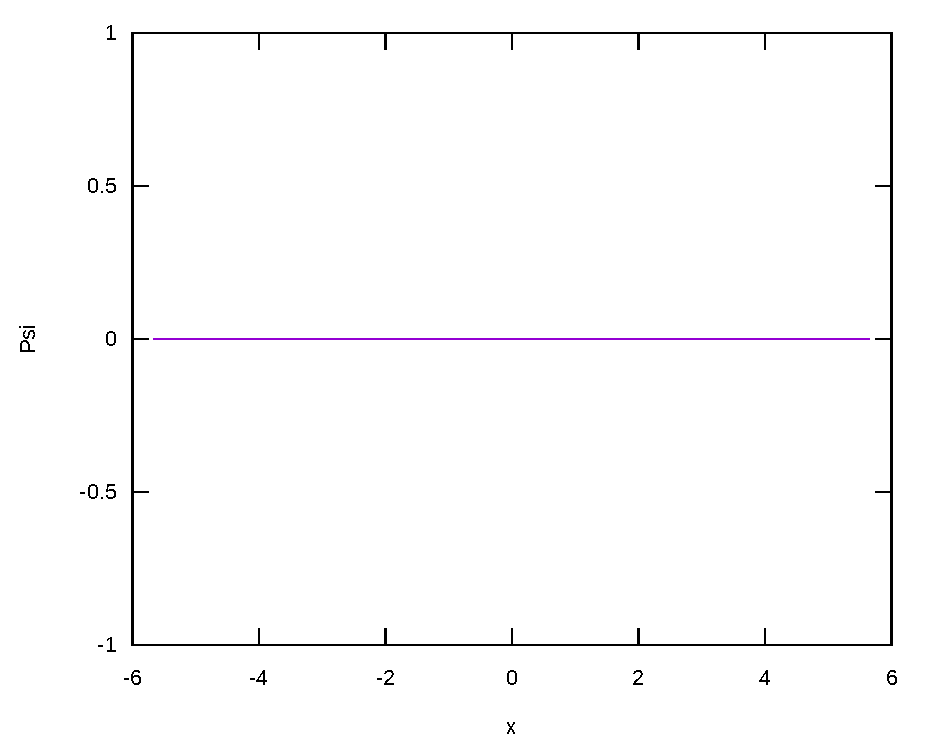
\includegraphics[width=\textwidth]{plots/super-square-0-0-destructive.pdf}
  \caption{Destructive interference of 0th energy with $V(x) = x^{2}$.}
\end{figure}

$\Psi(x) = 0$ would still contain energy; we just can't tell because energy technically only
emerges in the time dependent Schrödinger equation.
\end{minipage}


\section{Mexican Hat Potential}
For this example we will use the ``mexican hat'' potential.
\[
  V(x) = {(x - 4.0)}^{2} {(x + 4.0)}^{2}
\]
It is particularly interesting because it has a maximum. This means that at low energies it will form two oscillations around the two minima.
\begin{figure}[H]
  \centering
  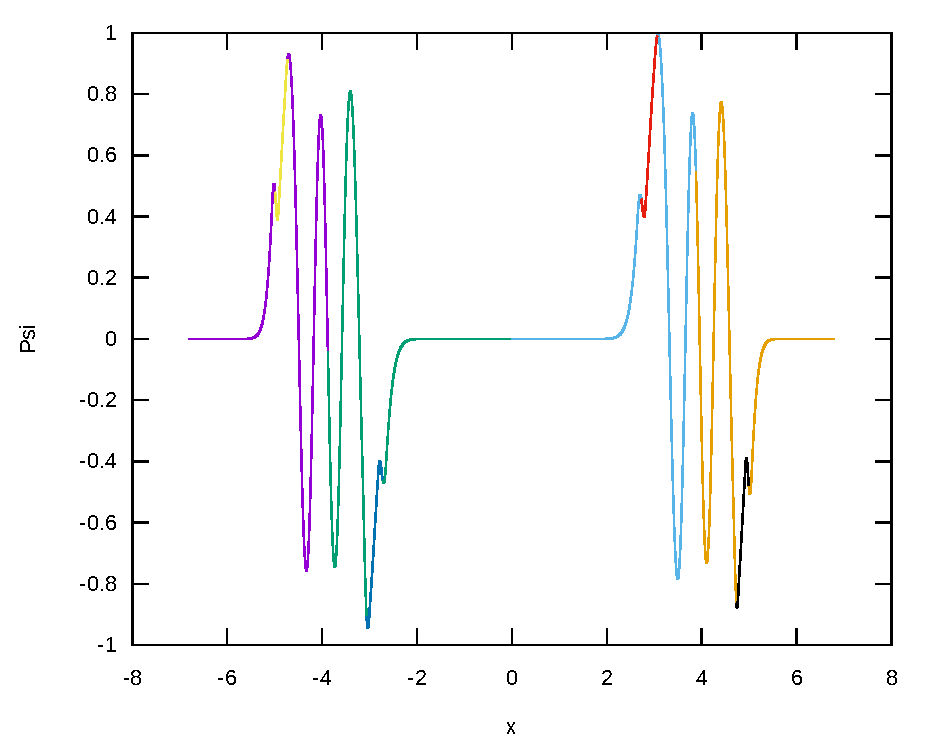
\includegraphics[width=\textwidth]{plots/mexican-hat-10.pdf}
  \caption{Wave function of a mexican hat potential, with nth energy 10 and $m = 1$. The wave function oscillates in two intervals $(-4.85, -2.89)$ and $(2.89, 4.85)$. Between these intervals
    function decease exponentially. The transition region from exponential WKB to Airy appears to have a bigger gap than with a square potential. Even though the two functions should meet at the same
    point, the exponential WKB part seems to have a larger magnitude.}
\end{figure}

\begin{minipage}{\textwidth}
If the energy is high enough, the two oscillations will eventually merge into one as shown in figure~\ref{fig:mexican-hat-56th-energy}.
\begin{figure}[H]
  \centering
  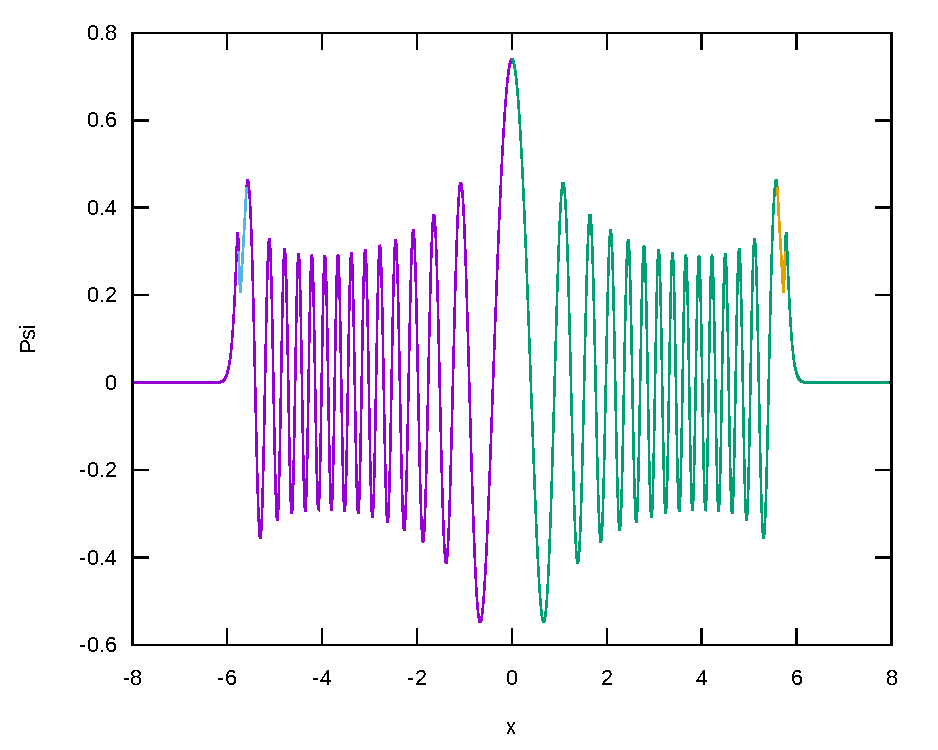
\includegraphics[width=\textwidth]{plots/mexican-hat-56.pdf}
  \caption{
    Wave function of mexican hat potential, with nth energy 56 and $m = 1$. This is the first energy where the oscillating parts combine. The middle of the function has a rather low frequency compared
    to the other oscillating parts.
  }\label{fig:mexican-hat-56th-energy}
\end{figure}
\end{minipage}

\begin{minipage}{\textwidth}
  Unfortunately the program is not able to calculate the 55th energy because Newton's method fails to find the turning points in the middle. And with 54th energy the program doesn't generate any errors
  but the region around $x = 0$ can't be correct (Figure~\ref{fig:mexican-hat-54th-energy}), this occurs because the program fails to detect all the turning points.

\begin{figure}[H]
  \centering
  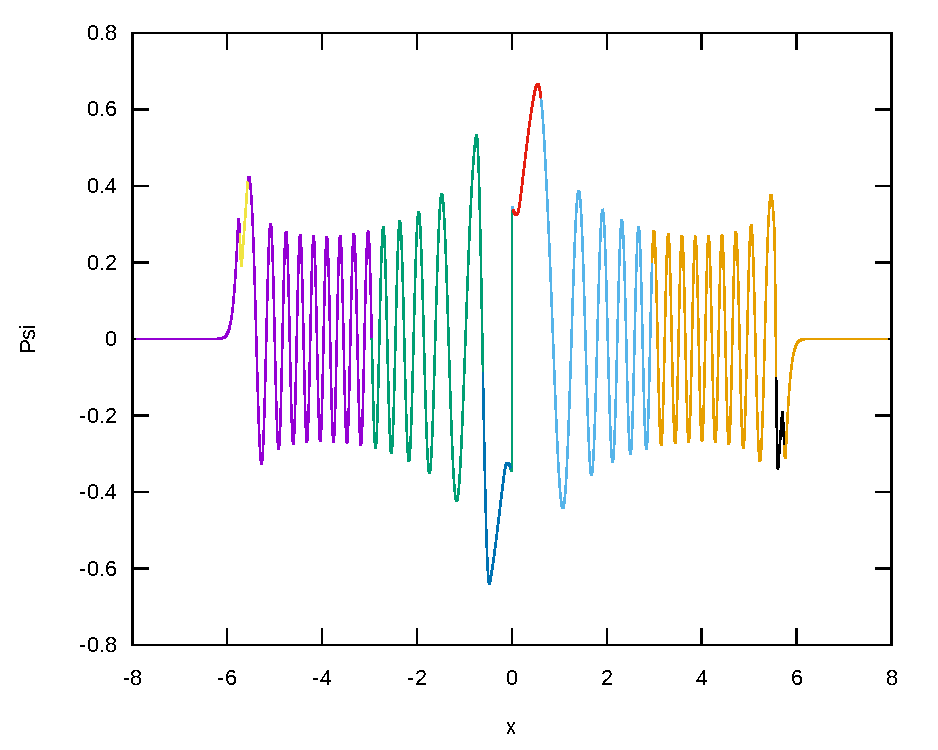
\includegraphics[width=\textwidth]{plots/mexican-hat-53.pdf}
  \caption{
    Wave function of mexican hat potential, with 53rd energy and $m = 1$. Because the oscillating parts are right at the boundary to merge, the wave function has a discontinuity that has been generated by the program at $x = 0$.
  }\label{fig:mexican-hat-53rd-energy}
\end{figure}
But the 53rd energy can be calculated. However there's a discontinuity at $x = 0$ as shown in figure~\ref{fig:mexican-hat-53rd-energy}. This happens because there would be an extra term in the
approximation that handles these cases. When this extension has been implemented, there were problems that most of the wave function would diverge to infinity.
\end{minipage}

\subsection{Superposition}
While some wave functions with superposition of energy seem to be chaotic, others are in some way beautiful because of their symmetries.
Unfortunately the color plots usually don't make the symmetries that arise when plotted in 3D obvious.

\begin{minipage}{\textwidth}
\begin{figure}[H]
\centering
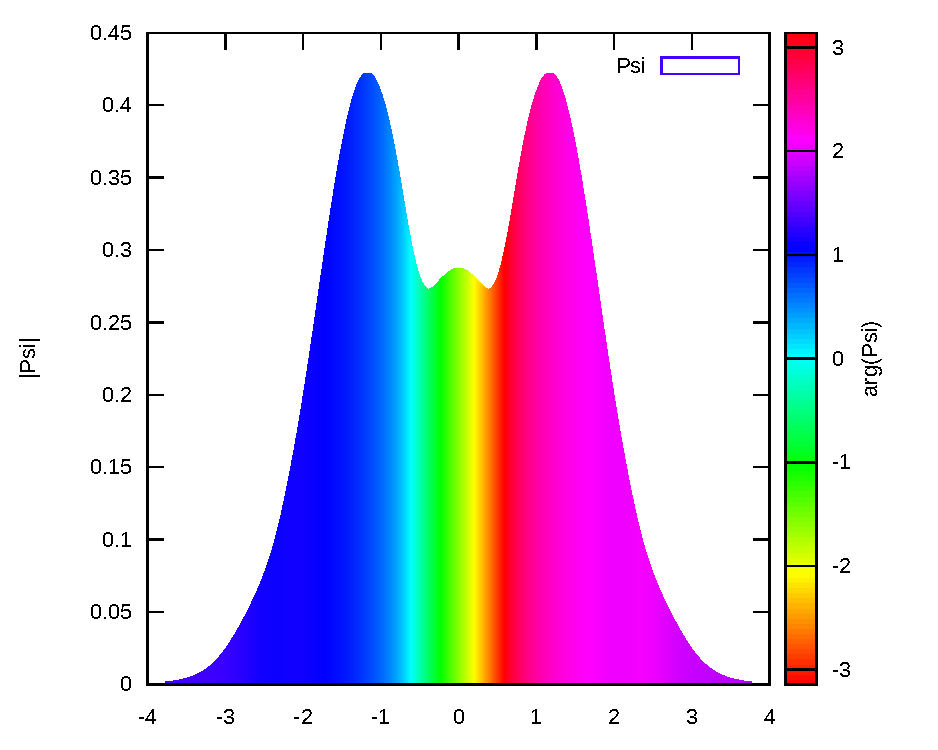
\includegraphics[width=\textwidth]{plots/super-square-1_1-2_i.pdf}
\caption{\label{fig:label} Wave function of square potential, superposition of $1$ times 1st energy and $\mi$ times 2nd energy. The function has three local maxima, it takes a full ``turn'' around
    the complex plane because all the colors only occurs once. Furthermore the two maxima at $x \approx \pm 1.17$ are in opposite directions concerning the angle of the complex plane.}
\end{figure}
This is probably one of the simplest superposition that can be made. In 3D it looks just like a single loop around the x-axis that emerges out of nowhere and disappears again by exponentially decaying.
\end{minipage}

\begin{minipage}{\textwidth}
\begin{figure}[H]
\centering
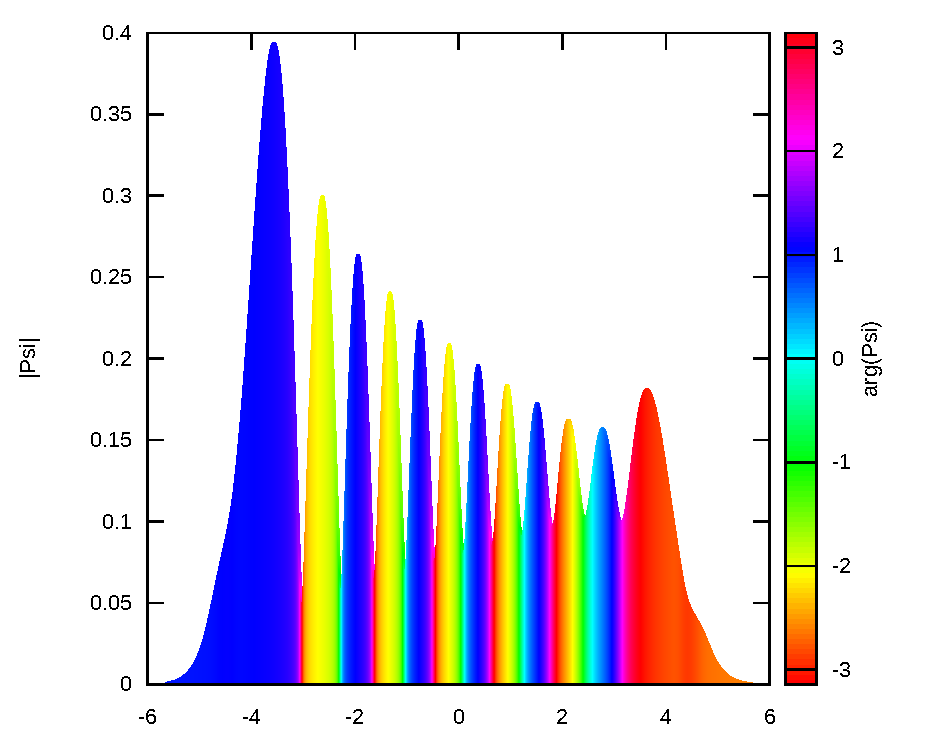
\includegraphics[width=\textwidth]{plots/super-square-10_1-11_1+i.pdf}
\caption{\label{fig:interfence-left}Wave function of square potential, superposition of $1$ times 10th energy and $1+\mi$ times 11th energy. The function has a higher probability towards the left which
  is interesting because both the wave functions for the 10th and 11th energy are symmetrical with respect to the y-axis. Therefore this is an example of quantum interference. The two wave functions
  interact in such a way that the state on the left is far more likely.}
\end{figure}
The same quantum interference as shown in figure~\ref{fig:interfence-left} can be inverted such that a position on the right is more likely by changing the factor of $1+\mi$ to $-1+\mi$ as shown in
figure~\ref{fig:interference-right}.
\end{minipage}

\begin{figure}[H]
\centering
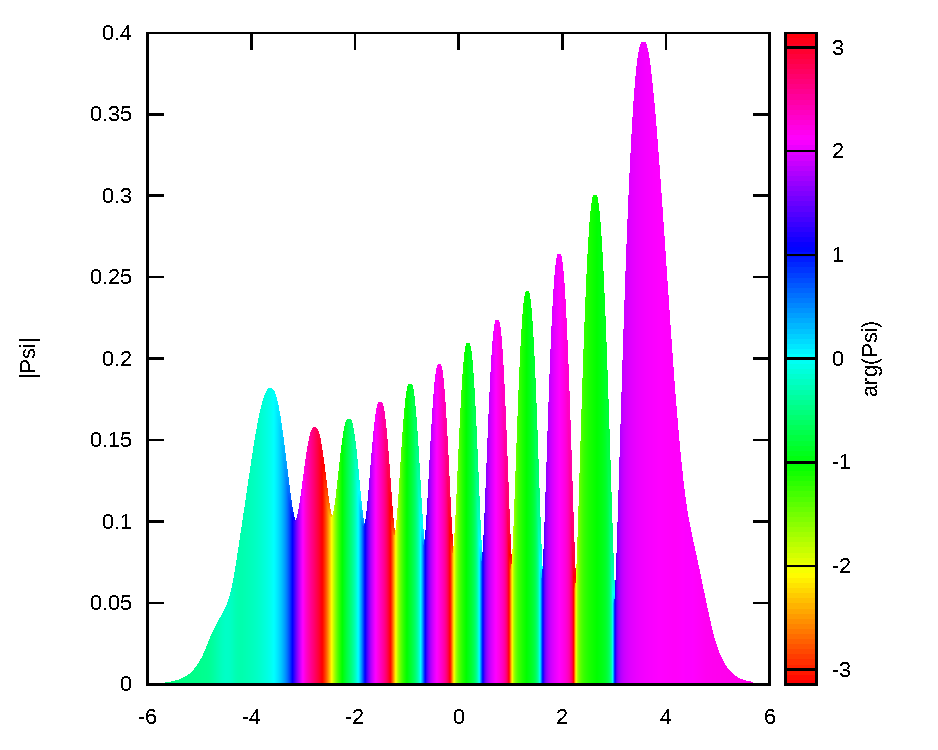
\includegraphics[width=\textwidth]{plots/super-square-10_1-11_-1+i.pdf}
\caption{\label{fig:interference-right} Wave function of square potential, superposition of $1$ times 10th energy and $-1+\mi$ times 11th energy. Just like figure~\ref{fig:interfence-left}
    interference occurs, but in this superposition the probability on the right side of the plot is higher.}
\end{figure}

\section{Performance}
In the appendix there's a detailed description of the test device~\ref{specs:m1}.
\\[3ex]
The overall ``felt performance'' by the user is from the experience of the author quite good. As
expected higher energies generally take longer to run. The same also applies to potentials where simple potentials such as $x^{2}$ are quite fast and complex potentials such as \emph{triple mexican hat}
take longer. Overall the goal that the program should give a quick feed back loop for simple inputs has been achieved because the results were done in under a minute. Particularly the energies 1-6 of
$x^{2}$ can on the test machine be calculated in under 10 s, energies 1-57 in under 30 s and 1-155 in under 1 min. The 155th energy isn't a particularly low energy yet the program still managed to
complete it in under a minute.
\\[3ex]
Apart from the ``percieved'' performance of the user, the benchmarks also show good results. As expected the most time is spent on integration, in particular finding energies and renormalizing the wave
function. Even though energies in an interval of $10$ units are found in almost the same time frame (output~\ref{out:m2:energy-bench}). This is expected due to the algorithm described in
section~\ref{sec:energy-calculation}. These could be fixed by using a greater search area by increasing the variable \rustinline{ENERGY_STEP} in \bashinline{src/energy.rs:47}. The overall evaluation process is fast with 100 samples in 10 ms. One concern
also was that finding turning points would be slow but the measurements indicate that these calculations take less then a millisecond. Even though the bench mark for renormalization is fast, when applied
to actual wave functions, it's really slow because thousands of points have to be calculated.

Performance statistics from perf suggest that the program utilizes the CPU well. The memory layout also seems to be good.
\\[3ex]
All the benchmark results can be found in appendix~\ref{sec:app:benchmarks}.


\section{Accuracy}
To determine the accuracy, the mathematically exact solutions to the Schrödinger equation must be calculated. For simple potentials this can be done with WolframScript.
In the \newline \bashinline{exact.wsl} file exact solutions for the potential $x^{2}$ can be calculated. Note that the energies are still calculated with the Maslov-corrected Bohr–Sommerfeld condition
is used to calculate the energies which is an approximation \citep[p. 307]{hall2013quantum}.
\\[3ex]
When running the script for the 5th energy level, two linearly independent solution \bashinline{psi1} and \bashinline{psi2} are calculated.
\begin{lstlisting}
psi1[x] = ParabolicCylinderD[4.999999999999998, 1.6817928305074292*x]
psi2[x] = ParabolicCylinderD[-5.999999999999998, (0. + 1.6817928305074292*I)*x]
\end{lstlisting}
\bashinline{psi2} will be ignored because it diverges. Afterwards because \bashinline{psi1[x]} is not normalized, it is multiplied such that the maxima of the exact solution match the
maxima of the solutions calculated by \emph{schroedinger\_approx}. In figure~\ref{fig:approx-vs-exact} the two solutions are plotted together.

\begin{figure}[H]
  \centering
  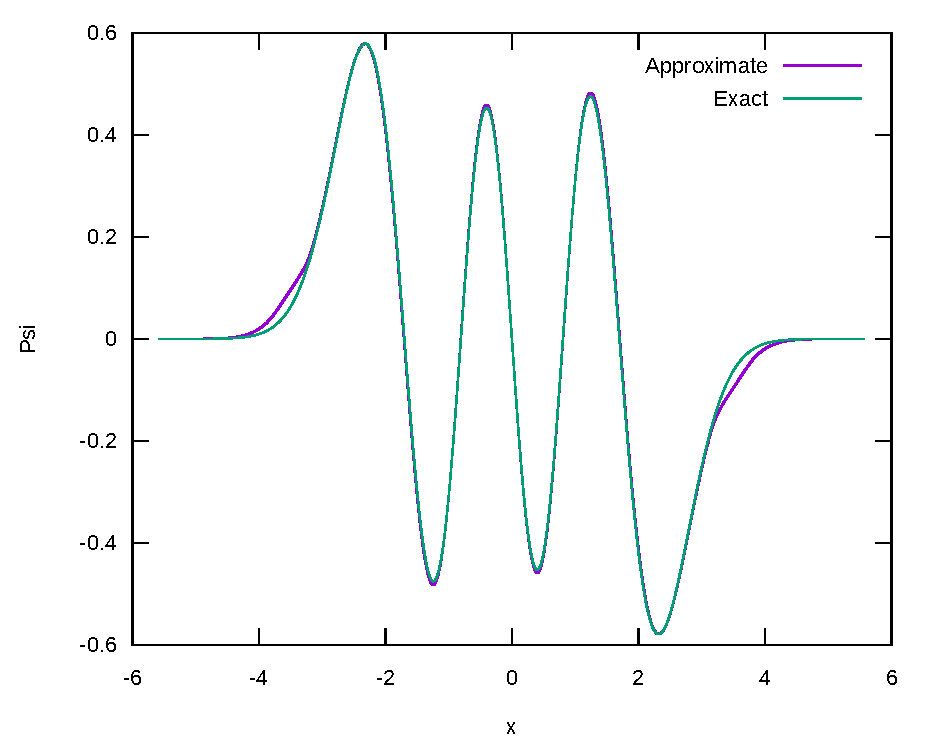
\includegraphics[width=\textwidth]{plots/approx_vs_exact_wave_square_5.pdf}
  \caption{\label{fig:approx-vs-exact} The exact and approximate solution of the 5th energy of the potential $x^{2}$. As expected the greatest error can be seen where the joint between the Airy and
    exponential part was inserted. Otherwise the approximate solution is so close to the real solution that the difference is barely noticeable.}
\end{figure}
The absolute error is plotted in figure~\ref{fig:absolute-error}. Even though the exact solution to the mexican hat potential was not calculated, the error at the transition regions gets worse because
one would expect a smooth exponential decay.
\begin{figure}[H]
  \centering
  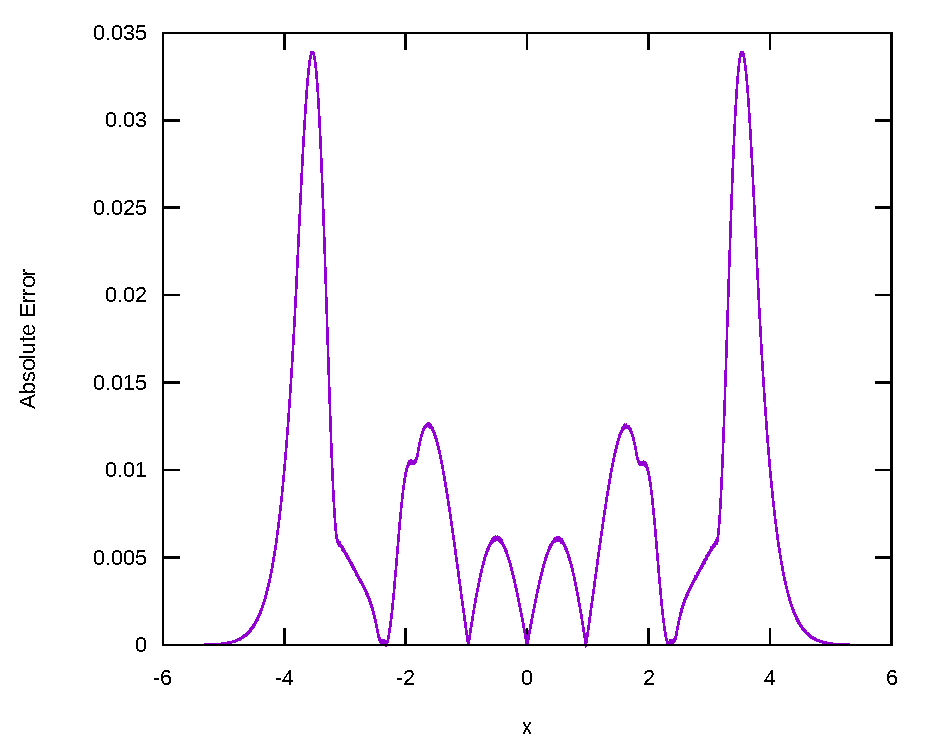
\includegraphics[width=\textwidth]{plots/absolute_error_square_5.pdf}
  \caption{\label{fig:absolute-error} Absolute error of the exact and approximate solution of the 5th energy of the potential $x^{2}$. The error in the semiclassical region is low around 0.01-0.015; this
    meets the goal that the wave function should be ``visually accurate''. At the transition regions the error reaches it's maximum at around 0.034.}
\end{figure}
\begin{figure}[ht]
  \centering
  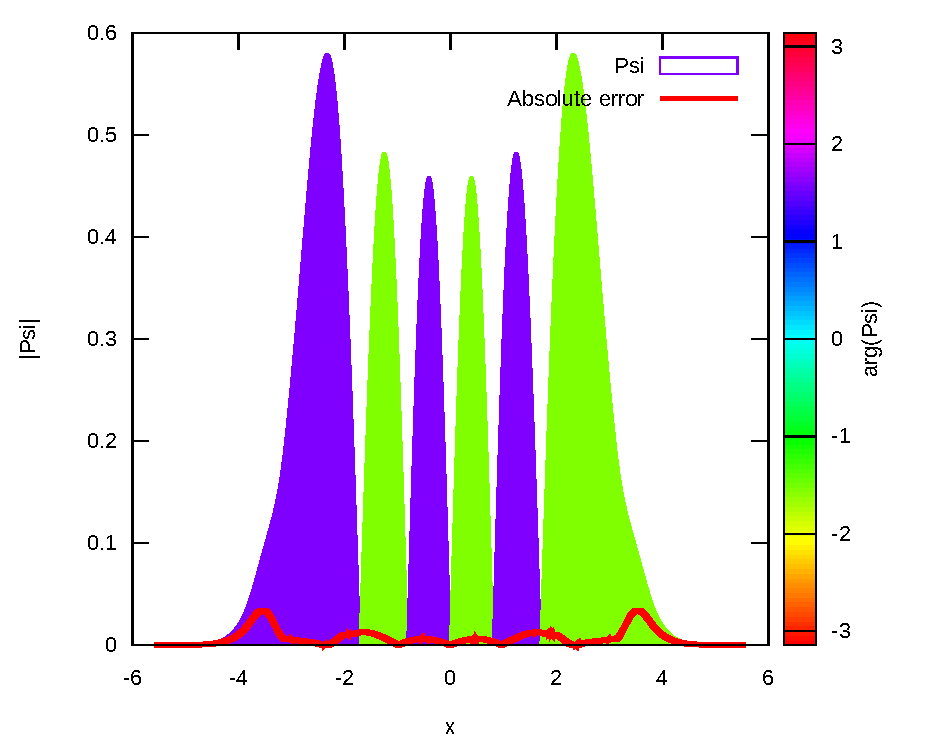
\includegraphics[width=\textwidth]{plots/absolute_error_square_5_with_wave.pdf}
  \caption{\label{fig:absolute-error-with-wave} The absolute error from figure~\ref{fig:absolute-error} is plotted with the approximate wave function. As the violet line indicates, the error reaches a local maximum at the maxima of the wave function itself. }
\end{figure}
The error at the local maxima, as shown in figure~\ref{fig:absolute-error-with-wave}, of the wave function could potentially be lower because the scaling factor of the exact solution is not optimal. This
could be achieved by solving for a minimal area under the curve of the absolute error.

For other energies than 5 the same pattern occurred: the error is greatest at the local maxima of the wave function and even bigger at the transition region.

This error can be minimized by tuning the \rustinline{VALIDITY_LL_FACTOR} constant that makes the Airy functions larger. But this has to be done for each potential separately and the default value of 3.5
should give reasonably good results for most potentials.

\chapter{Conclusion}
In the end the program could be extended and improved almost indefinitely. Unfortunately I had to stop improving it at some point to actually write this paper about how the program works.
Looking back at the goals, the program is quite fast for low and even ``medium'' energies while still being able to calculate solutions for complex potentials. The accuracy can be tuned a little bit
with the constants, but they don't offer a great flexibility.

One of the core design decisions was to follow the UNIX philosophy to some degree and personally I think this has been achieved with the flexible architecture. But as usual the UNIX philosophy has an
impact on the user interface which is probably the weakest part of the program. It is only accessible to programers and can't be used to it's full potential if the user doesn't know Rust, a systems
programing language that is not very similar to popular programing languages like Python. If I have time I will definitely improve the user experience without taking away the freedom to edit the code if
someone would like to.

I might also add a time dependent wave function that uses something simple like Euler's method on the initial WKB solution. In general there are still many things for which there are already utilities
inside the current version of the program. For example, there's an implementation for multidimensional variant of Newton's method that could be used to extend the program to more then one dimension.
\\[3ex]
In the end I gained a deeper understanding of this weird world we're living in and the beauty of the things that can arise from complex mathematics.

\begin{appendix} %Anhang falls nötig
%

\chapter{Program Manual}\label{sec:manual}
\section{Installation of schroedinger\_approx}
This section is a guide on how to install \emph{schroedinger\_approx} on your computer. Please follow the section for your operating system.
\subsection{Linux}
\subsubsection{Ubuntu}
Run the following command to install the dependencies
\begin{bashcode}
sudo apt-get install gnuplot build-essential git libclang-dev
sudo snap go --classic
curl --proto '=https' --tlsv1.2 -sSf https://sh.rustup.rs | sh
source ~/.profile
rustup toolchain add nightly
\end{bashcode}
The curl command that installs Rust will prompt you to choose between installation options, you can choose number \emph{1}.
\\[3ex]
After you've run the script above to install all the dependencies, you can go to the directory where you'd like to install \emph{schroedinger\_approx}. Then run the command
\begin{bashcode}
git clone https://github.com/Gian-Laager/Schroedinger-Approximation.git
\end{bashcode}
to download the code form GitHub.

\subsubsection{Arch Linux}
Run the following command to install all the dependencies
\begin{bashcode}
sudo pacman -Sy gnuplot go git clang
curl --proto '=https' --tlsv1.2 -sSf https://sh.rustup.rs | sh
source ~/.profile
rustup toolchain add nightly
\end{bashcode}
The curl command that installs Rust will prompt you to choose between installation options, you can choose number \emph{1}.
\\[3ex]
After you've run the script above to install all the dependencies, you can go to the directory where you'd like to install \emph{schroedinger\_approx}. Then run the command
\begin{bashcode}
git clone https://github.com/Gian-Laager/Schroedinger-Approximation.git
\end{bashcode}
to download the code form GitHub.

\subsection{macOS}
The following instructions have only been tested under \emph{macOS Ventura 13.0.1} on an Intel CPU. This means the instructions might not work for Apple silicon.
\\[3ex]
First you'll need to install the package manager \emph{Homebrew}, it can be used to install software without downloading all the installers manually. To install it open the \emph{Terminal} program, paste the command below and press enter.
\begin{bashcode}
/bin/bash -c "\$(curl -fsSL https://raw.githubusercontent.com/Homebrew/install/HEAD/install.sh)"
\end{bashcode}

Then you should be asked for your password, type your password (no text will be written while you type your password) and press enter.
Next it will ask you to continue the installation, press enter. This step will take a while because it has to download \emph{Xcode}.
\\[3ex]
After we've installed Homebew, we can install the dependencies of \emph{schroedinger\_approx} with the command
\begin{bashcode}
brew install gnuplot go gcc
\end{bashcode}
\vspace*{3ex}
Next we need to install Rust with the command
\begin{bashcode}
curl --proto '=https' --tlsv1.2 -sSf https://sh.rustup.rs | sh
source ~/.profile
rustup toolchain add nightly
\end{bashcode}
This will ask you to confirm the installation, type \emph{1} and enter.
\\[3ex]
After we've installed all re dependencies you can go to \url{https://github.com/Gian-Laager/Schroedinger-Approximation} and click the green \emph{Code} button,
where you can download the code as a ZIP file.


\subsection{Windows}
Unfortunately \emph{schroedinger\_approx} can't be installed on Windows directly, but since
Windows already supports Linux out of the box in WSL, you can download the latest version of
\emph{Ubuntu} from the Microsoft Store (\url{https://www.microsoft.com/store/productId/9PDXGNCFSCZV}).
\\[3ex]
But first the \emph{WSL optional component} has to be enabled. To do this open the \emph{CMD}
as an administator and run the command
\begin{bashcode}
wsl --install
\end{bashcode}
and reboot once it's finished.
\\[3ex]
After rebooting open \emph{Ubuntu}, this will start the installation automatically. Then
follow the instructions of the terminal. Once your logged in run the commands
\begin{bashcode}
sudo apt-get update
sudo apt-get install build-essential libclang-dev
sudo snap install go --classic
curl --proto '=https' --tlsv1.2 -sSf https://sh.rustup.rs | sh
source ~/.profile
rustup toolchain add nightly
\end{bashcode}
\vspace*{3ex}
To install \emph{gnuplot} open the link
\url{http://gnuplot.info} (you might get a warning that the site is not secure, ignore it and
proceed). There follow the link in the gray box with the title
\emph{Version [\dots] (current)} that says \emph{Release [\dots] ([Date])}. The current
version (\emph{[\dots]}) at the time of writing this document is \emph{5.4.5} but you might
have a newer version available that should also work.
\\[3ex]
After downloading the latest version on \emph{sourceforge} run the installer. In the section
\emph{Select Additional Tasks} set the option \\
\hspace*{3ex}\emph{Add application directory to your PATH environment variable} \\
to true.
\\[3ex]
Now you can download the \emph{schroedinger\_approx} from \url{https://github.com/Gian-Laager/Schroedinger-Approximation}.
Click the green \emph{Code} button and download the code as a ZIP file and extract it to a directory of your choise.
Then you can \emph{drag and drop} the directory to the Ubuntu terminal. This should look something like this
\begin{bashcode}
C:\Users\gianl\OneDrive\Desktop\Schroedinger-Approximation-master
\end{bashcode}
You then need to replace all the \bashinline{\} to \bashinline{/} and change \bashinline{C:} to \bashinline{/mnt/c} (if you have another letter use it's lowercase at \bashinline{/mnt/<your letter>}) and add a \bashinline{cd} at the front. For the example above it would look like this
\begin{bashcode}
cd /mnt/c/Users/gianl/OneDrive/Desktop/Schroedinger-Approximation-master
\end{bashcode}

To run the program, run the command
\begin{bashcode}
cargo run --release
\end{bashcode}

\section{Usage}
In the \bashinline{src} directory you will find the \bashinline{main.rs} file.
After the imports (lines with \rustinline{use}) you can find all the constants that can be
configured. In the description below, (E) stands for ``expert'' and means that you should use the default unless you really know what you're doing.
\begin{description}
    \item[\Large{Concurrency Configurations}] Tune accuracy and performance
        \begin{description}
          \item[\small{INTEG\_STEPS}] The number of steps that will be used to integrate over an interval

          \item[\small{TRAPEZE\_PER\_THREAD (E)}] The number of trapezes that are calculated on a
                thread in sequence. This number must be smaller then
                \rustinline{INTEG_STEPS}.
          \item[\small{NUMBER\_OF\_POINTS}] The number of points that will be written to the output file.

          \item[\small{APPROX\_INF}] This are the values for ``$\pm\infty$''. Where the first number
                is $-\infty$ and the second number is $\infty$. Most importantly outside of
                this interval $V(x) > E$.
        \end{description}

    \item[\Large{Visual Configurations}] Adjust the width of joints
        \begin{description}
          \item[\small{VIEW\_FACTOR}] This factor is used in~\ref{sec:view} as $f_{view}$. It determines in which range the output will be calculated. This depends heavily on the potential and the energy
                and you probably will have to change it. If the wave function is two small and most of the plot is close to $0$ then this factor has to be lowered. If the wave function is not nearly 0 at
                the boundary of the view, this factor should be increased. Note this factor does not influence the calculation itself.

          \item[\small{ENABLE\_WKB\_JOINTS}] If set to \rustinline{true} joints will be added between
                Airy and WKB wave function parts. If set to \rustinline{false} no joints will be added at this boundary.

          \item[\small{AIRY\_TRANSITION\_FRACTION (E)}] When a joint between an Airy and a WKB
                function has to be added, we have to know how wide the joint should be. The
                width is calculated by taking the distance between the turning point
                boundaries and multiplying it by this number.

          \item[\small{VALIDITY\_LL\_FACTOR (E)}] This factor gets used as $a$ in~\ref{eq:valid-airy}. Higher values will create larger ranges for Airy functions.
        \end{description}


\end{description}

\section{WaveFunction}\label{sec:manual:wave-func}
When you only have one energy level you should use \rustinline{WaveFunction::new}.

\begin{rustcode}
    let wave_function = wave_function_builder::WaveFunction::new(
        &/*potential*/,
        /*mass*/,
        /*nth energy*/,
        APPROX_INF,
        1.5,
        ScalingType::/*Scaling*/,
    );
\end{rustcode}
The example above has to be placed right after the \rustinline{fn main()} line.
You have to replace all the commentaries (\rustinline{/*...*/}) with the values you want.
For the first you can choose a potential from section~\ref{sec:potentials} for this you
can type \rustinline{potentials::/*potential*/}.
\\
For the Mass you can just use a normal float.
\\
``nth energy '' must be a positive integer (including 0) and is the nth energy level of the potential.
\\
And as for the scaling type, choose one of the options described at the end of section~\ref{sec:scaling-types}.

\section{Superposition}
To construct a superposition you can add this to your main function
\begin{rustcode}
let wave_function = wave_function_builder::Superposition::new(
    &/*potential*/,
    /*mass*/,
    &[
        (/*nth energy*/, /*phase*/),
        (/*nth energy*/, /*phase*/),
        // ...
    ],
    APPROX_INF,
    1.5, // view factor
    ScalingType::/*scaling*/),
);
\end{rustcode}
Just like in section~\ref{sec:manual:wave-func} you have to replace all the commentaries (\rustinline{/*...*/}) with the values you want.\\
``potential'' you have to choose a potential from section~\ref{sec:potentials}.
\\
``mass'' your mass as a float.
\\
``nth energy '' must be a positive integer (including 0) and is the nth energy level of the potential.
\\
``phase'' a complex number that the wave function with the corresponding energy will be multiplied by. To make a complex number you can use \rustinline{complex(/*Re*/, /*Im*/)}.
\\
``// ...'' you can add as many energies as your computer can handle.
\\
And as for the scaling type, choose one of the options described at the end of section~\ref{sec:scaling-types}.

\section{Plotting}
For all the plotting methods mentioned below you'll need an output directory in which the files will be placed.
\begin{rustcode}
let output_dir = Path::new("output");
\end{rustcode}
The default is \emph{output}, you can choose any directory name that you'd like. The folder will be located where you ran the program.
The data calculated by the program will be stored as space separated values like in the example below (the first line will not be in the output file).
\begin{verbatim}
  x   Re    Im
  1.0 2.718 3.141
  2.0 1.414 1.465
\end{verbatim}
Every line is a data point where the first number is the x-coordinate, the second the real part of $\Psi(x)$ and the third the imaginary part of $\Psi(x)$

\subsection{WaveFunction}
For a \rustinline{WaveFunction} as we've seen in section~\ref{sec:manual:wave-func} you have three options.
\subsubsection{plot\_wavefunction}\label{sec:plot_wavefunction}
With \rustinline{plot::plot_wavefunction} the result will be plotted as one function in gnuplot.
\begin{rustcode}
plot::plot_wavefunction(&wave_function, output_dir, "data.txt");
\end{rustcode}
You can replace \emph{data.txt} with another file name.
\subsubsection{plot\_wavefunction\_parts}
Each pair of $\psi^{WKB}_{osc}$ and $\psi^{WKB}_{exp}$ will be plotted in different colors and the Airy functions will also be plotted separately.

\subsubsection{plot\_probability}\label{sec:plot_probability}
This function will plot the probability $\|\Psi(x)\|^{2}$ of the wave function.

\subsection{Superposition}
\subsubsection{plot\_superposition}
This function plots the superposition analogous to \rustinline{plot_wavefunction} for superpositions.

\subsubsection{plot\_probability\_superposition}
Plots the probability $\|Psi(x)\|^{2}$ of the superposition analogous to~\rustinline{plot_probability}.

\section{Potentials}\label{sec:potentials}
\begin{description}
\begin{minipage}{\textwidth}
  \item[square] Normal square potential as used in~\cite{hall2013quantum}.
        \[
        x^{2}
        \]
        \begin{figure}[H]
          \centering
          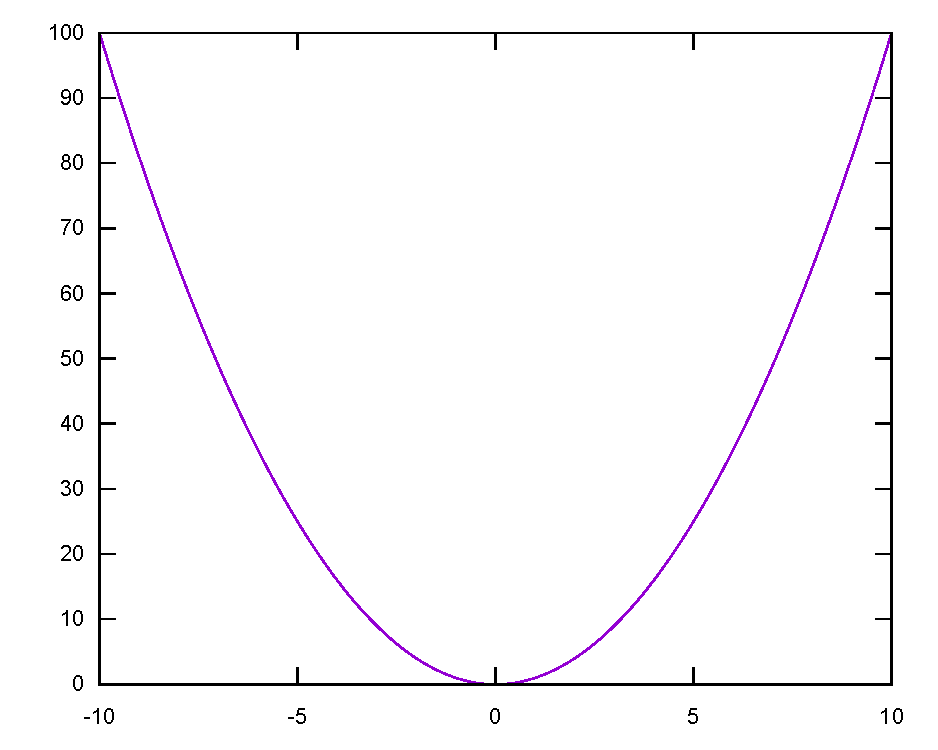
\includegraphics[width=0.65\textwidth]{plots/square.pdf}
        \end{figure}
\end{minipage}
\begin{minipage}{\textwidth}
  \item[mexican\_hat] 4th degree polynomial that looks like a mexican hat, with 2 minima.
        \[
        (x-4)^{2}(x + 4)^{2}
        \]
        \begin{figure}[H]
          \centering
          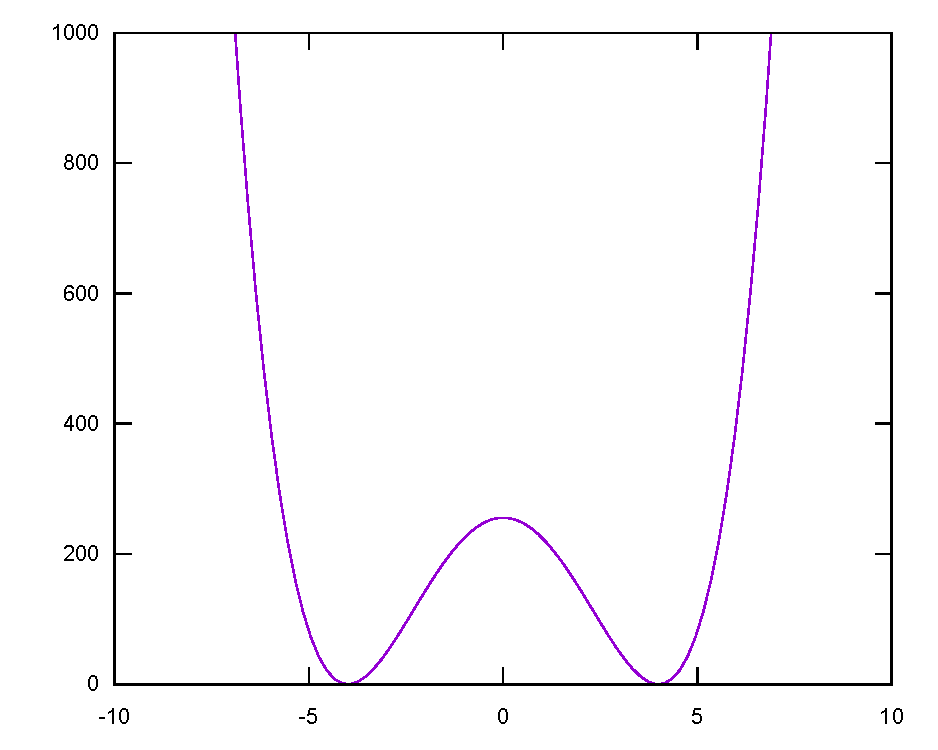
\includegraphics[width=0.65\textwidth]{plots/mexican_hat.pdf}
        \end{figure}
\end{minipage}
\begin{minipage}{\textwidth}
  \item[double\_mexican\_hat] 6th degree polynomial that has 3 minima.
        \[
        (x-4)^{2}x^{2}(x + 4)^{2}
        \]
        \begin{figure}[H]
          \centering
          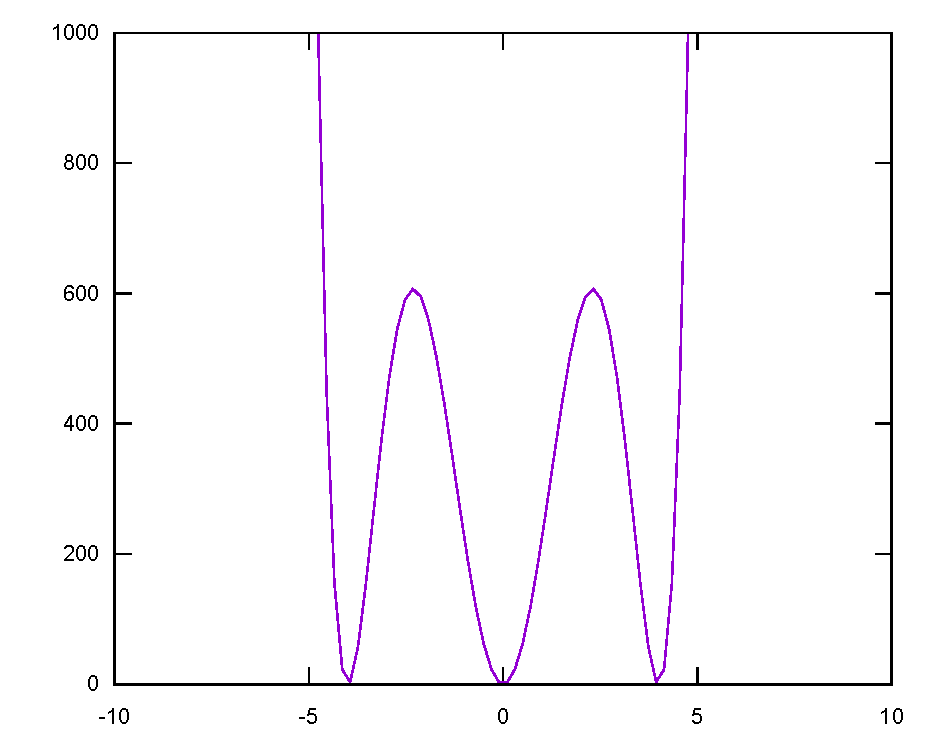
\includegraphics[width=0.65\textwidth]{plots/double_mexican_hat.pdf}
        \end{figure}
\end{minipage}
\begin{minipage}{\textwidth}
  \item[triple\_mexican\_hat] 8th degree polynomial that has 4 minima.
        \[
        (x - 6)^{2}(x - 3)^{2}(x + 3)^{2}(x + 6)^{2}
        \]
        \begin{figure}[H]
          \centering
          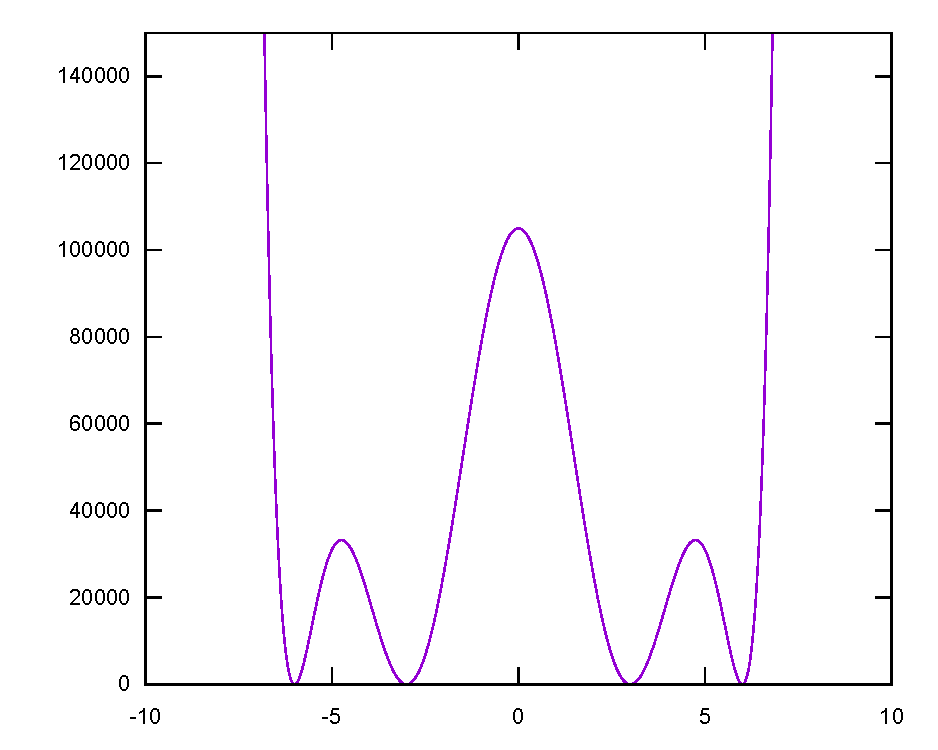
\includegraphics[width=0.65\textwidth]{plots/triple_mexican_hat.pdf}
        \end{figure}
\end{minipage}
  \item[smooth\_step] Step function that goes to \rustinline{ENERGY_INF} outside the interval $(-5, 5)$. Joints were added at $\pm 5$ to make the function differentiable.
\end{description}

\subsection{Custom Potentials}\label{sec:custom-potentials}
To create a custom potential you'll have to define a function like shown below.
\begin{rustcode}
fn my_potential(x: f64) -> f64 {
    return /*some calculation*/;
}
\end{rustcode}
\rustinline{my_potential} is the name that you can choose and have to use later when you're passing it to \rustinline{WaveFunction::new}.
\rustinline{/*some calculation*/} can be any Rust code that results in a \rustinline{f64}.
\\
\subsubsection{Examples}
Negative bell curve ($-e^{-x^{2}} + 1$)
\begin{rustcode}
fn neg_bell(x: f64) -> f64 {
    return -(-x.powi(2)).exp();
}
\end{rustcode}

\noindent General polynomial (might not work for all configurations)
\begin{rustcode}
const COEFFICIENTS: [f64;4] = [a, b, c, d]
fn polynom(x: f64) -> f64 {
    let mut result = 0.0;
    for n in 0..COEFFICIENTS.len() {
        result += x.powi(n) * COEFFICIENTS[n];
    }
    return result;
}
\end{rustcode}
You need to set values for \rustinline{a}, \rustinline{b}, etc. and they need to be floating point numbers or you'll get error E0308. For example \rustinline{1} would cause an error but \rustinline{1.0}
or \rustinline{3.141} are correct. You can add even more coefficients if you'd like. The 4 in the square brackets is the degree of the polynomial plus 1.
The potential above would mathematically be $a + b x + c x^{2} + d x^{3}$.
\chapter{Detailed Calculations and Tests}
\section{Test Machine Specs}
This output was generated by \bashinline{garuda-inxi}. ``[\dots]'' Means the data was removed because it is not necessary.

\subsection{Machine 1}\label{specs:m1}
Machine 1 is the laptop of the author.
\begin{verbatim}
System:
  Kernel: 6.0.9-zen1-1-zen arch: x86_64 bits: 64 compiler: gcc v: 12.2.0
    parameters: BOOT_IMAGE=/@/boot/vmlinuz-linux-zen
    root=UUID=308b5626-2597-4f46-9f16-a4d882bf2bf0 rw rootflags=subvol=@
    quiet splash rd.udev.log_priority=3 vt.global_cursor_default=0
    systemd.unified_cgroup_hierarchy=1 loglevel=3 ibt=off
  Console: pty pts/0 DM: SDDM Distro: Garuda Linux base: Arch Linux
Machine:
  Type: Laptop System: ASUSTeK product: ROG Zephyrus G14 GA401QM_GA401QM
    v: 1.0 serial: <filter>
  Mobo: ASUSTeK model: GA401QM v: 1.0 serial: <filter> UEFI: American
    Megatrends LLC. v: GA401QM.412 date: 08/30/2022

[...]

CPU:
  Info: model: AMD Ryzen 9 5900HS with Radeon Graphics socket: FP6 bits: 64
    type: MT MCP arch: Zen 3 gen: 4 level: v3 note: check built: 2021-22
    process: TSMC n7 (7nm) family: 0x19 (25) model-id: 0x50 (80) stepping: 0
    microcode: 0xA50000C
  Topology: cpus: 1x cores: 8 tpc: 2 threads: 16 smt: enabled cache:
    L1: 512 KiB desc: d-8x32 KiB; i-8x32 KiB L2: 4 MiB desc: 8x512 KiB
    L3: 16 MiB desc: 1x16 MiB
  Speed (MHz): avg: 3300 min/max: 1200/4679 boost: enabled
    base/boost: 3300/4650 scaling: driver: acpi-cpufreq governor: performance
    volts: 1.2 V ext-clock: 100 MHz cores: 1: 3300 2: 3300 3: 3300 4: 3300
    5: 3300 6: 3300 7: 3300 8: 3300 9: 3300 10: 3300 11: 3300 12: 3300
    13: 3300 14: 3300 15: 3300 16: 3300 bogomips: 105400
  Flags: avx avx2 ht lm nx pae sse sse2 sse3 sse4_1 sse4_2 sse4a ssse3 svm
  Vulnerabilities:
  Type: itlb_multihit status: Not affected
  Type: l1tf status: Not affected
  Type: mds status: Not affected
  Type: meltdown status: Not affected
  Type: mmio_stale_data status: Not affected
  Type: retbleed status: Not affected
  Type: spec_store_bypass mitigation: Speculative Store Bypass disabled via
    prctl
  Type: spectre_v1 mitigation: usercopy/swapgs barriers and __user pointer
    sanitization
  Type: spectre_v2 mitigation: Retpolines, IBPB: conditional, IBRS_FW,
    STIBP: always-on, RSB filling, PBRSB-eIBRS: Not affected
  Type: srbds status: Not affected
  Type: tsx_async_abort status: Not affected

[...]

Garuda (2.6.9-1):
  System install date:     2022-01-06
  Last full system update: 2022-11-19
  Is partially upgraded:   No
  Relevant software:       NetworkManager
  Windows dual boot:       Yes
  Snapshots:               Snapper
  Failed units:            shadow.service snapper-cleanup.service
\end{verbatim}

\subsection{Machine 2}\label{specs:m2}
Machine 2 is a VM running Ubuntu 20.04.1 LTS on the server of Fridolins Robotik (FRC team 6417).
\begin{verbatim}
System:
  Kernel: 5.4.0-132-generic x86_64 bits: 64 compiler: gcc v: 9.4.0
  parameters: BOOT_IMAGE=/vmlinuz-5.4.0-132-generic
  root=/dev/mapper/ubuntu--vg-ubuntu--lv ro maybe-ubiquity
  Console: tty 0 dm: N/A Distro: Ubuntu 20.04.1 LTS (Focal Fossa)
Machine:
  Type: Kvm System: QEMU product: Standard PC (i440FX + PIIX, 1996)
  v: pc-i440fx-6.1 serial: <filter> Chassis: type: 1 v: pc-i440fx-6.1
  serial: <filter>
  Mobo: N/A model: N/A serial: N/A BIOS: SeaBIOS
  v: rel-1.14.0-0-g155821a1990b-prebuilt.qemu.org date: 04/01/2014
CPU:
  Topology: 24-Core model: Common KVM bits: 64 type: MCP arch: K8
  family: F (15) model-id: 6 stepping: 1 microcode: 1000065
  L2 cache: 12.0 MiB
  flags: lm nx pae sse sse2 sse3 bogomips: 138938
  Speed: 2895 MHz min/max: N/A Core speeds (MHz): 1: 2895 2: 2895 3: 2895
  4: 2895 5: 2895 6: 2895 7: 2895 8: 2895 9: 2895 10: 2895 11: 2895 12: 2895
  13: 2895 14: 2895 15: 2895 16: 2895 17: 2895 18: 2895 19: 2895 20: 2895
  21: 2895 22: 2895 23: 2895 24: 2895
  Vulnerabilities: Type: itlb_multihit status: Not affected
  Type: l1tf status: Not affected
  Type: mds status: Not affected
  Type: meltdown status: Not affected
  Type: mmio_stale_data status: Not affected
  Type: retbleed status: Not affected
  Type: spec_store_bypass status: Not affected
  Type: spectre_v1
  mitigation: usercopy/swapgs barriers and __user pointer sanitization
  Type: spectre_v2 mitigation: Retpolines, STIBP: disabled, RSB filling,
  PBRSB-eIBRS: Not affected
  Type: srbds status: Not affected
  Type: tsx_async_abort status: Not affected

[...]

Info:
  Processes: 288 Uptime: 1m Memory: 3.83 GiB used: 345.0 MiB (8.8%)
  Init: systemd v: 245 runlevel: 5 Compilers: gcc: 9.4.0 alt: 9
  Shell: garuda-inxi running in: tty 0 (SSH) inxi: 3.0.38
\end{verbatim}

\section{Benchmarks}\label{sec:app:benchmarks}
\subsection{Rust Benchmarks}
\renewcommand{\lstlistingname}{Output} % Listing->Code
These benchmarks were performed after a reboot of test machine 1 (specs~\ref{specs:m1}) in a TTY to minimize the CPU usage of other processes.
\begin{lstlisting}[caption={
Test run on machine 1, the energy tests were ignored because they take about 2 hours to run.
}]
test benchmarks::test::energy_bench_nenergy_1             ... ignored
test benchmarks::test::energy_bench_nenergy_2             ... ignored
test benchmarks::test::energy_bench_nenergy_3             ... ignored
test benchmarks::test::energy_bench_nenergy_4             ... ignored
test benchmarks::test::energy_bench_nenergy_5             ... ignored
test benchmarks::test::energy_bench_nenergy_6             ... ignored
test benchmarks::test::energy_bench_nenergy_7             ... ignored
test benchmarks::test::energy_bench_nenergy_8             ... ignored
test benchmarks::test::energy_bench_nenergy_9             ... ignored
test benchmarks::test::evaluate_bench_nenergy_1           ... bench:  11,106,464 ns/iter (+/- 1,746,488)
test benchmarks::test::evaluate_bench_nenergy_2           ... bench:  10,952,637 ns/iter (+/- 3,015,099)
test benchmarks::test::evaluate_bench_nenergy_3           ... bench:  10,779,924 ns/iter (+/- 1,115,300)
test benchmarks::test::evaluate_bench_nenergy_4           ... bench:  10,674,015 ns/iter (+/- 1,218,173)
test benchmarks::test::evaluate_bench_nenergy_5           ... bench:  10,597,315 ns/iter (+/- 1,565,714)
test benchmarks::test::evaluate_bench_nenergy_6           ... bench:  10,394,542 ns/iter (+/- 1,370,995)
test benchmarks::test::evaluate_bench_nenergy_7           ... bench:  10,459,327 ns/iter (+/- 3,031,317)
test benchmarks::test::evaluate_bench_nenergy_8           ... bench:  10,426,418 ns/iter (+/- 1,183,630)
test benchmarks::test::evaluate_bench_nenergy_9           ... bench:  10,168,316 ns/iter (+/- 1,286,419)
test turning_points::test::turning_point_square_nenergy_1 ... bench:     352,416 ns/iter (+/- 14,520)
test turning_points::test::turning_point_square_nenergy_2 ... bench:     345,360 ns/iter (+/- 18,186)
test turning_points::test::turning_point_square_nenergy_3 ... bench:     334,762 ns/iter (+/- 10,151)
test turning_points::test::turning_point_square_nenergy_4 ... bench:     320,085 ns/iter (+/- 17,957)
test turning_points::test::turning_point_square_nenergy_5 ... bench:     337,889 ns/iter (+/- 16,637)
test turning_points::test::turning_point_square_nenergy_6 ... bench:     319,445 ns/iter (+/- 140,482)
test turning_points::test::turning_point_square_nenergy_7 ... bench:     318,446 ns/iter (+/- 19,353)
test turning_points::test::turning_point_square_nenergy_8 ... bench:     321,418 ns/iter (+/- 135,708)
test turning_points::test::turning_point_square_nenergy_9 ... bench:     325,621 ns/iter (+/- 18,741)
test wave_function_builder::test::renormalize_square      ... bench:     147,407 ns/iter (+/- 11,088)
\end{lstlisting}
\vspace*{3ex}
\begin{lstlisting}[caption={
Test on machine 2 (specs~\ref{specs:m2}).
}]
test benchmarks::test::energy_bench_nenergy_1             ... ignored
test benchmarks::test::energy_bench_nenergy_2             ... ignored
test benchmarks::test::energy_bench_nenergy_3             ... ignored
test benchmarks::test::energy_bench_nenergy_4             ... ignored
test benchmarks::test::energy_bench_nenergy_5             ... ignored
test benchmarks::test::energy_bench_nenergy_6             ... ignored
test benchmarks::test::energy_bench_nenergy_7             ... ignored
test benchmarks::test::energy_bench_nenergy_8             ... ignored
test benchmarks::test::energy_bench_nenergy_9             ... ignored
test benchmarks::test::evaluate_bench_nenergy_1           ... bench:  25,078,868 ns/iter (+/- 7,078,947)
test benchmarks::test::evaluate_bench_nenergy_2           ... bench:  24,153,512 ns/iter (+/- 5,987,513)
test benchmarks::test::evaluate_bench_nenergy_3           ... bench:  24,043,451 ns/iter (+/- 6,440,041)
test benchmarks::test::evaluate_bench_nenergy_4           ... bench:  23,665,692 ns/iter (+/- 6,265,762)
test benchmarks::test::evaluate_bench_nenergy_5           ... bench:  22,671,743 ns/iter (+/- 5,090,286)
test benchmarks::test::evaluate_bench_nenergy_6           ... bench:  23,273,191 ns/iter (+/- 6,871,818)
test benchmarks::test::evaluate_bench_nenergy_7           ... bench:  23,143,284 ns/iter (+/- 6,225,635)
test benchmarks::test::evaluate_bench_nenergy_8           ... bench:  23,470,605 ns/iter (+/- 6,941,491)
test benchmarks::test::evaluate_bench_nenergy_9           ... bench:  22,564,435 ns/iter (+/- 5,548,813)
test turning_points::test::turning_point_square_nenergy_1 ... bench:   1,871,010 ns/iter (+/- 826,263)
test turning_points::test::turning_point_square_nenergy_2 ... bench:   1,928,734 ns/iter (+/- 893,799)
test turning_points::test::turning_point_square_nenergy_3 ... bench:   1,750,410 ns/iter (+/- 972,254)
test turning_points::test::turning_point_square_nenergy_4 ... bench:   1,826,680 ns/iter (+/- 986,256)
test turning_points::test::turning_point_square_nenergy_5 ... bench:   1,943,480 ns/iter (+/- 1,000,387)
test turning_points::test::turning_point_square_nenergy_6 ... bench:   1,887,249 ns/iter (+/- 806,322)
test turning_points::test::turning_point_square_nenergy_7 ... bench:   1,781,980 ns/iter (+/- 846,578)
test turning_points::test::turning_point_square_nenergy_8 ... bench:   1,957,382 ns/iter (+/- 908,014)
test turning_points::test::turning_point_square_nenergy_9 ... bench:   1,919,896 ns/iter (+/- 962,210)
test wave_function_builder::test::renormalize_square      ... bench:     813,134 ns/iter (+/- 675,427)

\end{lstlisting}

\begin{lstlisting}[caption={
Previously ignored energy tests on machine 2
}, label=out:m2:energy-bench]
running 9 tests
test benchmarks::test::energy_bench_nenergy_1             ... bench: 2,066,938,596 ns/iter (+/- 122,637,612)
test benchmarks::test::energy_bench_nenergy_2             ... bench: 2,087,782,039 ns/iter (+/- 135,082,403)
test benchmarks::test::energy_bench_nenergy_3             ... bench: 2,093,995,693 ns/iter (+/- 156,802,393)
test benchmarks::test::energy_bench_nenergy_4             ... bench: 2,069,512,511 ns/iter (+/- 102,294,553)
test benchmarks::test::energy_bench_nenergy_5             ... bench: 2,079,575,086 ns/iter (+/- 129,997,432)
test benchmarks::test::energy_bench_nenergy_6             ... bench: 2,091,588,104 ns/iter (+/- 134,889,997)
test benchmarks::test::energy_bench_nenergy_7             ... bench: 4,149,571,071 ns/iter (+/- 225,497,112)
test benchmarks::test::energy_bench_nenergy_8             ... bench: 4,175,954,724 ns/iter (+/- 201,706,134)
test benchmarks::test::energy_bench_nenergy_9             ... bench: 4,175,015,897 ns/iter (+/- 163,725,865)

test result: ok. 0 passed; 0 failed; 0 ignored; 9 measured; 35 filtered out; finished in 7521.30s
\end{lstlisting}
\renewcommand{\lstlistingname}{Code Snippet} % Listing->Code

\subsection{Perf}
\bashinline{perf stat -d -d -d -repeat 100} on superposition of energies 1 through 9 of $x^{2}$.
\begin{lstlisting}
# started on Sat Nov 19 22:21:53 2022


 Performance counter stats for './target/release/schroedinger_approx' (100 runs):

      2,446,386.86 msec task-clock                       #   15.938 CPUs utilized            ( +-  0.07% )
           769,294      context-switches                 #  314.455 /sec                     ( +-  0.73% )
            18,443      cpu-migrations                   #    7.539 /sec                     ( +-  0.92% )
            44,453      page-faults                      #   18.171 /sec                     ( +-  1.21% )
 7,820,854,372,190      cycles                           #    3.197 GHz                      ( +-  0.05% )  (40.00%)
     8,485,422,199      stalled-cycles-frontend          #    0.11% frontend cycles idle     ( +- 28.66% )  (40.00%)
     9,501,600,446      stalled-cycles-backend           #    0.12% backend cycles idle      ( +-  1.14% )  (40.00%)
14,477,558,852,335      instructions                     #    1.85  insn per cycle
                                                  #    0.00  stalled cycles per insn  ( +-  0.01% )  (40.00%)
 1,384,019,071,011      branches                         #  565.729 M/sec                    ( +-  0.02% )  (40.00%)
       818,139,391      branch-misses                    #    0.06% of all branches          ( +-  0.45% )  (40.00%)
 5,582,382,628,800      L1-dcache-loads                  #    2.282 G/sec                    ( +-  0.02% )  (40.00%)
   115,562,637,690      L1-dcache-load-misses            #    2.07% of all L1-dcache accesses  ( +-  0.17% )  (40.00%)
   <not supported>      LLC-loads
   <not supported>      LLC-load-misses
    12,523,189,958      L1-icache-loads                  #    5.119 M/sec                    ( +-  0.48% )  (40.00%)
        80,902,476      L1-icache-load-misses            #    0.64% of all L1-icache accesses  ( +-  0.61% )  (40.00%)
     2,380,836,711      dTLB-loads                       #  973.186 K/sec                    ( +-  1.10% )  (40.00%)
        53,829,893      dTLB-load-misses                 #    2.37% of all dTLB cache accesses  ( +-  1.68% )  (40.00%)
        34,803,159      iTLB-loads                       #   14.226 K/sec                    ( +-  2.36% )  (40.00%)
        17,518,263      iTLB-load-misses                 #   39.70% of all iTLB cache accesses  ( +-  1.86% )  (40.00%)
   106,080,681,746      L1-dcache-prefetches             #   43.361 M/sec                    ( +-  0.00% )  (40.00%)
   <not supported>      L1-dcache-prefetch-misses

           153.498 +- 0.128 seconds time elapsed  ( +-  0.08% )
\end{lstlisting}

\section{Additional Plots}
\subsection{Mexican Hat}
\begin{figure}[H]
  \centering
    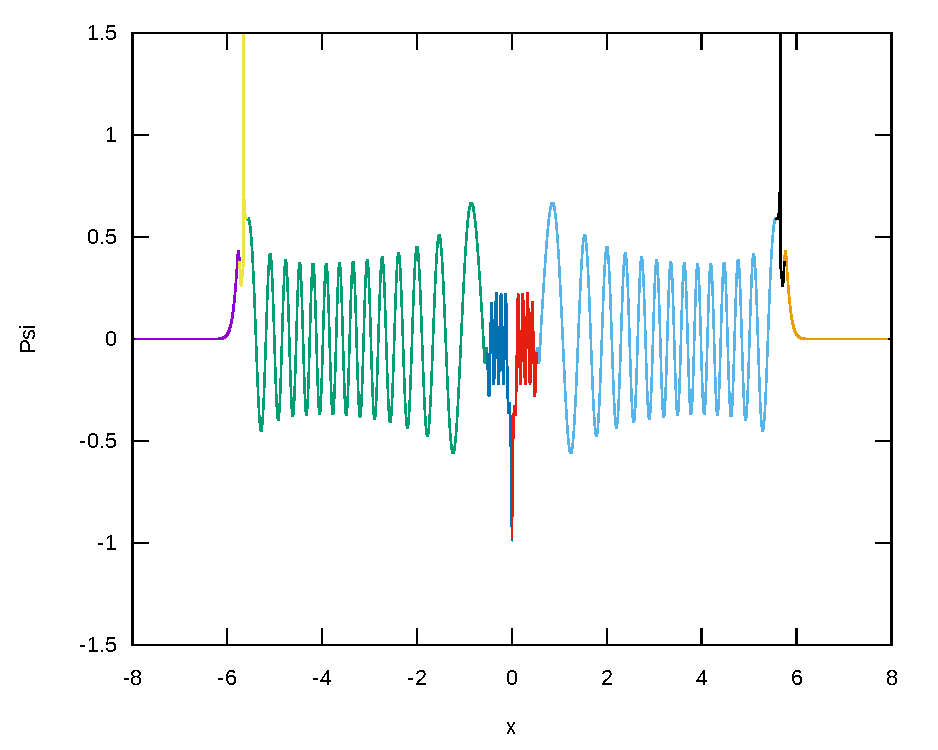
\includegraphics[width=\textwidth]{plots/mexican-hat-54.pdf}
    \caption{
      Wave function of mexican hat potential, with the 54th energy and $m = 1$. The program could not find all the turning points, that's why there are two asymptotes at the turning points.
      Around $x = 0$ it oscillates with a high frequency even though a small frequency was expected.
    }\label{fig:mexican-hat-54th-energy}
\end{figure}


\section{Proofs}
\subsection{Smoothness of Transition Function}\label{proof:joint}
Given that
\begin{align}
  f: \mathbb{R} \rightarrow \mathbb{C} \\
  g: \mathbb{R} \rightarrow \mathbb{C} \\
  \{f, g\} \in C^{1} \\
  \{\alpha, \delta\} \in \mathbb{C}
\end{align}
define \hspace*{\fill}~\citep{hall2013quantum}
\begin{align}
  \chi(x) = \sin^{2}\left(\cfrac{\pi(x - \alpha)}{2\delta}\right) \\
  (f \sqcup g)(x) = f(x) + (g(x) - f(x)) \chi(x)
\end{align}
and proof that
\begin{align}
  \label{eq:deriv-f}
  \cfrac{d(f \sqcup g)}{dx}(\alpha) = \cfrac{df}{dx}(\alpha) \\
  \label{eq:deriv-g}
  \cfrac{d(f \sqcup g)}{dx}(\alpha + \delta) = \cfrac{dg}{dx}(\alpha + \delta).
\end{align}
Calculate derivatives
\begin{align}
  \deriv{\chi}{x}(x) = \cfrac{\pi}{2 \delta} \sin\left(\cfrac{\pi (x - \alpha)}{\delta}\right)\\
  \deriv{(f \sqcup g)}{x}(x) = \deriv{f}{x}(x) + \left(\deriv{g}{x}(x) - \deriv{f}{x}(x)\right)\chi(x) + (g(x) - f(x))\deriv{\chi}{x}(x).
\end{align}
Note that
\begin{align}
  \deriv{\chi}{x}(\alpha) = 0 \\
  \chi(\alpha) = 0 \\
  \deriv{\chi}{x}(\alpha + \delta) = 0 \\
  \chi(\alpha + \delta) = 1
\end{align}
therefore
\begin{align}
  \deriv{(f \sqcup g)}{x}(\alpha) = \deriv{f}{x}(\alpha) + 0 \left(\deriv{g}{x}(\alpha) - \deriv{f}{x}(\alpha)\right) + 0 (g(x) - f(x)) = \deriv{f}{x}(\alpha)
\end{align}
and
\begin{align}
  \deriv{(f \sqcup g)}{x}(\alpha + \delta) = \deriv{f}{x}(\alpha + \delta) + 1 \left(\deriv{g}{x}(\alpha + \delta) - \deriv{f}{x}(\alpha + \delta)\right) + 0 (g(x) - f(x)) \\
  \deriv{(f \sqcup g)}{x}(\alpha + \delta) = \deriv{f}{x}(\alpha + \delta) + \deriv{g}{x}(\alpha + \delta) - \deriv{f}{x}(\alpha + \delta) = \deriv{g}{x}(\alpha + \delta)~\blacksquare.
\end{align}

\section{Validity of 0 Wave Function}\label{proof:zero-wave-function}
\begin{align}
  \Psi(x) = 0 \\
  \frac{1}{2m} \frac{d^{2}}{dx^{2}}\Psi(x) + V(x) \Psi(x)  = E \Psi(x) \\
  \frac{1}{2m} \cdot 0 + V(x) \cdot 0 = E \cdot 0 \\
  0 = 0~\blacksquare
\end{align}
There for $\Psi(x) = 0$ is a solution for all energies and all potentials.
\section{Branch Elimination}\label{test:branch-elim}
To check if branches with a constant condition of \rustinline{false} gets removed we will use ``Compiler Explorer'' on \url{https://godbolt.org/}.
This is an online tool to generate the assembly of source code.
The settings used for this test are ``Rust'' for the language, ``rustc 1.65.0'' for the compiler with flags ``-O''.
\\[1ex]
\begin{paracol}{2}
{\noindent \bfseries Rust Code}
\begin{rustcode}[numbers=none]
const COND: bool = true;

pub fn test(x: f64) -> f64 {
    if x > 5.0 && COND {
        return x % 5.0;
    } else {
        return x*x;
    }
}
\end{rustcode}
\switchcolumn
{\noindent \bfseries Assembly}
\begin{bashcode}[numbers=none]
.LCPI0_0:
        .quad   0x4014000000000000
example::test:
        push    rax
        ucomisd xmm0, qword ptr [rip + .LCPI0_0]
        jbe     .LBB0_1
        movsd   xmm1, qword ptr [rip + .LCPI0_0]
        call    qword ptr [rip + fmod@GOTPCREL]
        pop     rax
        ret
.LBB0_1:
        mulsd   xmm0, xmm0
        pop     rax
        ret
\end{bashcode}
\end{paracol}
As we can see in the \rustinline{true} case the \bashinline{.LBB0_1} label was inserted which means the code will branch.
\\[1ex]
\begin{paracol}{2}
{\noindent \bfseries Rust Code}
\begin{rustcode}[numbers=none]
const COND: bool = false;

pub fn test(x: f64) -> f64 {
    if x > 5.0 && COND {
        return x % 5.0;
    } else {
        return x*x;
    }
}
\end{rustcode}
\switchcolumn
{\noindent \bfseries Assembly}
\begin{bashcode}[numbers=none]
example::test:
        mulsd   xmm0, xmm0
        ret
\end{bashcode}
\end{paracol}
In the \rustinline{false} case the compiler directly calculates $x^{2}$ directly without any checks since the first condition is always \rustinline{false}.

\chapter{Data Files}
\section{Energies}

\begin{paracol}{2}
\bashinline{energies_approx.dat}\label{dat:energy-rs}
\begin{lstlisting}[numbers=none]
0 0.7071985499773434
1 2.121283145049141
2 3.535523992562384
3 4.949764840075626
4 6.364005687588868
5 7.778246535102111
6 9.192487382615353
7 10.606571982569964
8 12.020812830083207
9 13.435366182479338
10 14.849294525109691
11 16.263535372622933
12 17.67761996769473
13 19.091860815207973
14 20.506257920045474
15 21.92034251511727
16 23.33442711018907
17 24.74866795770231
18 26.163221310098443
19 27.577305905170242
20 28.99185925756637
21 30.40578760507954
22 31.82002845259278
23 33.23442555254747
24 34.648041390294935
25 36.062282237808176
26 37.477148095087195
27 38.89076393283466
28 40.305004785230715
29 41.71971439006829
30 43.133330227815755
31 44.547571075328996
32 45.96181192284224
33 47.37636527523837
34 48.79044987031017
35 50.204534470264775
36 51.61908782266091
37 53.03301616529126
38 54.4472570128045
39 55.8613416078763
40 57.27558245538954
41 58.68966705046134
42 60.10453291262317
43 61.518148750370635
44 62.93270210276677
45 64.3472554551629
46 65.76149630267614
47 67.17542464530649
48 68.58935298793685
49 70.00343758789145
50 71.41783468784614
\end{lstlisting}
\switchcolumn{}
\bashinline{energies_exact.dat}\label{dat:energy-wsl}
\begin{lstlisting}[numbers=none]
0 0.7071067811865475
1 2.1213203435596424
2 3.5355339059327373
3 4.949747468305832
4 6.363961030678928
5 7.778174593052022
6 9.192388155425117
7 10.606601717798211
8 12.020815280171307
9 13.435028842544401
10 14.849242404917497
11 16.263455967290593
12 17.677669529663685
13 19.09188309203678
14 20.506096654409877
15 21.920310216782973
16 23.334523779156065
17 24.74873734152916
18 26.162950903902257
19 27.577164466275352
20 28.991378028648445
21 30.40559159102154
22 31.819805153394636
23 33.23401871576773
24 34.648232278140824
25 36.062445840513924
26 37.476659402887016
27 38.89087296526011
28 40.30508652763321
29 41.7193000900063
30 43.13351365237939
31 44.54772721475249
32 45.961940777125584
33 47.37615433949868
34 48.790367901871775
35 50.20458146424487
36 51.61879502661797
37 53.03300858899106
38 54.44722215136415
39 55.86143571373725
40 57.27564927611034
41 58.68986283848344
42 60.104076400856535
43 61.51828996322963
44 62.932503525602726
45 64.34671708797582
46 65.76093065034891
47 67.175144212722
48 68.58935777509511
49 70.0035713374682
50 71.4177848998413
\end{lstlisting}
\end{paracol}

\chapter{Source Code}
\begin{figure}[H]\label{fig:uml-arch}
  \centering
  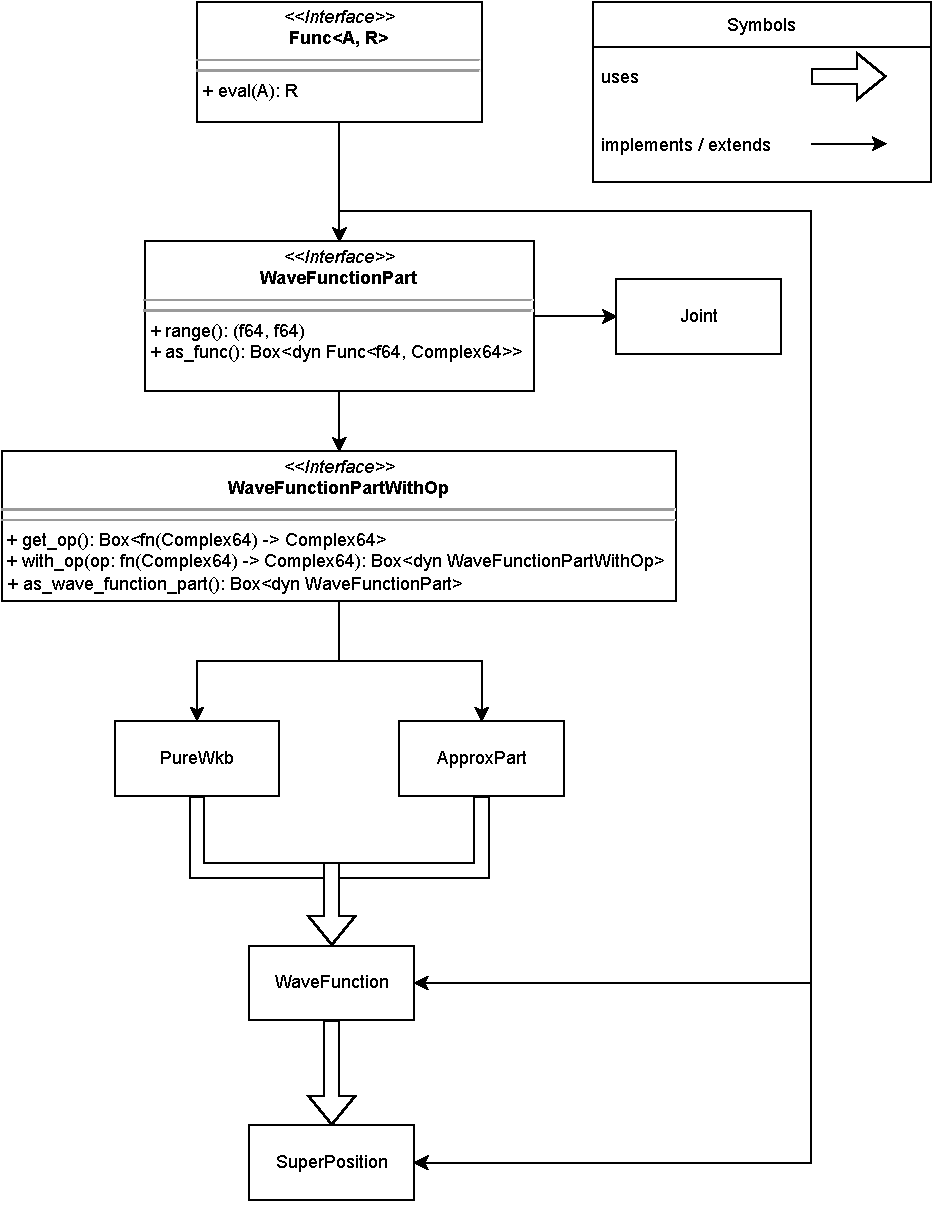
\includegraphics[width=\textwidth]{program_architecture.pdf}
  \caption{UML diagram of program architecture}
\end{figure}

The source code is also available on the authors GitHub \\
\url{https://github.com/Gian-Laager/Schroedinger-Approximation}\\[3ex]
\vspace*{3ex}
{\noindent \large \bfseries build.rs}
\lstinputlisting[language=Rust]{code/build.rs}

\vspace*{3ex}
{\noindent \large \bfseries Cargo.toml}
\lstinputlisting[]{code/Cargo.toml}

\vspace*{3ex}
{\noindent \large \bfseries energy.wsl}
\lstinputlisting[]{code/energy.wsl}

\vspace*{3ex}
{\noindent \large \bfseries exact.wsl}
\lstinputlisting[]{code/exact.wsl}

\vspace*{3ex}
{\noindent \large \bfseries LICENSE}
\lstinputlisting[]{code/LICENSE}

\vspace*{3ex}
{\noindent \large \bfseries README.md}
\lstinputlisting[]{code/README.md}

\vspace*{3ex}
{\noindent \large \bfseries lib/build.sh}
\lstinputlisting[language=bash]{code/lib/build.sh}

\vspace*{3ex}
{\noindent \large \bfseries lib/go.mod}
\lstinputlisting[]{code/lib/go.mod}

\vspace*{3ex}
{\noindent \large \bfseries lib/go.sum}
\lstinputlisting[]{code/lib/go.sum}

\vspace*{3ex}
{\noindent \large \bfseries lib/libairy.h}
\lstinputlisting[language=C]{code/lib/libairy.h}

\vspace*{3ex}
{\noindent \large \bfseries lib/main.go}
\lstinputlisting[language=Go]{code/lib/main.go}

\vspace*{3ex}
{\noindent \large \bfseries src/airy.rs}
\lstinputlisting[language=Rust]{code/src/airy.rs}

\vspace*{3ex}
{\noindent \large \bfseries src/airy\_wave\_func.rs}
\lstinputlisting[language=Rust]{code/src/airy_wave_func.rs}

\vspace*{3ex}
{\noindent \large \bfseries src/benchmarks.rs}
\lstinputlisting[language=Rust]{code/src/benchmarks.rs}

\vspace*{3ex}
{\noindent \large \bfseries src/check.rs}
\lstinputlisting[language=Rust]{code/src/check.rs}

\vspace*{3ex}
{\noindent \large \bfseries src/energy.rs}
\lstinputlisting[language=Rust]{code/src/energy.rs}

\vspace*{3ex}
{\noindent \large \bfseries src/integrals.rs}
\lstinputlisting[language=Rust]{code/src/integrals.rs}

\vspace*{3ex}
{\noindent \large \bfseries src/main.rs}
\lstinputlisting[language=Rust]{code/src/main.rs}

\vspace*{3ex}
{\noindent \large \bfseries src/newtons\_method.rs}
\lstinputlisting[language=Rust]{code/src/newtons_method.rs}

\vspace*{3ex}
{\noindent \large \bfseries src/plot.rs}
\lstinputlisting[language=Rust]{code/src/plot.rs}

\vspace*{3ex}
{\noindent \large \bfseries src/potentials.rs}
\lstinputlisting[language=Rust]{code/src/potentials.rs}

\vspace*{3ex}
{\noindent \large \bfseries src/tui.rs}
\lstinputlisting[language=Rust]{code/src/tui.rs}

\vspace*{3ex}
{\noindent \large \bfseries src/turning\_points.rs}
\lstinputlisting[language=Rust]{code/src/turning_points.rs}

\vspace*{3ex}
{\noindent \large \bfseries src/utils.rs}
\lstinputlisting[language=Rust]{code/src/utils.rs}

\vspace*{3ex}
{\noindent \large \bfseries src/wave\_function\_builder.rs}
\lstinputlisting[language=Rust]{code/src/wave_function_builder.rs}

\vspace*{3ex}
{\noindent \large \bfseries src/wkb\_wave\_func.rs}
\lstinputlisting[language=Rust]{code/src/wkb_wave_func.rs}

\end{appendix}
\bibliographystyle{plainnatromer}
\bibliography{marbeit}

%
\chapter*{Selbständigkeitserklärung}
%
Hiermit bestätige ich, Gian Laager, meine Maturaarbeit selbständig verfasst und alle Quellen angegeben zu haben.\\\newline
Ich nehme zur Kenntnis, dass meine Arbeit zur Überprüfung der korrekten und vollständigen Angabe der Quellen mit Hilfe einer Software (Plagiaterkennungstool) geprüft wird. Zu meinem eigenen Schutz wird die Software auch dazu verwendet, später eingereichte Arbeiten mit meiner Arbeit elektronisch zu vergleichen und damit Abschriften und eine Verletzung meines Urheberrechts zu verhindern. Falls Verdacht besteht, dass mein Urheberrecht verletzt wurde, erkläre ich mich damit einverstanden, dass die Schulleitung meine Arbeit zu Prüfzwecken herausgibt.\\\newline
Ort\hspace{4cm} Datum\hspace{4cm}  Unterschrift
%
\end{document}
